\documentclass[english,10pt,a4paper,titlepage]{report}
\usepackage{babel}
\usepackage[utf8]{inputenc}
\usepackage{graphicx}
%\usepackage{lscape}
\usepackage{natbib}
\usepackage{amsmath}
\usepackage{multirow}
\usepackage{hyperref}
\usepackage{caption}
\usepackage{subcaption}
%\usepackage{geometry}
\usepackage{xcolor}
\usepackage{adjustbox}
\usepackage{array}
\usepackage{booktabs}
\usepackage{tabularx}
\usepackage{booktabs}
\usepackage{pdflscape}
\usepackage{longtable}
\usepackage[left=1in, right=1in, top=1in, bottom=1in]{geometry}
%\hypersetup{colorlinks=true,citecolor=cyan,urlcolor=cyan,linkcolor=blue}
%\newcolumntype{C}{>{\centering\arraybackslash}X}

\setkeys{Gin}{draft=False} %if True, all figures will print as just an empty box (useful when you don't want to wait for an entire dissertation with figures to compile)

% Define URLs
\urldef{\helioweatherurl}\url{http://helioweather.net/archive/}

% define sympol
\newcommand{\degree}{$\,^o\,$}
\newcommand{\almost}{$\,\sim\,$}
\newcommand{\rsun}{$\,R_\odot\,$}
\newcommand{\percc}{$\,cm^{-3}\,$}
\newcommand{\kms}{$\,km\,s^{-1}\,$}

% Journals appreviations
\newcommand{\apj}{Astrophys. J.}
\newcommand{\aap}{Astron. Astrophys.}
\newcommand{\apjl}{Astrophys. J. Lett.}
\newcommand{\apjs}{Astrophys. J. Suppl.}
\newcommand{\solphys}{Sol. Phys.}
\newcommand{\mnras}{Mon. Not. R. Astron. Soc.}

\newcommand{\mnedal}[1]{\textbf{\textcolor{blue}{(Mohamed: #1)}}}


% Use the sectsty package to modify section titles
\usepackage{sectsty}

% Set the font size for the body text
\renewcommand{\normalsize}{\fontsize{12}{15}\selectfont}

% Exclude the title page and section titles from font size change
\sectionfont{\fontsize{12}{15}\selectfont}
\subsectionfont{\fontsize{12}{15}\selectfont}
\subsubsectionfont{\fontsize{12}{15}\selectfont}



\begin{document}
	
	\begin{titlepage}
    \begin{center}
        \vspace*{1cm}
        
        \Huge
        \textbf{From the Sun to Earth: Exploring the Multifaceds of Solar Eruptive Events}
        
        \vspace{1.5cm}
        
        \LARGE
        Mohamed Nedal
        
        \vfill
        
        A thesis submitted for the degree of\\
        Doctor of Philosophy
        
        \vspace{0.8cm}
        
        \Large
        Institute of Astronomy and National Astronomical Observatory, Bulgarian Academy of Sciences\\
        Solar and Space Weather Research\\
        \today
        
        \vspace{0.8cm}
        
        Supervisor: Assoc. Prof. Kamen Asenov Kozarev
        
    \end{center}
\end{titlepage}

	\pagenumbering{roman}
	
	\chapter*{Acknowledgments}
	To my family, professors, and friends ...
	
	\chapter*{}
	This interdisciplinary thesis advances our understanding of solar transients by investigating the early dynamics of Coronal Bright Fronts (CBFs), diagnosing solar Type III radio bursts, and forecasting Solar Energetic Proton (SEP) integral fluxes. Integrating these studies, we reveal the relationships among these phenomena and their implications for space weather forecasting and hazard mitigation. Our analysis of 26 CBFs, using the SPREAdFAST framework and data from AIA and LASCO instruments, unveils temporal evolution, plasma properties, and compressional characteristics. The second study, employing LOFAR and PSP, characterizes 9 Type III radio bursts in the combined dynamic spectrum and 16 in the LOFAR spectrum alone. PFSS and MHD models offer insights into plasma conditions and magnetic fields, advancing our understanding of Type III radio bursts triggered by accelerated electrons associated with CBFs and solar flares. Addressing forecasting, a BiLSTM neural network using OMNIWeb data from 1976 to 2019 predicts SEP fluxes, emphasizing the hazardous influence of energetic particles on Earth and technology. This work provides a unified framework, highlighting the interconnected nature of solar transients and their collective impact on space weather.

	
	\tableofcontents
	\listoftables
	\listoffigures
	
	\newpage
	\chapter*{Definitions and Acronyms}
	Here, I provide definitions for key domain-specific terms and measurement concepts used consistently throughout the thesis. Additionally, relevant terminology will be introduced within the corresponding chapters. Below is a compilation of the essential technical terms and acronyms featured in this work:

\vspace{0.5cm}

CME -- Coronal Mass Ejection

ICME -- Interplanetary Coronal Mass Ejection

SF -- Solar Flare

CIR -- Corotating Interaction Region

IMF -- Interplanetary Magnetic Field

GS -- Geomagnetic Storm

Dst -- Disturbance storm time

AU -- Astronomical Unit

MPA -- Measurement Position Angle

SEPs -- Solar Energetic Particles/Protons

ESP -- Energetic Storm Particle

EUV -- Extreme Ultra-Violet

CBF -- Coronal Bright Front

SRB -- Solar Radio Burst

DH -- Decameter-Hectometric

SOHO -- Solar and Heliospheric Observatory

LASCO -- Large Angle and Spectrometric Coronagraph

ERNE -- Energetic and Relativistic Nuclei and Electron

EIT -- Extreme ultraviolet Imaging Telescope

TRACE -- Transition Region and Coronal Explorer

ESA -- European Space Agency

MHD -- Magneto-Hydro-Dynamic

MAS -- Magnetohydrodynamic Algorithm outside a Sphere

PSI -- Predictive Science Inc.

PFSS -- Potential Field Source Surface

AIA -- Atmospheric Imaging Assembly

SDO -- Solar Dynamic Observatory

EUVI -- Extreme Ultraviolet Imager

STEREO -- Solar Terrestrial Relations Observatory

LOFAR -- Low-Frequency Array

PSP -- Parker Solar Probe

GOES -- Geostationary Operational Environmental Satellite

SN -- Sunspot Number

SC -- Solar Cycle

sfu -- solar flux units

pfu -- proton flux units

L1 -- First Lagrange point

SPDF -- Space Physics Data Facility

SILSO -- Sunspot Index and Long-term Solar Observations

NOAA -- National Oceanic and Atmospheric Administration

NASA -- National Aeronautics and Space Administration

GSFC -- Goddard Space Flight Center

SPREAdFAST -- Solar Particle Radiation Environment Analysis and Forecasting–Acceleration and Scattering Transport

CASHeW -- Coronal Analysis of SHocks and Waves

DSA -- Diffusive Shock Acceleration

SDA -- Shock Drift Acceleration

S2M -- Synthetic Shock Model

EPREM -- Energetic Particle Radiation Environment Module

DEM -- Differential Emission Measure

FLCT -- Fourier Local Correlation Tracking

CM -- Centers of Mass

GC -- Geometric Center

GCS -- Graduated Cylindrical Shell

NN -- Neural Network

ML -- Machine Learning

DL -- Deep Learning

CNN -- Convolutional Neural Network

GAN -- Generative Adversarial Networks

RNN -- Recurrent Neural Network

BiLSTM -- Bi-directional Long short-term Memory

Adam -- Adaptive moment estimation

MIMO -- Multi-Input Multiple Output

MSE -- Mean Squared Error

MAE -- Mean Absolute Error

MSLE -- Mean Squared Logarithmic Error

TP -- True Positive

TN -- True Negative

FP -- False Positive

FN -- False Negative

POD -- Probability of Detection

POFD -- Probability of False Detection

FAR -- False Alarm Rate

CSI -- Critical Success Index

TSS -- True Skill Statistic

HSS -- Heidke Skill Score
	
	\pagenumbering{arabic}
	
	\chapter{Introduction}
\label{chapter1}

\section{Background and Motivation}
The Sun, an ordinary main-sequence star situated at the center of our Solar System, exhibits various forms of activity and variability on multiple spatial and temporal scales (Priest, 2014; Aschwanden, 2006). One of the main manifestations of solar activity relevant to space weather research are transient energetic eruptive phenomena such as flares, coronal mass ejections (CMEs), and wide-ranging emissions of electromagnetic radiation and energetic particles (Schwenn, 2006; Pulkkinen, 2007). These eruptive events originate due to the sudden release of free magnetic energy stored in complex, twisted or sheared magnetic field structures in the solar atmosphere (Forbes et al., 2006; Chen, 2011; Priest and Forbes, 2007). The energetic phenomena are driven by the rapid dissipation of magnetic energy via magnetic reconnection which can accelerate large numbers of electrons to relativistic energies and heat plasma to tens of million Kelvin (Shibata and Magara, 2011; Benz, 2017).

The eruptive solar events drive major disturbances in the near-Earth space environment and planetary environments across the heliosphere, collectively termed space weather (Schrijver and Siscoe, 2010; Eastwood et al., 2017). Enhanced fluxes of solar energetic particles (SEPs), plasma ejecta, and electromagnetic radiation emitted during solar eruptions can impact the geomagnetic field, radiation belts, ionosphere, thermosphere, and upper atmosphere surrounding the Earth (Schwenn, 2006; Pulkkinen, 2007). Adverse effects range from disruption of radio communications to damage of satellites, power grid failures, aviation hazards due to radiation risks for airline crew and passengers, and increased radiation exposure for astronauts (ISO, 2015; Lanzerotti, 2001). The societal dependence on space-based infrastructure has increased exponentially, escalating the vulnerability to space weather disturbances. Recent studies estimate a severe space weather event could lead to trillion-dollar economic damages in the US alone (Oughton et al., 2017). Besides the near-Earth space environment, solar eruptive transients also drive adverse space weather effects across the Solar System impacting activities such as deep space exploration and astronomy (Luhmann et al., 2010; Lilensten et al., 2014).

Therefore, advancing our understanding of the origins and propagation characteristics of solar eruptive phenomena, as well as quantifying their impacts on geospace and planetary environments, has become an extremely important pursuit for nations worldwide. Fundamental research seeks to uncover the physical processes involved using observations coupled with theory and modeling (Schrijver et al., 2015). Concurrently, significant efforts are underway to develop next-generation space environment modeling and forecasting capabilities for predicting the impacts of solar variability (Spann et al., 2014). The field combining these research and predictive aspects related to Sun-Earth connections is broadly termed heliophysics (Schrijver and Siscoe, 2010). It encompasses understanding the fundamental solar, heliospheric and geospace plasma processes; coupling across multiple spatial and temporal scales; quantifying the impacts on humanity's technological systems and space-borne assets; and utilizing this knowledge to prevent/mitigate adverse effects (Schrijver et al., 2015). NASA's Living With a Star program and the Naional Science Foundation's Space Weather activities exemplify strategic efforts to advance scientific understanding and predictive capabilities across the interconnected domains of heliophysics (Koskinen et al., 2017; NSF, 2018).

The present thesis focuses on studying several important phenomena related to solar eruptive activity and its impacts from the perspective of heliophysics research and space weather. The specific topics investigated include: (1) The propagation and evolution characteristics of large-scale coronal disturbances termed EUV waves that are triggered by solar flares and CMEs. (2) The generation, propagation and plasma characteristics of solar radio bursts emitted by accelerated electron beams traveling along open magnetic field lines in the corona. (3) The forecasting of gradual solar energetic particle (SEP) events which constitute one of the major components of space radiation hazards at Earth.

These diverse topics are united by the common theme of seeking to uncover the origins and propagation mechanisms of key transient phenomena resulting from solar eruptions, utilizing observational data, analytical theory and modeling, and data science techniques. The phenomena have been studied for several decades using observations from multiple space missions, but gaps persist in our understanding of their underlying physics and space weather impacts. The thesis aims to provide new insights that help address some of the outstanding questions, guided by the overarching goals and framework of heliophysics research. The following sub-sections elaborate on the background, significance, observational challenges and knowledge gaps pertaining to each of the research topics investigated.

\textbf{Coronal Waves}
Coronal waves are large-scale arc-shaped bright fronts observed propagating across significant portions of the solar corona following the eruption of CMEs and flares (Warmuth, 2015). They are best observed in Extreme Ultraviolet (EUV) and white light coronal emission, spanning distances of up to several 100 Mm with speeds ranging from 100-1000 km/s (Liu and Ofman, 2014; Nitta et al., 2013). The discovery of coronal waves dates back to observations obtained with the EIT instrument on SOHO launched in 1995, appearing as bright propagating fronts in 19.5 nm wavelength imaging of Fe XII emission lines formed at ~1.5 MK plasma (Thompson et al., 1998). Since 2010, the initiation and evolution of coronal waves are being exquisitely observed with unprecedented resolution by the SDO/AIA instrument (Lemen et al., 2012) across multiple EUV passbands sensitive to a wide temperature range (Nitta et al., 2013). Coronal waves exhibit diverse morphology and kinematics ranging from circular fronts to narrow jets or expanding dome-like structures (Veronig et al., 2010). A taxonomy of wave properties based on extensive observational surveys can be found in papers by Muhr et al. (2014) and Nitta et al. (2013).

However, despite being observed for over two decades since their serendipitous discovery, fundamental questions remain regarding the physical nature and drivers of coronal waves (Chen, 2016; Vršnak and Cliver, 2008; Warmuth, 2015). The debate centers around two competing interpretations - the wave versus pseudo-wave (or non-wave) models. The wave models envisage coronal waves as fast-mode MHD waves or shocks that propagate freely after being launched by a CME lateral over-expansion or an initial flare pressure pulse (Wills-Davey et al., 2007; Vršnak and Cliver, 2008). The pseudo-wave models interpret them as bright fronts produced by magnetic field restructuring related to the CME lift-off process rather than a true wave disturbance (Delannée and Aulanier, 1999; Chen et al., 2002). Extensive observational and modeling studies have been undertaken to evaluate the two paradigms (Patsourakos and Vourlidas, 2012; Long et al., 2017), but a consensus remains elusive. Addressing these outstanding questions related to the nature and origin of coronal waves is imperative, since they are being incorporated into models as a primary agent producing SEP events and geomagnetic storms during CMEs (Rouillard et al. 2012; Park et al. 2013). Their use as a diagnostic tool for CME and shock kinematics predictions in these models requires discriminating between the different physical mechanisms proposed for their origin.

The present thesis undertakes an extensive statistical analysis of coronal EUV wave events observed by SDO to provide new insights into their kinematical properties and relationship to CMEs. We focus on analyzing their large-scale evolution as a function of distance and direction from the source region, leveraging the extensive EUV full-disk imaging capabilities of SDO spanning nearly a decade. Statistical surveys to date have mostly focused on initial speeds and morphological classifications rather than large-scale propagation characteristics. Our study aims to uncover systematic trends in their propagation kinematics using a significantly larger sample compared to previous works. We also comprehensively evaluate associations with CME and flare parameters in order to discriminate between wave and pseudo-wave origins. The results have important implications for incorporating coronal waves into predictive models of CMEs and SEP events for future space weather forecasting.

\textbf{Solar Radio Bursts}
Solar radio bursts provide remote diagnostics of energetic electrons accelerated in the corona and their transport along magnetic field lines (Reid and Ratcliffe, 2014). They are produced by non-thermal electron distributions interacting with the ambient plasma to generate electromagnetic emission at radio frequencies via plasma emission mechanisms (Melrose, 1980). The bursts appear as intense enhancements of radio flux over background levels across a broad range of frequencies from kHz to GHz, often exhibiting rapid drifts from high to low frequencies over seconds to minutes signifying plasma dynamics (Reid and Vilmer, 2017). Radio imaging spectroscopy using interferometric imaging arrays coupled with high time/frequency resolution spectrometers enables tracking radio sources as a function of frequency and position on the Sun, yielding particle acceleration locations and trajectories through the corona into interplanetary space (Krucker et al., 1999; Klassen et al., 2003). This provides a unique diagnostic of energetic particle transport from the Sun to the Earth which is crucial for improving SEP forecasting models.

Different types of bursts are observed, classified based on their spectral characteristics as documented in radio burst catalogs (Sales et al., 2019; Smirnova et al., 2013). The present thesis focuses on detailed analysis of solar type III radio bursts and their associated phenomena (Reid and Ratcliffe, 2014). Type III bursts appear as intense rapidly drifting emissions from high to low frequencies over seconds, corresponding to the propagation of energetic electron beams from the low corona to beyond 1 AU along open field lines. They signify the initial escape of flare-accelerated electrons into interplanetary space, making them an important precursor signature of SEP activity (Cane et al., 2002; MacDowall et al., 2003). Investigating their source locations, plasma environments, and beam kinematics based on multiwavelength observations coupled with plasma emission theory is therefore vital for improved understanding of coronal particle acceleration and transport processes relevant for SEP forecasting models.

While type III bursts have been studied for over 50 years since their initial discovery by Wild (1950), gaps persist in our understanding of their exciter beams and emission mechanisms. Key outstanding questions pertain to the detailed electron acceleration and injection sites, beam configurations and energy spectra, drivers of burst onset and duration, and the role of density fluctuations in propagating beams (Reid and Kontar, 2018; Li et al., 2011). Advancing our knowledge of these aspects through coordinated observations and modeling can help constrain the predictions of energetic electron properties based on radio diagnostics. The present work undertakes detailed investigation of a solar type III burst combining imaging and radio spectral data to derive electron beam trajectories and coronal densities, and models the emission sources. The results provide insights into the corona plasma environment and energetic electron transport relevant for SEP forecasting applications.

\textbf{Solar Energetic Particle (SEP) Forecasting}
The arrival of solar energetic particles (SEPs) in the near-Earth space environment constitutes one of the major components of adverse space weather (Reames, 1999; Vainio et al., 2009). SEPs consist primarily of protons (and some heavy ions), accelerated to very high energies by CME-driven shock waves during large solar eruptive events. The gradual SEP events, so called due to their long durations from several hours to a few days, involve protons accelerated to energies above ~10 MeV which can penetrate Earth’s magnetic field and atmosphere posing radiation hazards to humans and equipment in space and at polar regions (Reames, 2013). The complex physics of CME shock acceleration combined with modeling the transport of SEPs through turbulent interplanetary magnetic fields presents major challenges for first-principles based SEP forecasting models (Aran et al., 2006; Laitinen and Dalla, 2017). As an alternative approach, empirical and data-driven models based on statistical/machine learning techniques applied to historical SEP event data have shown considerable promise for operational forecasting over the past decade (Laurenza et al., 2009; Camporeale, 2019). This motivates detailed investigation of data-driven SEP forecasting models using state-of-the-art machine learning algorithms which can outperform conventional empirical methods.

In the present work, we develop a deep neural network model for predicting the intensity profile of >10 MeV gradual SEP proton events utilizing near real-time solar wind plasma measurements as model inputs. Deep learning techniques can capture complex nonlinear relationships between parameters which has been leveraged for diverse space weather applications recently (Camporeale, 2019; Florios et al., 2018). However, applications to SEP forecasting problems are still limited, presenting an important research gap which this thesis aims to address. The developed model is trained and tested on a database of historical SEP events spanning solar cycles 23 and 24, with the goal of producing SEP flux forecasts over an hour in advance of particle arrivals near Earth. Such capability can provide actionable information for mitigating radiation effects from extreme SEP events. The study demonstrates the potential of state-of-the-art machine learning algorithms to achieve significant enhancement of SEP forecasting capabilities building upon conventional empirical methods.


\section{Objectives and Scope}
The primary objectives and research questions addressed through the investigations carried out in this thesis include:

\begin{enumerate}
    \item Characterize the large-scale propagation kinematics of coronal EUV waves over distances of hundreds of Mm from the eruption source location. Compare observed spatial and temporal variations in speeds with analytical CME-driven wave/shock models.
    \item Conduct a comprehensive statistical analysis correlating properties of EUV waves with associated CME and flare parameters utilizing a large event sample. Discriminate between wave and pseudo-wave models based on observational evidence.
    \item Analyze coordinated observations of a solar type III radio burst across imaging and radio spectral domains to derive coronal density profiles, electron beam kinematics and emission source models.
    \item Develop a deep neural network model for forecasting the intensity profile of >10 MeV gradual SEP proton events using real-time solar wind data as inputs. Evaluate model performance and forecast accuracy over different lead times.
\end{enumerate}

The scope of the thesis encompasses key phenomena related to solar eruptions and their space weather impacts that align with the outstanding questions and challenges highlighted in the background discussion. While expansive in scope, some limitations exist that bound the present work:

\begin{itemize}
    \item The studies rely primarily on remote sensing observations of the Sun and heliosphere, limited by measurement capabilities and resolution.
    \item Analytical modeling utilizes simplified theory and assumptions which cannot account for all complexities.
    \item Machine learning models have dependencies on data coverage and uncertainties in input parameters.
    \item Findings are constrained by the event samples studied and applicability to the broader population.
\end{itemize}

These factors imply appropriate care and diligence in interpretation of results and their generalizability. Nevertheless, the present work establishes an important foundation for future advances that can build upon these limitations.

\textbf{Literature Review}
This section provides a concise overview of key literature related to the research topics investigated in the thesis. A detailed review is presented in each chapter specific to the respective phenomenon.

\textit{Coronal Waves}
Early observations of large-scale coronal disturbances were made in white light coronagraph images revealing expanding bright fronts (Hansen et al., 1974; Tappin, 1991). The atmospheric imaging assembly EIT onboard SOHO led to routine observations of "EIT waves" propagating globally across the Sun in EUV lines (Thompson et al., 1998). Subsequent studies based on SOHO/EIT and TRACE imaging found correlations between waves and CMEs, favoring an interpretation as fast-mode MHD waves driven by CME lateral expansions (Biesecker et al., 2002). The arrival of SDO enabled unprecedented high-cadence EUV observations revealing detailed kinematics and morphologies (Liu and Ofman, 2014; Nitta et al., 2013). Contemporary studies using SDO/AIA support a hybrid wave and pseudo-wave picture with both fast-mode waves and magnetic restructuring occurring together (Chen, 2016). The debate continues regarding their true physical nature and origin (Long et al., 2017).

\textit{Solar Radio Bursts}
Pioneering observations of solar radio bursts were made in the 1940s leading to their classifications (Wild et al., 1963). Subsequent spectrographic studies uncovered emission mechanisms, source regions and particle diagnostics (Suzuki and Dulk, 1985). Magnetic reconnection models of flares provided theoretical explanations for particle acceleration generating radio bursts (Holman et al., 2011). Radio imaging enabled direct tracking of type III beam trajectories through corona (Klassen et al., 1999, 2003). Recent work combines imaging and spectral data with modeling to constrain radio burst exciters in unprecedented detail (Chen et al., 2013, Kontar et al. 2017). Key challenges remain in reconciling emission models with observations and predicting radio diagnostics.

\textit{SEP Forecasting}
Initial SEP forecasting models were based on empirical correlations between proton intensity profiles and CME or flare properties (Kahler et al., 2007). More recent work has focused on developing numerical models of CME shock acceleration and SEP transport (Aran et al., 2006; Laitinen and Dalla, 2017). Owing to complex physics involved, operational forecasting relies on empirical and statistical models (Laurenza et al., 2009). The emergence of data science techniques has enabled application of sophisticated machine learning models to SEP forecasting, yielding improved predictions (Camporeale, 2019; Florios et al., 2018). Opportunities exist for novel forecasting approaches utilizing deep learning algorithms and expanded input parameters.

\textbf{Methodology Overview}
The research presented in this thesis employs a synergistic methodology combining analytical theory, numerical modeling, and data science techniques. Both observational case studies and statistical analysis approaches are utilized for gaining new insights from application of these tools. The data sources, models, and algorithms employed in each of the investigations are concisely summarized below.

Coronal waves: The study utilizes an event database of ~200 coronal EUV waves observed by SDO/AIA since 2010, tracking kinematics to >100 Mm distances. Evolution trends are compared with analytical CME-driven wave propagation models. Statistical associations with CME and flare parameters provide corroboration for physical interpretation.

Solar radio bursts: Multiwavelength observations of a type III burst from radio spectrometers and SDO/AIA are analyzed. Beam trajectories, densities, and emission sources are modeled by combining imaging data, plasma emission theory and coronal density models. 

SEP forecasting: A database of >10 MeV SEP events during solar cycles 23-24 is generated using GOES fluxes. A deep neural network model is developed using solar wind data time-series as inputs. Model training, testing and validation is performed to evaluate forecast accuracy over different lead times.

This triangulation between data analysis, physics-based modeling and data-driven modeling provides confidence in the results obtained. Details of the methodological approaches are elaborated in their respective chapters.

\textbf{Main Contributions}
The primary contributions arising from the research presented in this thesis include:

- New large-scale kinematical characterization of coronal EUV waves propagating to distances over 100 Mm. Derived velocity and acceleration trends challenge steady-wave behavior assumed in models. 

- Statistical analysis correlating EUV wave and CME/flare properties using a significantly larger event sample compared to prior studies. This enables stronger discrimination between competing initiation models.

- Novel methodology combining radio and EUV observations with analytical modeling to reconstruct plasma environments and electron beam trajectories for a solar type III radio burst.

- Deep learning forecasting model for intense SEP events using an expanded input parameter space based on solar wind data. This demonstrates cutting-edge artificial intelligence capabilities for space weather applications.

- Synergistic approach leveraging analytical theory, numerical modeling and data science techniques to gain new insights on long-standing problems in heliophysics research related to solar eruptions and their space weather impacts. 

These contributions provide advances over prior state-of-the-art in the respective areas. They have implications for improving models used in operational space weather monitoring and forecasting systems, besides progressing fundamental physics understanding of solar and heliospheric phenomena. The results validate the merit of cross-disciplinary studies combining traditional analytical techniques with modern statistical and machine learning methods to enable discoveries from application of these synergies.

\textbf{Future Work}
The research presented in this thesis establishes an important foundation and provides a precursor for future advances that can build upon the present work. Some open questions and promising areas for future investigations include:

- Additional coronal wave statistical studies using expanded event samples and new imaging datasets from Solar Orbiter and ground observatories to improve generalizability of findings.

- Incorporating 3D analytical and numerical coronal wave propagation models for more physics-based forecasting approaches. 

- Modeling mechanisms for type III radio burst onset and time profiles using particle-in-cell and MHD models. 

- Ensemble forecasting models for SEP events combining multiple machine learning algorithms trained on multi-mission data.

- Validation of data-driven models for other solar wind driven geospace extremes such as radiation belt enhancements and ionospheric storms.

- Leveraging new solar observatory missions and assimilative models within operational prediction systems for real-time space weather forecasts.

- Exploring applications of deep learning and physics-informed machine learning to additional outstanding problems in heliophysics and astrophysics.

In summary, the present work opens exciting avenues for more cross-disciplinary studies synthesizing heliophysics domain knowledge with cutting-edge data science and artificial intelligence methods. The new generation of solar, heliospheric and geospace missions will yield transformative observations to continue advancing both science understanding and predictive capabilities.


\section{Outline}
This thesis is divided into the following five chapters:

Chapter 1 - Introduction: Provides a background to the research topics, motivation and context of the work, summary of literature, overview of methodology, and the structure of the thesis. 

Chapter 2 – Propagation and Drivers of Coronal EUV Waves: Presents a statistical analysis of the kinematics and physical interpretation of coronal waves using EUV imaging observations and analytical models.

Chapter 3 – Plasma Environment and Energetics of a Solar Type III Radio Burst: Details a multi-wavelength observational case study of a type III burst combining data analysis and modeling to probe the radio emission physics. 

Chapter 4 – Deep Learning Approach for Forecasting Intense SEP Events: Describes the development and evaluation of a neural network model for predicting SEP properties using solar wind data.

Chapter 5 – Conclusions and Future Outlook: Summarizes the key findings, implications, and limitations of the research studies. Discusses future extensions building on the present work.

The core chapters 2 through 4 present the major research investigations carried out. The multi-faceted phenomena are studied by tailoring the methodology to leverage their key observational signatures. Together they provide new insights on different aspects of solar eruptions and space weather. Each chapter is structured to be reasonably self-contained, with relevant background and literature specific to the phenomenon under study. The findings are synergistic and united by the common thread of employing heliophysics principles to address outstanding questions using cutting-edge analytics.

\textbf{Definitions and Acronyms}
Some of the key technical terms and acronyms used in this thesis are listed below:

SEP - Solar Energetic Particle

CME - Coronal Mass Ejection 

EUV - Extreme Ultraviolet

SOHO - Solar and Heliospheric Observatory

SDO - Solar Dynamics Observatory

AIA - Atmospheric Imaging Assembly 

EIT - Extreme ultraviolet Imaging Telescope

TRACE - Transition Region and Coronal Explorer

LASCO - Large Angle and Spectrometric COronagraph

GOES - Geostationary Operational Environmental Satellite

AI - Artificial Intelligence

MHD - Magnetohydrodynamics

AU - Astronomical Unit

This provides definitions of the major domain-specific terms and measurement concepts used. Additional terminology is introduced as required in the respective chapters.

	\chapter{Multi-Viewpoint Solar Radio Observations: Integrating Space-based and Ground-based Data for Coronal Diagnostics}
\label{chapter2}

\section{Introduction}
Type III radio bursts are manifestations of transient energetic electron beams injected into the solar corona, propagating along the interplanetary magnetic field (IMF) lines \citep{ergun98, pick6, reid20}. As these beams traverse the corona, they trigger plasma waves (also known as Langmuir waves) that are then transformed into radio emission at the local plasma frequency or its harmonic components \citep{melrose17}.
In the radio spectrograms, type III bursts are usually observed as intense emissions that drift in frequency over timescales of several seconds to minutes and over a wide range of frequencies, from metric to decametric wavelengths \citep{wild50, lecacheux89, bonnin8}, making them detectable by ground-based instruments on Earth and various spacecraft within the heliosphere. 
The frequency of the radio emission is directly related to the plasma density, making type III bursts a valuable diagnostic tool for examining the inner heliosphere and the processes that drive solar active phenomena, such as solar flares and coronal mass ejections \citep{reid14, kontar17}.

The electron beams follow open magnetic field lines and can persist well beyond 1 astronomical unit (AU) (e.g., \citet{dulk85, boudjada20}), offering in situ insights into the burst and ambient conditions of the heliosphere, including electron density, radio frequency drift, speed of the electron beams and even potential direct detection of Langmuir waves (see \citet{gurnett76, gurnett77} and \citet{reid14} and references within). In addition, tracing the path of type III bursts provides a map of the density structure of the heliosphere, serving as a foundation for developing and testing density models.
Since radio observations below $\sim$10 MHz cannot be accomplished from the ground, it is important to combine high- and low-frequency observations from ground-based and space-borne instruments.
In this work, we perform a study of several type III radio bursts that occurred in close succession on April 3, 2019. We use remote observations of type III radio bursts detected by the Low-Frequency Array \citep[LOFAR]{lofar13} ground-based radio telescope and the Parker Solar Probe \citep[PSP]{fox16} spacecraft during Encounter 2 to study the sources of these radio emissions and to investigate the physical conditions responsible for their generation. Additionally, we incorporate results of two steady-state models of the solar corona: the potential field source surface (PFSS) model \citep{altschuler1969magnetic, schatten1969model} and the magnetohydrodynamic algorithm outside a sphere (MAS) model \citep{mhd99}, to gain a better understanding of the coronal magnetic environment and its role in the acceleration of electrons. 
The ground-based LOFAR imaging observations provide valuable insight into the actual location of the burst sources. This research aims to expand upon current knowledge of the electron beams responsible for triggering type III radio bursts and the coronal conditions they experience. Gaining a deeper insight into this aspect is vital in comprehending other solar phenomena, such as solar energetic particles and solar wind, and how they influence the near-Earth space environment.

A number of recent studies investigate the physical mechanisms responsible for the generation of solar type III radio bursts. 
For example, \citet{chen13} investigated the association of type III bursts with flaring activities in February 2011, via combined multi-wavelength observation from the Solar Dynamic Observatory (SDO) instruments, as well as Wind/WAVE and ground-based instruments. They found that the SDO measurements indicated that type III emission was correlated with a hot plasma (7 MK) at the extreme ultraviolet (EUV) jet's footpoint. 
By using a triangulation method with the Wind and the twin STEREO spacecraft, \citet{bonnin8} reported the first measurements of the beaming characteristics for two type III bursts between 2007-2008, assuming the source was located near the ecliptic plane (see also \citet{reiner9}). They concluded that the individual type III bursts have a broad beaming pattern that is roughly parallel to the Parker spiral magnetic field line at the source.
\citet{saint12} conducted a study on almost 10,000 type III bursts observed by the Nancay Radioheliograph between 1998 and 2008. Their analysis revealed discrepancies in the location of type III sources that may have been caused by a tilted magnetic field. Additionally, they found that the average energy released during type III bursts throughout a solar cycle could be comparable to the energy produced by non-thermal bremsstrahlung mechanisms in nano-flares.
\citet{morosan17} utilized LOFAR data to investigate the statistical characteristics of over 800 type III radio bursts within an eight-hour period on July 9, 2013. They discovered that the drift rates of type III bursts were twice that of type S bursts and plasma emission was the primary emission mechanism for both types.

\citet{pulupa20} introduced a statistical overview of type III radio bursts during the first two PSP solar encounters. While the first encounter in November 2018 revealed a small number of bursts, the second encounter in April 2019 exhibited frequent type III bursts, including continuous occurrences during noise storms. They reported the characteristics of type III bursts with spectral and polarization analysis.

\citet{Krupar_2020} performed a statistical survey of 30 type III radio bursts detected by PSP during the second encounter in April 2019 and estimated their decay times, which were used to estimate the relative electron density fluctuations in the solar wind. They localized radio sources using a polarization-based-radio triangulation technique, which placed the sources near the modeled Parker spiral rooted in the active region AR12738 behind the plane of the sky as seen from Earth.

\citet{Cattell_2021} explored correlations between type III radio bursts and EUV emission in the solar corona. Using coordinated observations from PSP, SDO, and Nuclear Spectroscopic Telescope Array (NuSTAR) on April 12, 2019, they identified periodicities in EUV emission correlated with type III burst rates. The findings suggested impulsive events causing heating and cooling in the corona, possibly nano-flares, despite the absence of observable flares in X-ray and EUV data, which implies periodic non-thermal electron acceleration processes associated with small-scale impulsive events.

\citet{harra2021active} explored the origin of the type III radio bursts we are tackling in this paper and found that electron beams that triggered radio bursts may have emanated from the periphery of an active region that showed significant blue-shifted plasma.
More recently, \citet{badman22} observed a distinct type III radio burst using the PSP and LOFAR between 0.1 and 80 MHz on April 9, 2019, around 12:40 UT, six days after the occurrence of the event analyzed in our study. While no detectable flare activity was linked with the event, a type III noise storm was ongoing during the PSP encounter 2. The authors determined the type III trajectory and reconstructed its source using observations from Wind and STEREO spacecraft, as well as measuring related electron enhancement in situ.

In the last few years, we have witnessed the emergence of modern instruments, such as LOFAR and PSP, that have allowed for the observation of solar radio emissions with higher sensitivity from a better vantage point. Although type III bursts have been extensively studied \citep{dabrowski21}, there are still some unresolved issues regarding the exact mechanism of type III emissions.
For example, it is not yet clear how the electrons are accelerated to the high energies required to generate type III radio bursts or what role the coronal magnetic field plays in this process.
Furthermore, there are inconsistencies between the observations and the models, which need to be resolved in order to gain a more complete understanding of the dynamics of the solar corona. Examples of these inconsistencies are the origin of the type III radio bursts and the discrepancy between the estimated plasma densities from the models and the observations. This paper aims to address these unresolved challenges by using new observations from LOFAR and PSP and models of the solar corona to study the physical mechanisms responsible for the generation of type III bursts.
The data analysis includes a combination of radio spectroscopy and imaging techniques to study the frequency, temporal and spatial variations of the radio bursts. 

The paper is organized as follows. In Section~\ref{s_obs}, we describe the observations of type III radio bursts made with LOFAR and PSP. In Section~\ref{s_methods} we explain the data analysis and modeling techniques used to study these events. In Section~\ref{s_results}, we present the results of our analysis, including an investigation of the potential physical mechanisms responsible for the generation of type III radio bursts and a comparison of the observations with models of the solar corona. Finally, in Section~\ref{s_conclusions}, we summarize our findings and discuss their implications.

\section{Observations}
\label{s_obs}
A number of studies focused on observing the solar radio emissions during the second encounter of the PSP in late 2019 \citep{Krupar_2020, pulupa20, Cattell_2021, harra2021active, badman22}. In this study, our primary emphasis is directed towards investigating a set of type III radio bursts that took place on April 3, 2019, during the time interval spanning from $\sim$12:10 to 12:50 UT. This period coincided with the presence of two distinct active regions (ARs) on the Sun, denoted as AR12737 and AR12738. 
AR12737 was situated on the Sun's near side at coordinates E12$^o$N06$^o$. Notably, this region had eight sunspots and exhibited a $\beta$ magnetic configuration according to the Hale magnetic classification \citep{hale_1919}. On the other hand, AR12738 was positioned on the solar far side at coordinates E140$^o$N02$^o$. Due to its remote location, detailed observations of the magnetic configuration and activity within AR12738 were unattainable in this time frame.

We observed a group of intense type III radio bursts by four instruments (Wind/WAVES, PSP/FIELDS, STEREO-A/SWAVES, and LOFAR/LBA) via a regular survey. In Figure~\ref{fig_alldyspec}, we show the first type III burst within the time of this study as observed by the four instruments. By taking the second derivative of the light curve at a specific frequency channels, we determined the start time of the burst, which is denoted by the vertical red dashed line. The frequency bands used for obtaining the start time at each instrument are as follows: 6.97 MHz (Wind), 7.03 MHz (STEREO), 5.03 MHz (PSP), and 40.16 MHz (LOFAR).

We checked the relative orientations of the instruments with respect to Earth (Fig.~\ref{locations}). Since the PSP and STEREO spacecraft were almost aligned (close in an angular sense) with the Sun, the STEREO/EUVI image could be taken as what PSP would see (Fig.~\ref{soldisk_xrs}).
Figure~\ref{soldisk_xrs} shows how the solar disk looks like from the Earth perspective (using the SDO/AIA instrument) and from the eastern side where the PSP and STEREO were located at that time (using the STEREO/EUVI instrument).
The right panel shows a closer view of AR12737 with the contours of the photospheric magnetic field obtained from the Helioseismic and Magnetic Imager (HMI) on board SDO.
From the GOES-15/XRS and SDO/EVE instruments in the panels below, they also confirm that there is no flaring activity at that time.

The solar disk was quiet, including only one AR that is visible with no X-rays and no EUV transient emissions over this period.
Nevertheless, the very sensitive LOFAR telescope detected a number of bursts close to noon. We checked PSP data, and we found bursts there as well.
Meanwhile, from the EUVI and AIA images, we see that there are numerous small localized regions of relatively higher intensity (i.e., likely small-scale coronal brightenings spots or campfires; see \citet{young18, madjarska19, berghmans21}).
In the next subsections, we introduce the PSP and LOFAR instruments and their observations of the radio bursts.

\begin{figure}
\centering
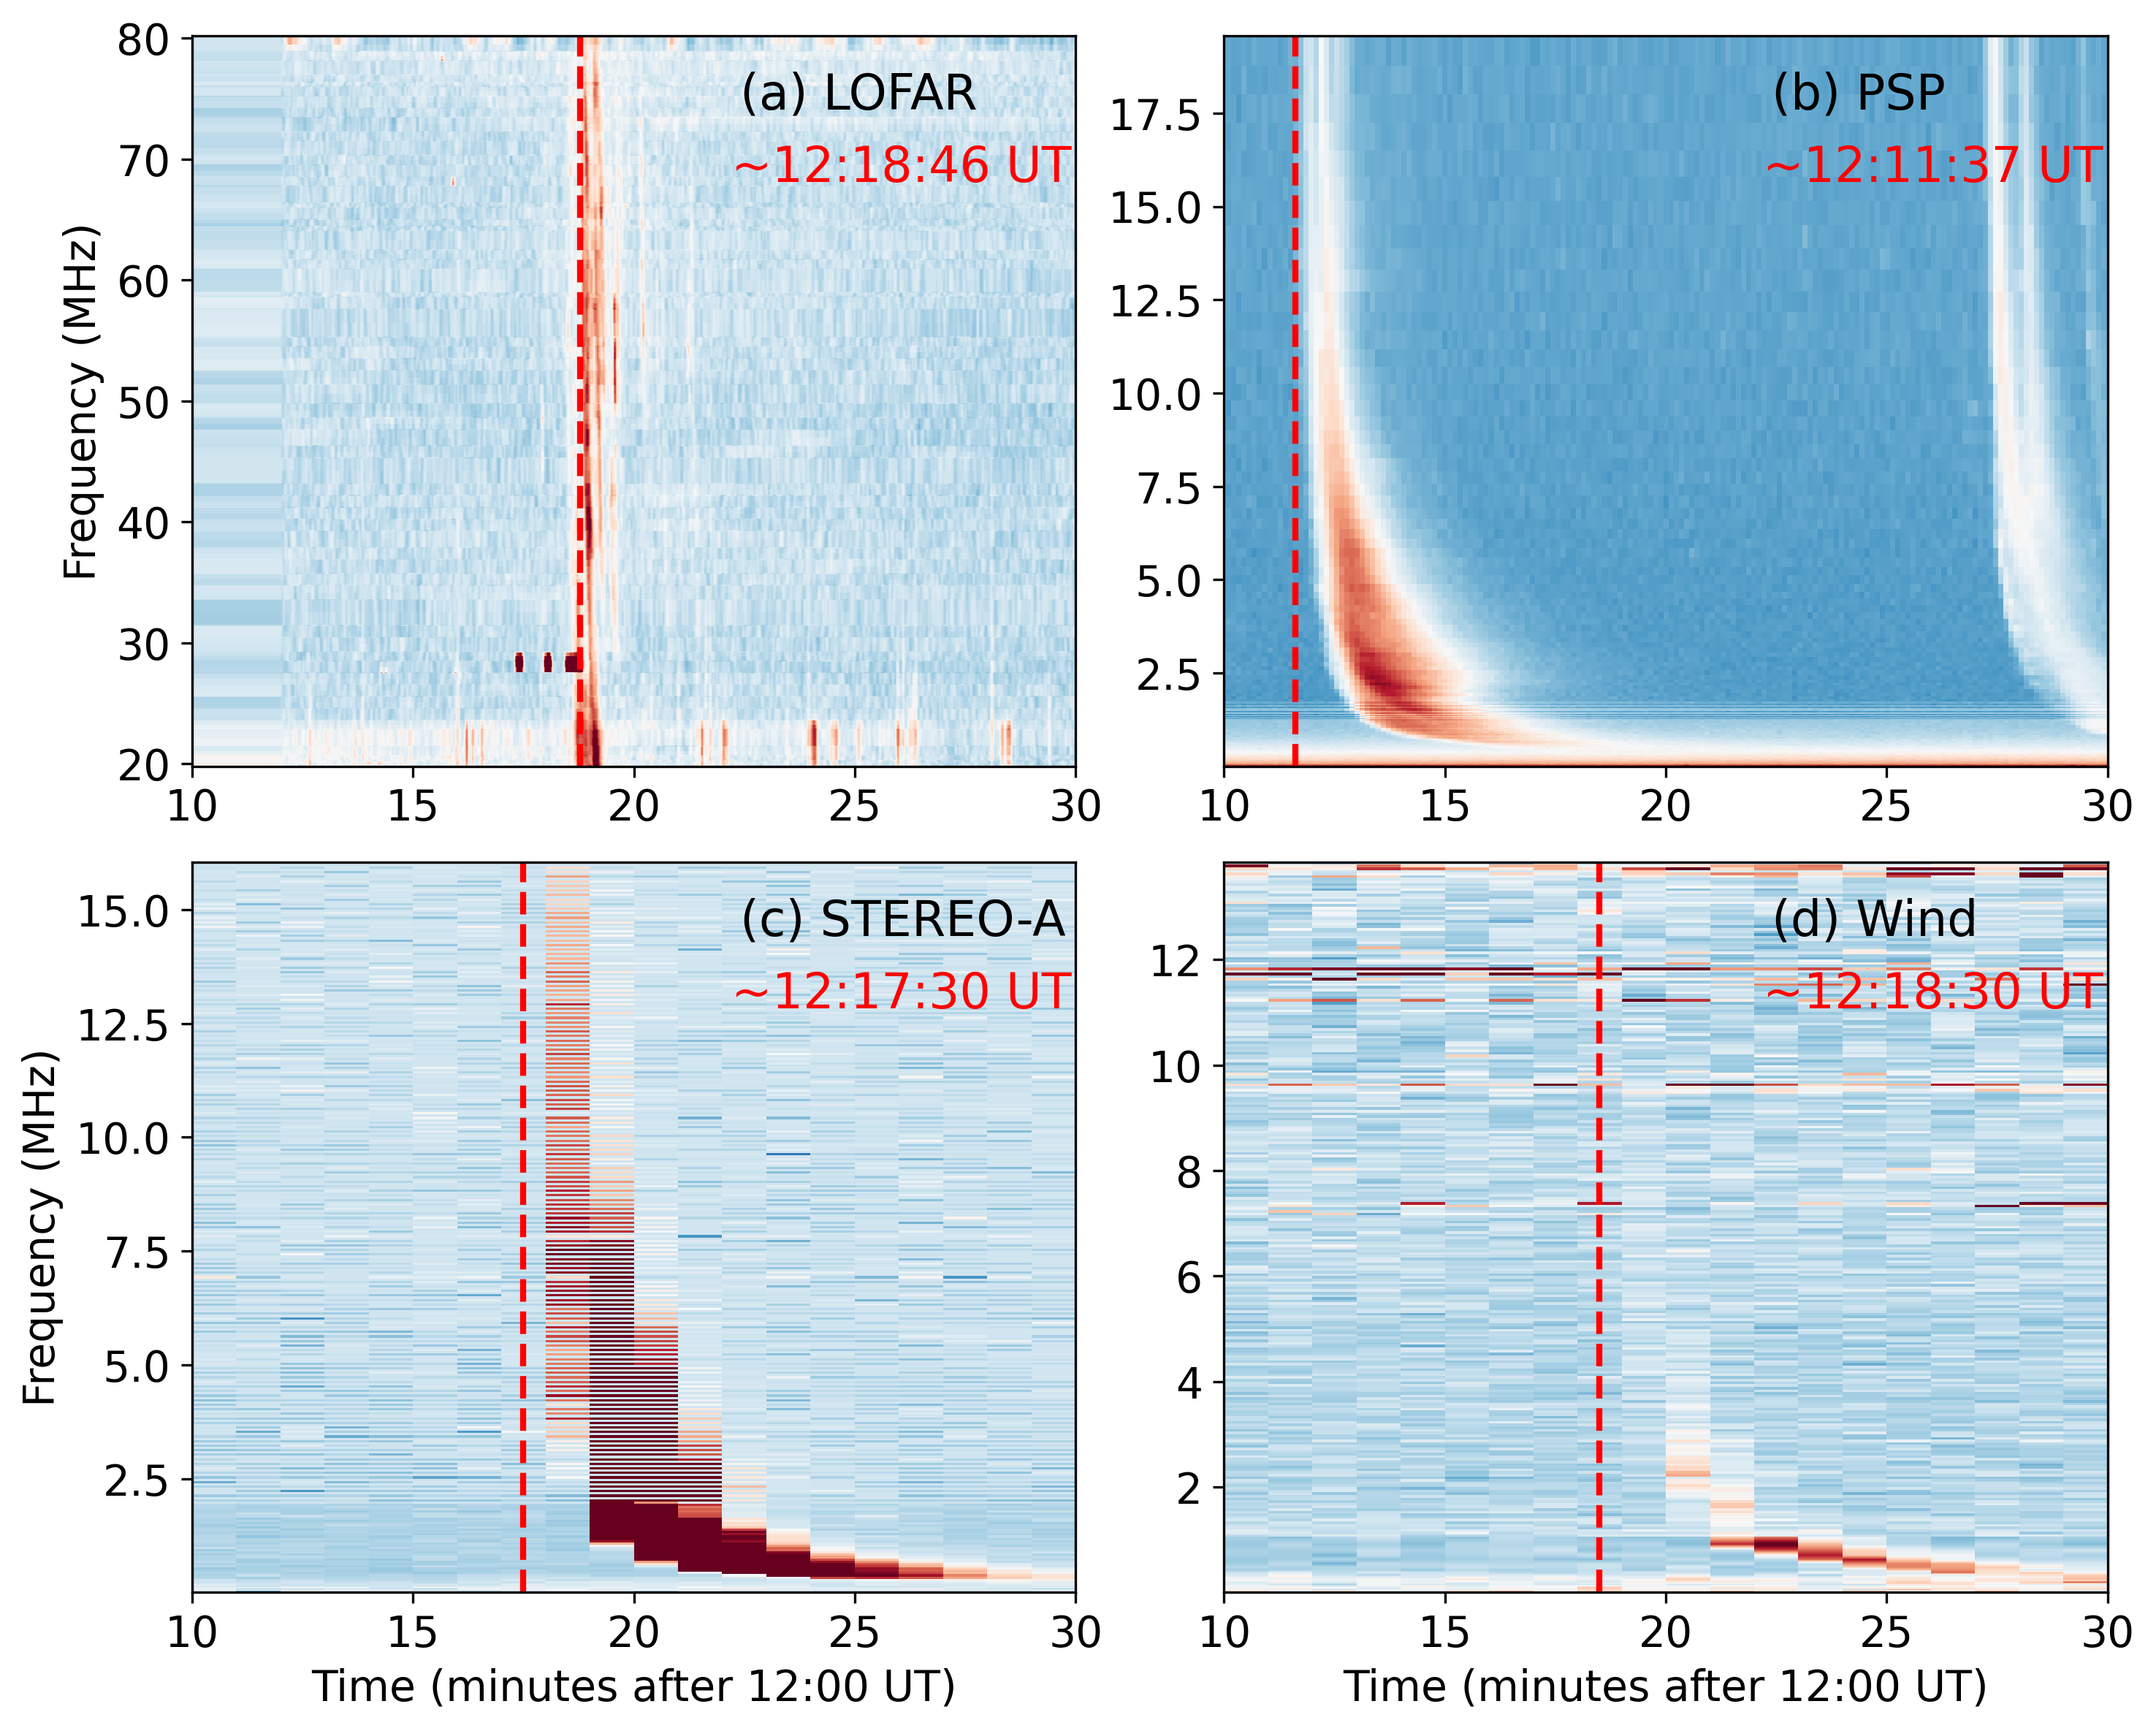
\includegraphics[width=0.9\hsize]{chapter2/figs/all_dyspec.png}
\caption{Radio dynamic spectra for a single burst obtained from multiple instruments. The top-left panel is from the LOFAR/LBA instrument, the top-right is from the PSP/FIELDS instrument, the bottom-left is from the STEREO/SWAVES instrument, and the bottom-right is from the Wind/WAVES. The vertical red dashed line denotes the start time of the burst.}
\label{fig_alldyspec}
\end{figure}

\begin{figure}
\centering
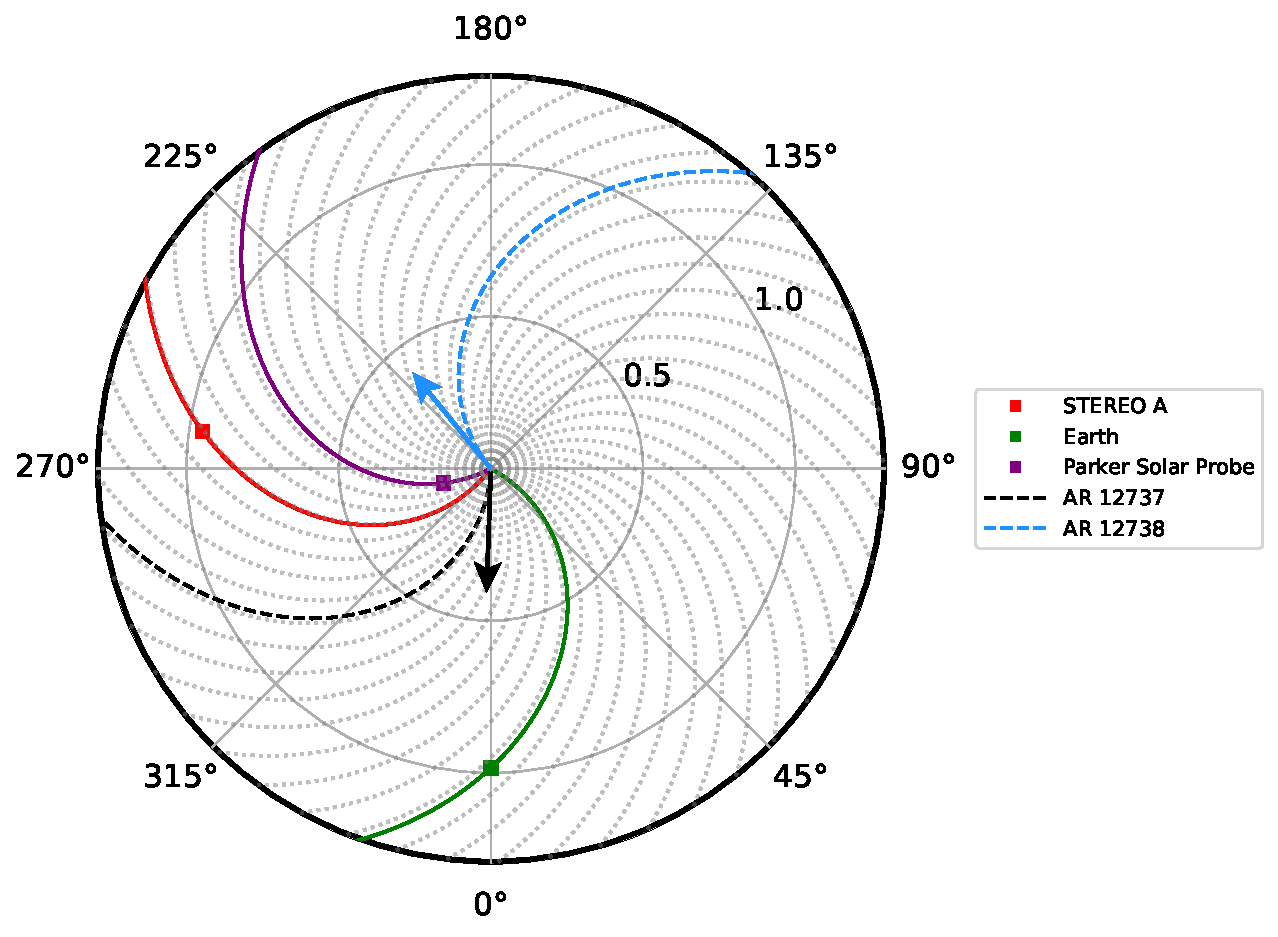
\includegraphics[width=0.8\hsize]{chapter2/figs/solarMach.pdf}
  \caption{Top view of the spacecraft positions in the ecliptic plane at 12:15 UT on April 3, 2019, with the Sun-Earth line as the reference point for longitude. The Earth's location is representative of the positions of LOFAR, Wind/WAVES, and GOES-15/XRS instruments. The spacecraft were connected back to the Sun by a 400 km/s reference Parker Spiral. The black arrow represents the longitude of AR12737 and the blue arrow represents the longitude of the AR12738. The gray dotted lines are the background Parker spiral field lines. The black dashed spiral shows the field line connected to the AR12737, and the blue dashed spiral is connected to the AR12738. The figure is generated using the Solar MAgnetic Connection Haus (\href{https://github.com/jgieseler/solarmach}{Solar-MACH}) tool \citep{Gieseler2023}.}
     \label{locations}
\end{figure}

\begin{figure*}[ht]
\centering
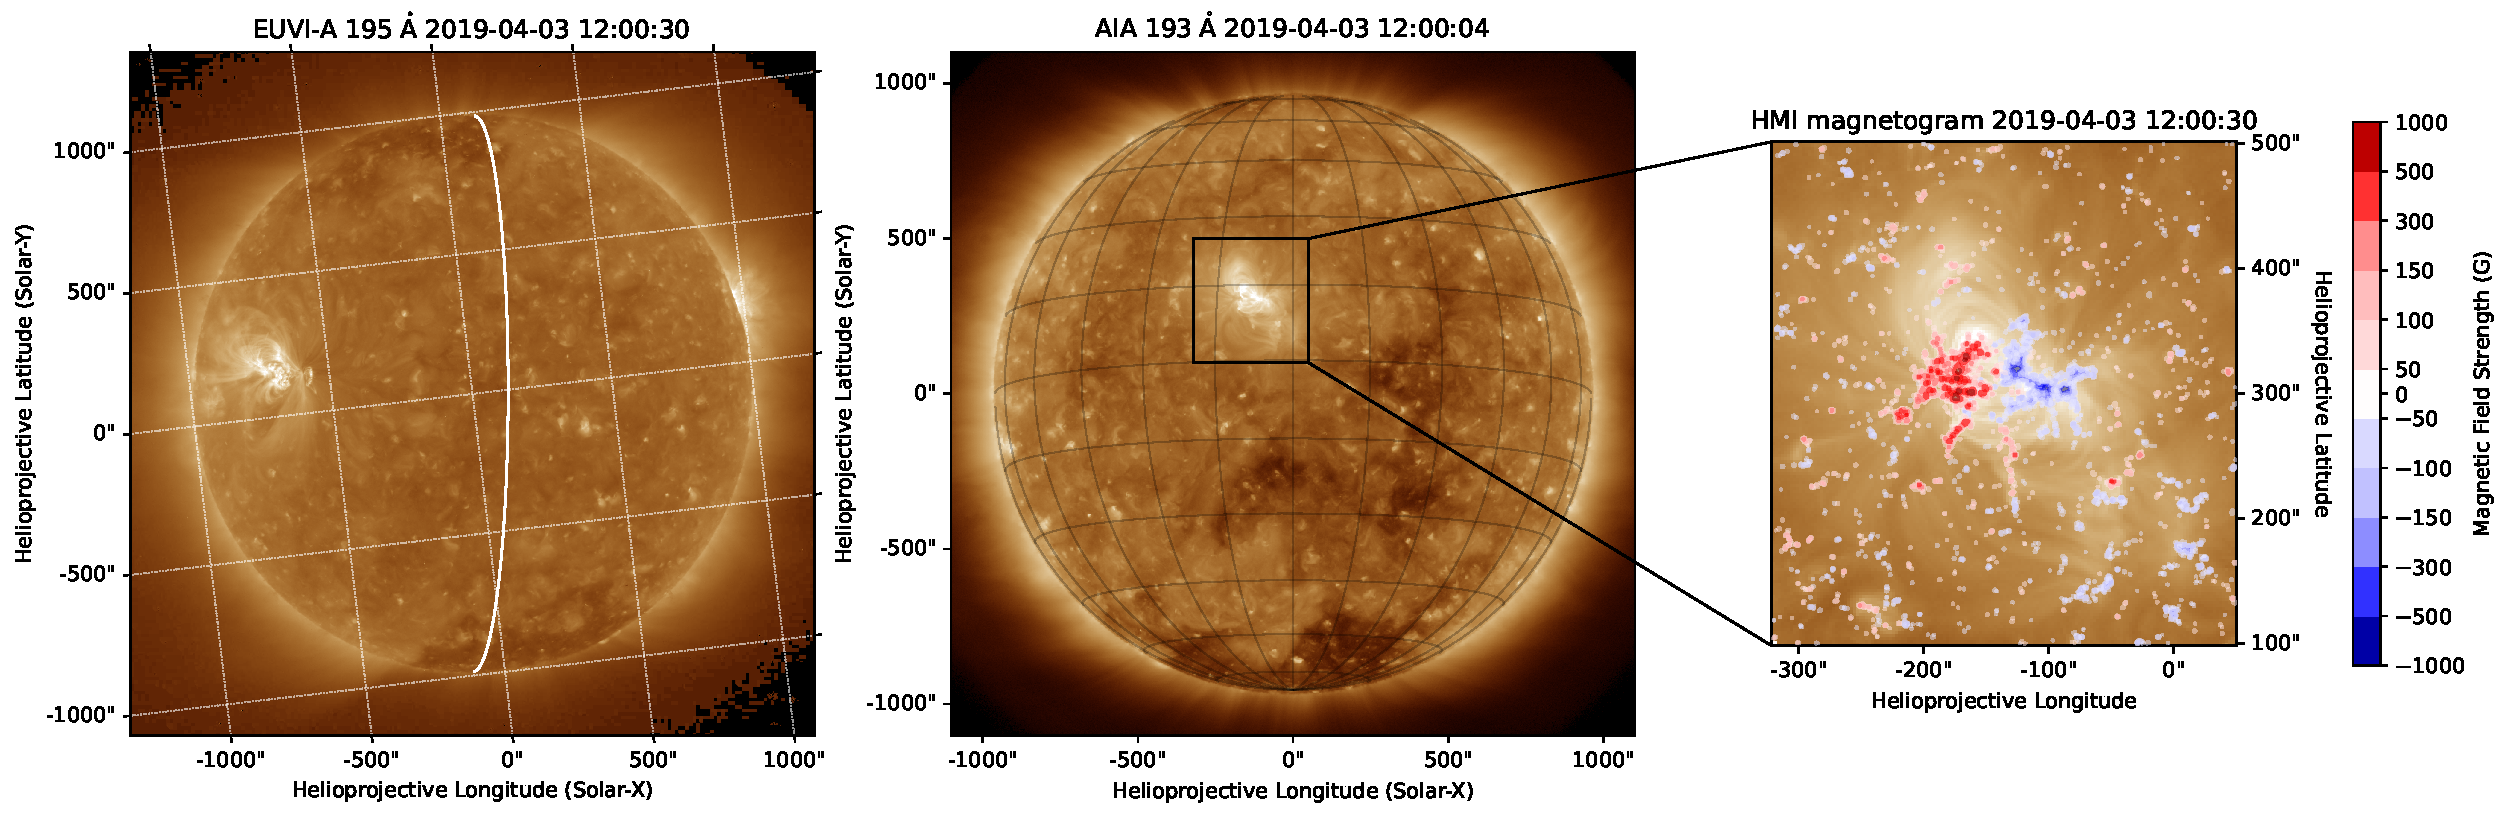
\includegraphics[width=\hsize]{chapter2/figs/aia_sta_cutout.pdf}
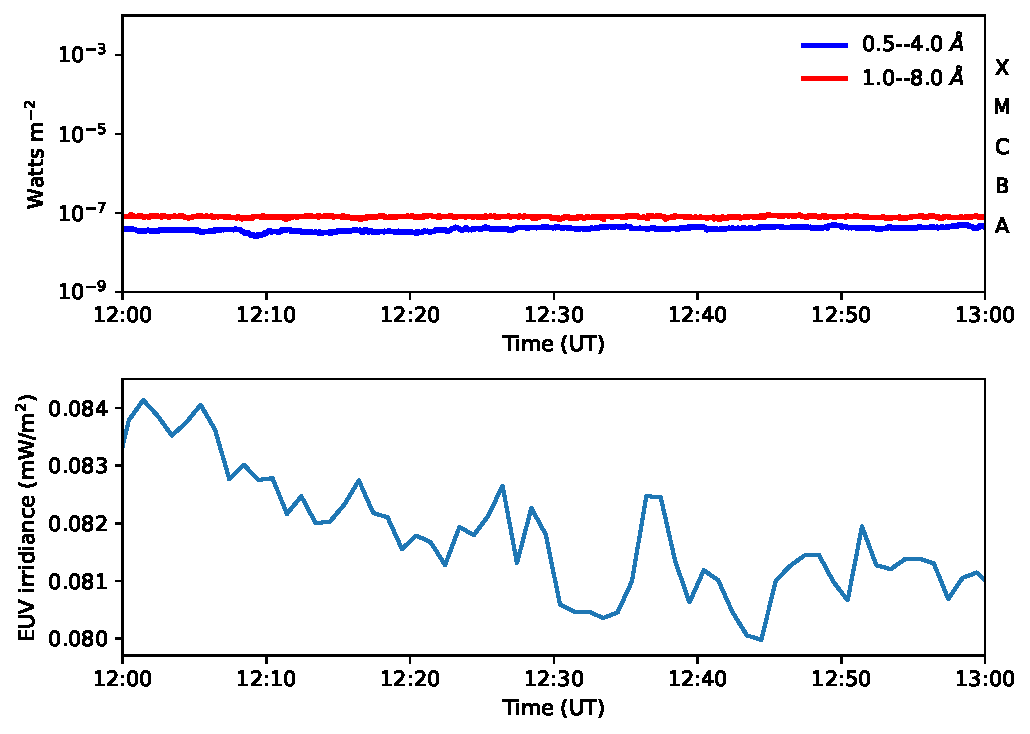
\includegraphics[width=12cm]{chapter2/figs/xrs_eve.pdf}
\caption{Exploring the X-ray and extreme ultraviolet (EUV) emissions from the Sun. The top panel showcases a cutout region of the SDO/AIA 193\,\AA image of the solar disk along with the STEREO-A EUVI 195\,\AA point of view. The white curve is the limb of the solar disk as seen by AIA from the right side. The red and blue colors are the contours of the line-of-sight magnetogram from the SDO/HMI instrument. The levels are (50, 100, 150, 300, 500, 1000) Gauss. The middle panel shows the X-ray flux from the GOES-14 spacecraft shows minimum activity. The bottom panel shows the time series of the ESP Quad band from the SDO/EVE instrument, which shows the solar irradiance in the extreme ultraviolet (EUV) band.}
\label{soldisk_xrs}
\end{figure*}

\subsection{PSP Observations}

\subsection{LOFAR Observations}


\section{Methods}

\subsection{Imaging of radio sources}

\subsection{Modeling}


\section{Results and discussion}

\subsection{Detection and characterization of type III radio bursts}

\subsection{Imaging of radio emission sources}

\subsection{Plasma diagnostics and magnetic field analysis}


\section{Summary and conclusions}



	\chapter{Modeling and Foreasting Solar Energetic Protons (SEP)}
\label{chapter3}

\section{Introduction}

\section{Data preparation}

\section{Method}

\subsection{The Bi-LSTM Model}

\subsection{Model selection}


\section{Results and discussion}

\section{Conclusions}



	\chapter{Modeling and Forecasting of Solar Energetic Protons (SEP)}
\label{chapter4}

\section{Introduction}
\label{sec_ch4_intro}
Several models are available, or under development, for forecasting SEP, which use diverse approaches and serve different objectives. These models comprise computationally complex physics-based models, quick and simple empirical models, Machine Learning (ML)-based models, and hybrid models that combine different approaches and produce different types of outputs, including deterministic, probabilistic, categorical, and binary. Deterministic models always generate the same output without any randomness or stochastic components, such as predicting the SEP flux at a specific moment or the arrival time of SEP. On the other hand, probabilistic models provide a probability value that reflects the likelihood of an SEP event occurring. However, replicating SEP fluxes at a specific time is still a significant challenge for current models.

An excellent review on SEP models and predictive efforts was recently published by \citet{whitman_2022}, which summarizes the majority of the existing models.
For instance, \citet{papaioannou_2022} introduced the Probabilistic Solar Particle Event Forecasting (PROSPER) model, which is incorporated into the Advanced Solar Particle Event Casting System (ASPECS)\footnote{\url{http://phobos-srv.space.noa.gr/}}. The PROSPER model utilizes a Bayesian approach and data-driven methodology to probabilistically predict SEP events for 3 integral energy channels $>$10, $>$30, and $>$100 MeV. The model's validation results indicate that the solar flare and CME modules have hit rates of 90\% and 100\%, respectively, while the combined flare and CME module has a hit rate of 100\%.
\citet{bruno_2021} developed an empirical model to predict the peak intensity and spectra of SEP at 1 AU between 10 and 130 MeV, using data from multiple spacecraft. The model is tested on 20 SEP events and shows good agreement with observed values. The spatial distribution of SEP intensities was reconstructed successfully, and they found a correlation between SEP intensities and CME speed.
%%% briefly mention the physics-based models ...
\citet{hu_2017} extended the Particle Acceleration and Transport in the Heliosphere (PATH) model to study particle acceleration and transport at CME-driven shocks. They showed that the model can be used to obtain simultaneous calculations of SEP characteristics such as time-intensity profiles, instantaneous particle spectra, and particle pitch angle distributions at multiple heliospheric locations. Overall, results resemble closely those observed in situ near the Earth but also yield results at other places of interest, such as Mars, making it of particular interest to Mars missions.
SPREAdFAST \citep{kozarev_2017, kozarev_2022} is a physics-based, data-driven framework that utilizes EUV observations and models to simulate SEP fluxes at 1 AU and to estimate energetic particle acceleration and transport to various locations in the inner heliosphere. It generates time-dependent histograms and movies distributing them through an online catalog. The accuracy and efficiency of the model were encouraging, but the highest energy fluxes showed disagreement with in situ observations by the SOHO/ERNE instrument. However, the framework has great potential for space weather science and forecasting.

In \citet{aminalragia_2021}, they used neural networks to provide probabilities for the occurrence of SEP based on soft X-rays data from 1988 to 2013. They obtained $>$85\% for correct SEP occurrence predictions and $>$92\% for correct no-SEP predictions.
\citet{lavasa_2021} described a consistent approach to making a binary prediction of SEP events using ML and conventional statistical techniques. The study evaluated various ML models and concluded that random forests could be the best approach for an optimal sample comprising both flares and CMEs. The most important features for identifying SEP were found to be the CME speed, width, and flare soft X-ray fluence.
\citet{kasapis_2022} employed ML techniques to anticipate the occurrence of a SEP event in an active region that generates flares. They utilized the Space-Weather MDI Active Region Patches (SMARP) dataset, which comprises observations of solar magnetograms between June 1996 and August 2010. The SMARP dataset had a success rate of 72\% in accurately predicting whether an active region that produces a flare would result in a SEP event. Moreover, it provided a competitive lead time of 55.3 min in forecasting SEP events.

\citet{engell_2017} introduced the Space Radiation Intelligence System (SPRINTS), a technology that uses pre- and post-event data to forecast solar-driven events such as SEP. It integrates automatic detections and ML to produce forecasts. Results show that SPRINTS can predict SEP with an 56\% probability of detection and 34\% false alarm rate.
Nevertheless, the HESPERIA REleASE tools provide real-time predictions of the proton flux at L1 by using near-relativistic electrons as a warning for the later arrival of protons and have been set to operation\citep{malandraki_2018}. Historical data analysis indicates high prediction accuracy, with a low false alarm rate of approximately 30\% and a high probability of detection of 63\% \citep{malandraki_2018}.

Forecasting SEP is a critical task that serves operational needs and provides insight into the broader field of space weather science and heliophysics. As emphasized in previous works, a high precision forecasting model is urgently required to predict SEP flux within a period of time, given the risks associated with these events. This highlights the critical requirement for a dependable forecasting system that can mitigate the risks associated with SEP.

Scientists have been using physics-based and empirical models for decades to forecast SEP. However, these models have certain limitations. Physics-based models require accurate input data and underlying physical assumptions. In addition, the complexity of the physics involved and incorrect parameters may introduce uncertainties that can lead to inaccurate predictions.
On the other hand, empirical models rely on historical data to make predictions.
While they can be accurate sometimes, they may be unable to account for changes in physical conditions related to the acceleration and propagation of SEP, which can influence prediction accuracy.
ML models, however, provide a different approach to SEP forecasting. These models can analyze vast amounts of data, learning patterns from the data that are used, and connections that may not be obvious to experts. Additionally, ML models can adapt to changes in underlying physical conditions, resulting in more accurate predictions as more data is collected; they also provide relatively rapid forecasts, which allows for incorporation into a real-time forecasting workflow.

In the upcoming sections, we will explore the limitations in accuracy that arise from dealing with an imbalanced dataset and low-resolution data. Specifically, the presence of intrinsic outliers in the time series data pertaining to SEP flux poses a significant challenge in modeling. These outliers correspond to occurrences of SEP events and, consequently, have an impact on the accuracy of predictions. Notably, they often lead to an underestimation of the SEP fluxes, primarily due to the predominance of relatively low values throughout the majority of the time interval.

In this paper, we present advanced deep learning models to forecast the daily integral flux of SEP over a 3-day forecasting window by using bi-directional long short-term memory (BiLSTM) neural networks, for 3 energy channels ($>$10, $>$30, and $>$60 MeV).
Our models can forecast the time-dependent development of SEP events in different energy domains, which can be used to model the space radiation profiles using frameworks such as BRYNTRN \cite{wilson_1988} and GEANT4 \citep{truscott_2000}.
We describe the data selection and pre-processing in Section~\ref{sec_ch4_data_prep}. We present an overview on the analysis methods and the models implemented in Section~\ref{sec_ch4_methods}. Then we show the forecasting results in Section~\ref{sec_ch4_results}. Finally the summary and implications are presented in Section~\ref{sec_ch4_conclusion}.

\section{Data preparation}
\label{sec_ch4_data_prep}
In this section, we describe the physical quantities, the types of inputs and their sources, as well as the outputs we are forecasting.
Some of the technical terms used in this study are explained further in the appendices.

In order to capture the variability of solar activity, which modulates the SEP flux, we selected input physical quantities that describe both the interplanetary medium and solar activity. These input features can be categorized into two groups: remote signatures and in-situ measurements.
The remote signatures consist of the F10.7 index, as well as the long-wavelength ($X_L$) and short-wavelength ($X_S$) x-ray fluxes. The F10.7 index represents the flux of solar radio emission at a wavelength of 10.7 cm, measured in solar flux units (sfu). To obtain the x-ray fluxes, we utilized 1- and 5-minute averaged data from the Geostationary Operational Environmental Satellite (GOES) database\footnote{\url{https://satdat.ngdc.noaa.gov/sem/goes/data/avg/}}, specifically at long wavelengths (1 - 8 \AA) and short wavelengths (0.5 - 4.0 \AA).

The in-situ measurements encompass the near-Earth solar wind magnetic field and plasma parameters. These include the solar wind speed (in km s$^{-1}$), average interplanetary magnetic field (IMF) strength (in nT), and the integral SEP fluxes at three energy channels: $>$10, $>$30, and $>$60 MeV, which correspond to the GOES channels (in 1/cm$^2$ sec ster). These SEP fluxes were obtained from multiple spacecraft stationed at the first Lagrange point (L1) throughout the study period.
In particular, the IMF and plasma data in the OMNI database are obtained from the IMP, Wind, and ACE missions, while the energetic particle fluxes are obtained from the IMP and GOES spacecraft\footnote{\url{https://omniweb.gsfc.nasa.gov/html/ow_data.html}}.

To ensure a comprehensive dataset, we acquired hourly-averaged data covering a timeframe from December 1976 to July 2019, which spans the past four solar cycles. These data were sourced from the Space Physics Data Facility (SPDF) OMNIWeb database\footnote{\url{https://omniweb.gsfc.nasa.gov}}, hosted by the Goddard Space Flight Center. This database provides a wealth of information, including integral proton fluxes, as well as an extensive range of solar wind plasma and magnetic field parameters.
Lastly, the daily data on sunspot numbers were obtained from the Sunspot Index and Long-term Solar Observations (SILSO) archive\footnote{\url{https://www.sidc.be/silso/home}}, maintained by the World Data Center.

Figure~\ref{fig_allFeatures} shows a plot for the timeseries data of all features.
The top 3 panels are the logarithms of the SEP integral flux at the 3 energy channels (log\_PF10, log\_PF30, and log\_PF60), then the sunspot number, the F10.7 index (F10\_idx), the logarithms of the x-ray fluxes (log\_Xs and log\_Xl), the solar wind speed (Vsw), and the average magnitude of the IMF (avg\_IMF).
Throughout this paper, we adopt the convention that "log" refers to the common logarithm with a base of 10.
The gray shades refer to the timespan of solar cycles.
The blue, orange, and gold colors refer to the training, validation, and test sets, respectively. The data split method will be explained shortly.

Since the input SEP data have been compiled from various spacecraft, it may have artifacts even after processing. In particular, there are occasional jumps in the background level. There are also several day-long gaps in the OMNI solar wind parameters from the early 1980s to mid-1990s where only IMP 8 data are available and this spacecraft spent part of each orbit in the magnetosphere. We are reasonably confident that these issues do not influence the overall analysis significantly.

In deep learning applications, the dataset is split into 3 sets; namely the training set, the validation set, and the test set. The training set is usually the largest chunk of data that is used to fit the model. The validation set is a smaller chunk of data used to fine-tune the model and evaluate its accuracy to ensure it is unbiased. The test set is the out-of-sample data exclusively used to assess the final model when performing on unseen data \citep{ripley_2007}.

After inspecting the correlation between the solar wind indices and the SEP integral fluxes in the OMNIWeb database, we chose the top-correlated features with the SEP flux. The correlations were made between the SEP fluxes and the individual parameters. Hence we took only timeseries of logarithms of the protons' integral flux at 3 energy channels ($>$10, $>$30, and $>$60 MeV), the timeseries of logarithm of the X-ray fluxes, the F10.7 index, the sunspot number, the solar wind speed, and the average strength of the IMF as input parameters to our model.
The log of the SEP flux was used across the whole study.
The correlation matrices for the training, validation, and test sets are shown in Figure~\ref{fig_dataCorr}.
The X-ray and proton fluxes were converted into the logarithmic form because it was more convenient than the original form of data since the time series data were mostly quiet and had numerous sharp spikes, which correspond to solar events.
Based on a previous experience with NNs \citep{mnedal_2019}, we found that training separate models for each target (output) feature can lead to better results. This is because a dedicated model for each  output feature can more easily learn the interrelationships between input features and make more accurate predictions. Therefore, in our current study, we trained 3 separate models, each one targeting the logarithm of the protons integral flux at a specific energy channel.

In order to ensure consistency across all features, all durations of the time series data of the physical quantities were matched to be within the same time range. Subsequently, the dataset was resampled to obtain daily averaged data, resulting in a significant reduction of the dataset size by a factor of 24. This reduction facilitated expeditious training and yielded prompt results.

There were missing data values in the original dataset; for the $B_{avg}$ ($\sim$10.7\%), $V_{sw}$ ($\sim$10.5\%), F10.7-index ($\sim$0.08\%), short-band x-ray flux ($\sim$8\%), long-band x-ray flux ($\sim$9.8\%), and proton fluxes ($\sim$4.3\%). The data gaps were linearly interpolated.

\begin{figure}[h!]
    \centerline{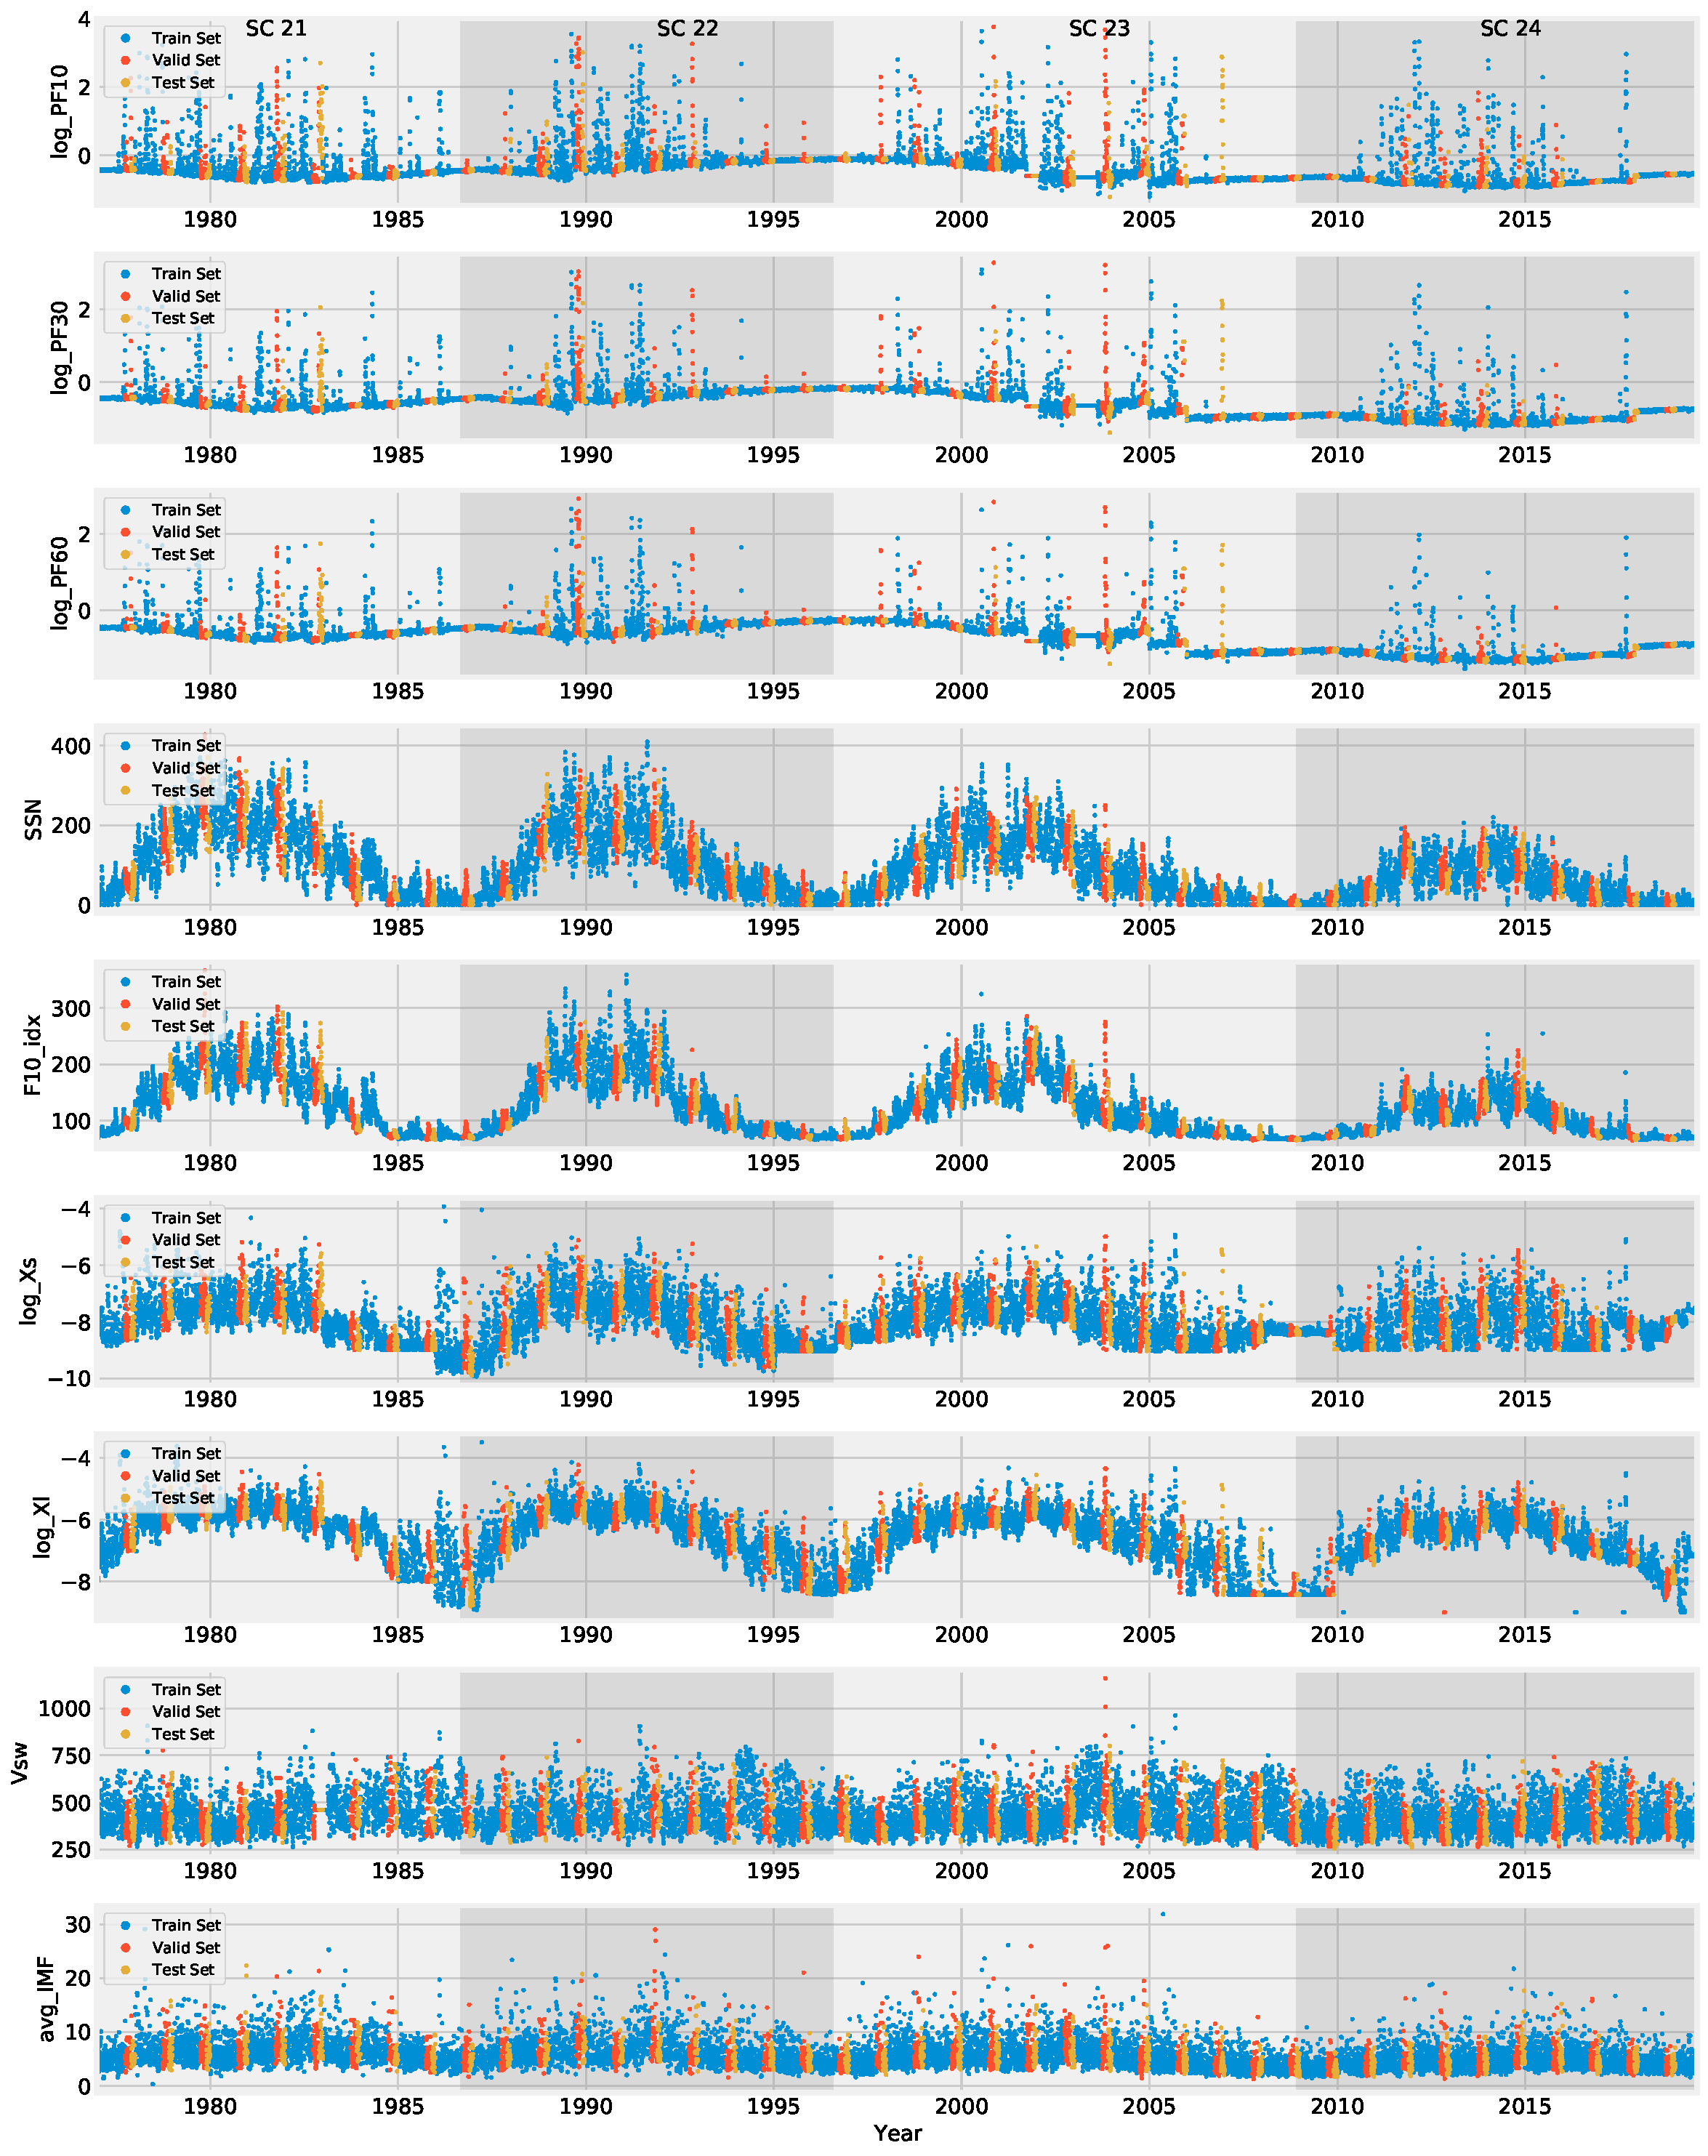
\includegraphics[width=0.9\textwidth]{chapter4/figs/subplots_dataSplit_allFeatures.pdf}}
    \caption{Data splitting for all input features, showing the training, validation, and testing sets. Daily data from 1976-12-25 00:00 to 2019-07-30 00:00. The gray shading labels the solar cycles from SC21 to SC24.}
\label{fig_allFeatures}
\end{figure}

In timeseries forecasting, it is a common practise to take a continuous set of data points from the main dataset to be the validation set and another smaller chunk of data to be the test set, for instance in \citet{pala_2019, benson_2020, zhang_2022, zhu_2022}. 
From our experiments, we got descent results when we applied the same data split method, but the results were a bit biased toward the end of the solar cycle 24 and the testing set was biased towards a quiet period. So, we adopted the 9-2-1 strategy, that is taking from each year 9 months to be added in the training set, 2 months to be added in the validation set, and 1 month to be added in the test set. This is applied over the $\sim$43 years of data (Fig.~\ref{fig_allFeatures}), which yields 74.29\% of the data for the training set, 16.2\% for the validation set, and 9.51\% for the testing set. By doing so, we eliminated the need to do cross-validation and hence, made the training more efficient.
It is worth to mention that the timeseries data must not be shuffled as that will break temporal and logical order of measurements, which must be maintained.

\begin{figure}[htp]
    \centerline{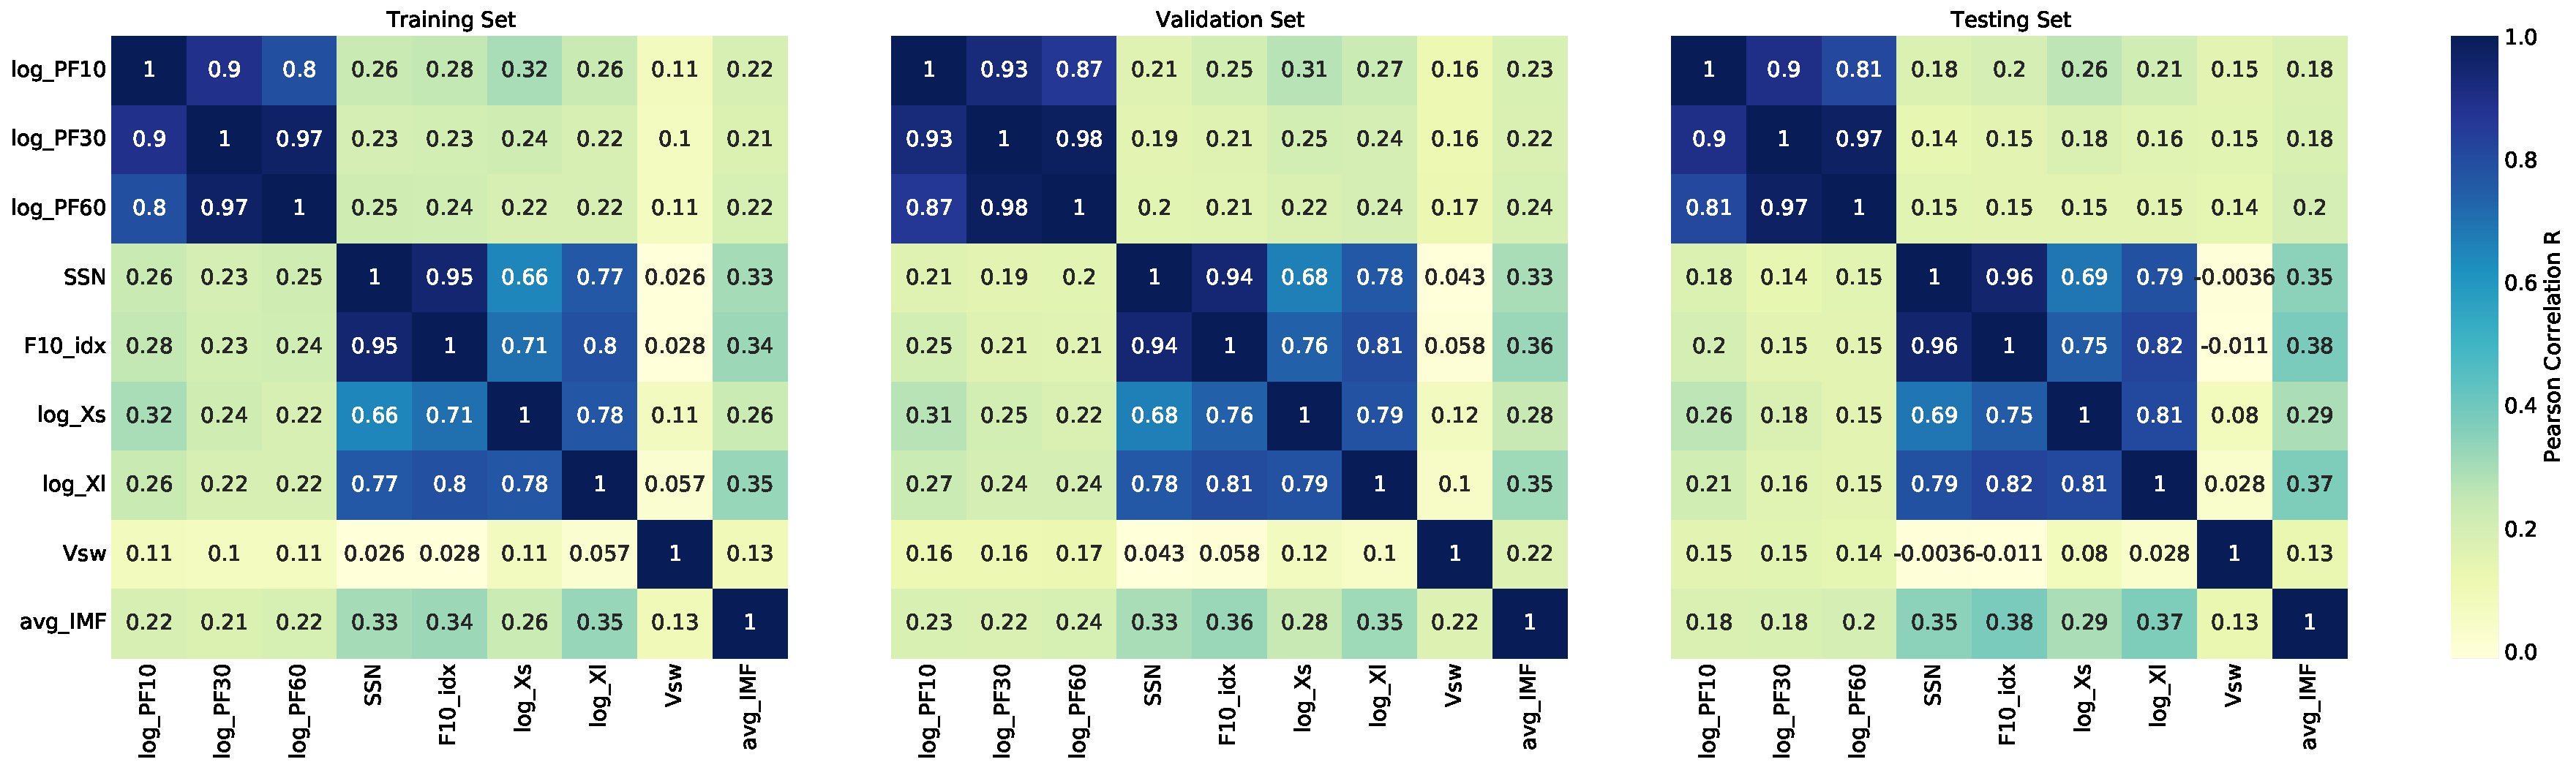
\includegraphics[width=\textwidth]{chapter4/figs/dataset_split_corr.pdf}}
    \caption{Correlation matrices show the correlation between the features in the training, validation, and test sets.}
\label{fig_dataCorr}
\end{figure}

\section{Method}
\label{sec_ch4_methods}
In this section, we introduce the data analysis methods used in this work. We start with explaining the model selection phase, followed by a discussion of the bidirectional long-short-term memory (BiLSTM) neural network architecture. The technical terminologies are described in the appendices.

\subsection{The Bi-LSTM Model}
Recurrent neural networks (RNNs) that support processing input sequences both forward and backward are known as Bidirectional Long Short-Term Memory (BiLSTM) neural networks \citep{schuster_1997}. Regular RNNs \citep{hochreiter_1997, kolen_2001} depend on the prior hidden state and the current input to determine the output at a given time. The output of a BiLSTM network, on the other hand, is dependent on the input at a given moment as well as the previous and future hidden states. As a result, the network is able to make predictions using contexts from the past as well as the future. Hence, accuracy is improving.
Each BiLSTM layer consists of two LSTM layers; a forward layer that processes the input sequences from the past to future, and a backward layer that processes the input sequences from the future to the past, as illustrated in Figure~\ref{fig_model}, to capture information from both past and future contexts. The output from each layer is concatenated and fed to the next layer, which can be another BiLSTM layer or a fully connected layer for final prediction.

BiLSTM networks are advantageous than traditional LSTM networks in a variety of aspects \citep{graves_2005, ihianle_2020, alharbi_2021}. First, as we demonstrate in this study, they are excellent for tasks like timeseries forecasting, as well as speech recognition and language translation \citep{wollmer_2013, graves_2014, sundermeyer_2014, huang_2018, nammous_2022} because they can capture long-term dependencies in the input sequence in both forward and backward directions. Second, unlike feedforward networks, BiLSTM networks do not demand fixed-length input sequences, thus being able to handle variable-length sequences better. Furthermore, by taking into account both past and future contexts, BiLSTM networks can handle noisy data.
However, BiLSTM networks are computationally more expensive than regular LSTM networks due to the need for processing the input sequence in both directions. They also have a higher number of parameters and require more training data to achieve good performance.

\begin{figure}[htp]
    \centerline{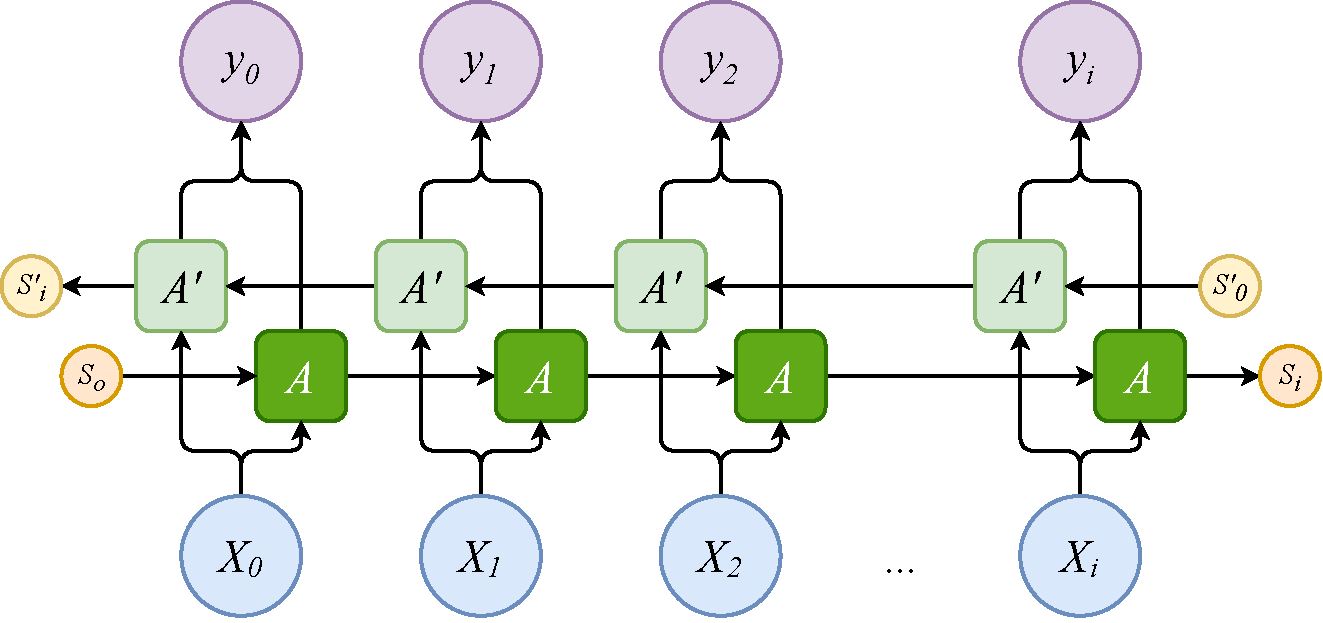
\includegraphics[width=0.6\textwidth]{chapter4/figs/diagram.drawio.pdf}}
    \caption{Architecture of a single BiLSTM layer. The blue circles at the bottom labeled by \textit{($x_0$, $x_1$, $x_2$, ..., $x_i$)} are the input data values at multiple time steps. The purple circles, on the other hand, are the output data values at multiple time steps labeled by \textit{($y_0$, $y_1$, $y_2$, ..., $y_i$)}. The dark green and light green boxes are the activation units of the forward layer and the backward layer, respectively. The orange and yellow circles are the hidden states at the forward layer and the backward layer, respectively. Both the forward and backward layers composes a single hidden BiLSTM layer. The figure is adopted from \citet{olah_2015}}
\label{fig_model}
\end{figure}

The final dataset has 7 features, including the target feature, from December 25$^{th}$ 1976 to July 30$^{th}$ 2019, with a total of 15,558 samples (number of days). The training set has 11,558 samples, the validation set has 2,520 samples, and the test set has 1,480 samples.

The input horizon of 270 steps (30 days × 9 months) was used.
A data batch size of 30 was used, which is the number of samples processed that result in one update to the model's weights (Appendix~\ref{bilstm_appendix}).
The model consists of 4 BiLSTM layers with 64 neurons each, and an output dense layer with 3 neurons, representing the output forecasting horizon.
The total number of trainable parameters is 333,699.
The number of training epochs was set to 50 because from experiments, the model stopped improving remarkably after almost 50 epochs. Thus, there was no need to waste time and computational resources to train the model for more than 50 epochs.

The \textit{ModelCheckpoint} callback function was used to register the model version with the minimal validation loss. 
The \textit{EarlyStopping} callback function was used to halt the model run when detecting overfitting, with a \textit{patience} parameter of 7. 
\textit{ReduceLROnPlateau} callback function was used to reduce the learning rate when the validation loss stops improving, with a \textit{patience} parameter of 5, a reduction factor of 0.1 and minimal learning rate of 1e$^{-6}$.
% ---------------------------------------------------------------
\subsection{Model Selection}
To determine the most suitable model for our objective and provide justifiable reasons, we conducted the following analysis.
First we examined the naive (persistence) model, which is very simplistic and assumes that the timeseries values will remain constant in the future. In other words, it assumes that the future value will be the same as the most recent historical value. That was the baseline. Next we examined the moving-average model, which calculates the future values based on the average value of historical data within a specific time widow. This gives a little bit lower error.

\begin{figure}[htp]
    \centerline{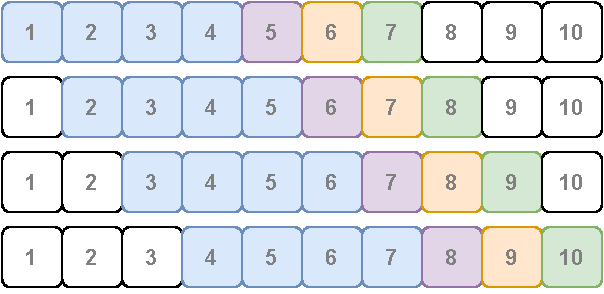
\includegraphics[width=0.5\textwidth]{chapter4/figs/sliding_window_lstm.pdf}}
    \caption{Illustration of the sliding window technique for a sample of 10 timesteps, where each number denotes a distinct time step. As an example here, the input horizon (blue color) length is 4 timesteps and the output horizon length is 3 timesteps. The input window slides 1 time step at a time across the entire data sequence to generate 4 distinct input and forecast horizon pairs. The purple, orange, and green colors of the output horizon represent 1-day, 2-day, and 3-day ahead forecasting, respectively. The timesteps of 1-day ahead forecasting across the data sequences are then concatenated into a single timeseries list that is called 1-day ahead prediction. The same for 2-day and 3-day ahead.}
\label{fig_slide_window}
\end{figure}

After that, we went towards the machine learning (ML)-based models. For all the ML models, we chose the Adaptive moment estimation (Adam) optimizer \citep{kingma_2015} as the optimization algorithm due to its minimal memory requirements and high computational efficiency as it is well-suited for applications that involve large number of parameters or large datasets. As a rule of thumb, we set the optimizer’s learning rate to be 0.001 as it is usually recommended \citep{zhang_2022}.

In order to prepare the data in a readable format to the ML models, we created a windowed dataset with an input horizon of 365 steps representing 1 year of data and an output horizon of 3 steps representing the forecast window of three days. We call this windowing method as Multi-Input Multiple Output (MIMO) strategy, in which the entire output sequence is predicted in one shot. The MIMO strategy adopts the sliding window method that was mentioned in \citet{benson_2020} in which each sequence is shifted by one step with respect to the previous sequence until reaching the end of the available data (Fig.~\ref{fig_slide_window}).
This approach minimized the imbalance of active days, with high SEP fluxes, and quiet days.

\begin{figure}[htp]
    \centerline{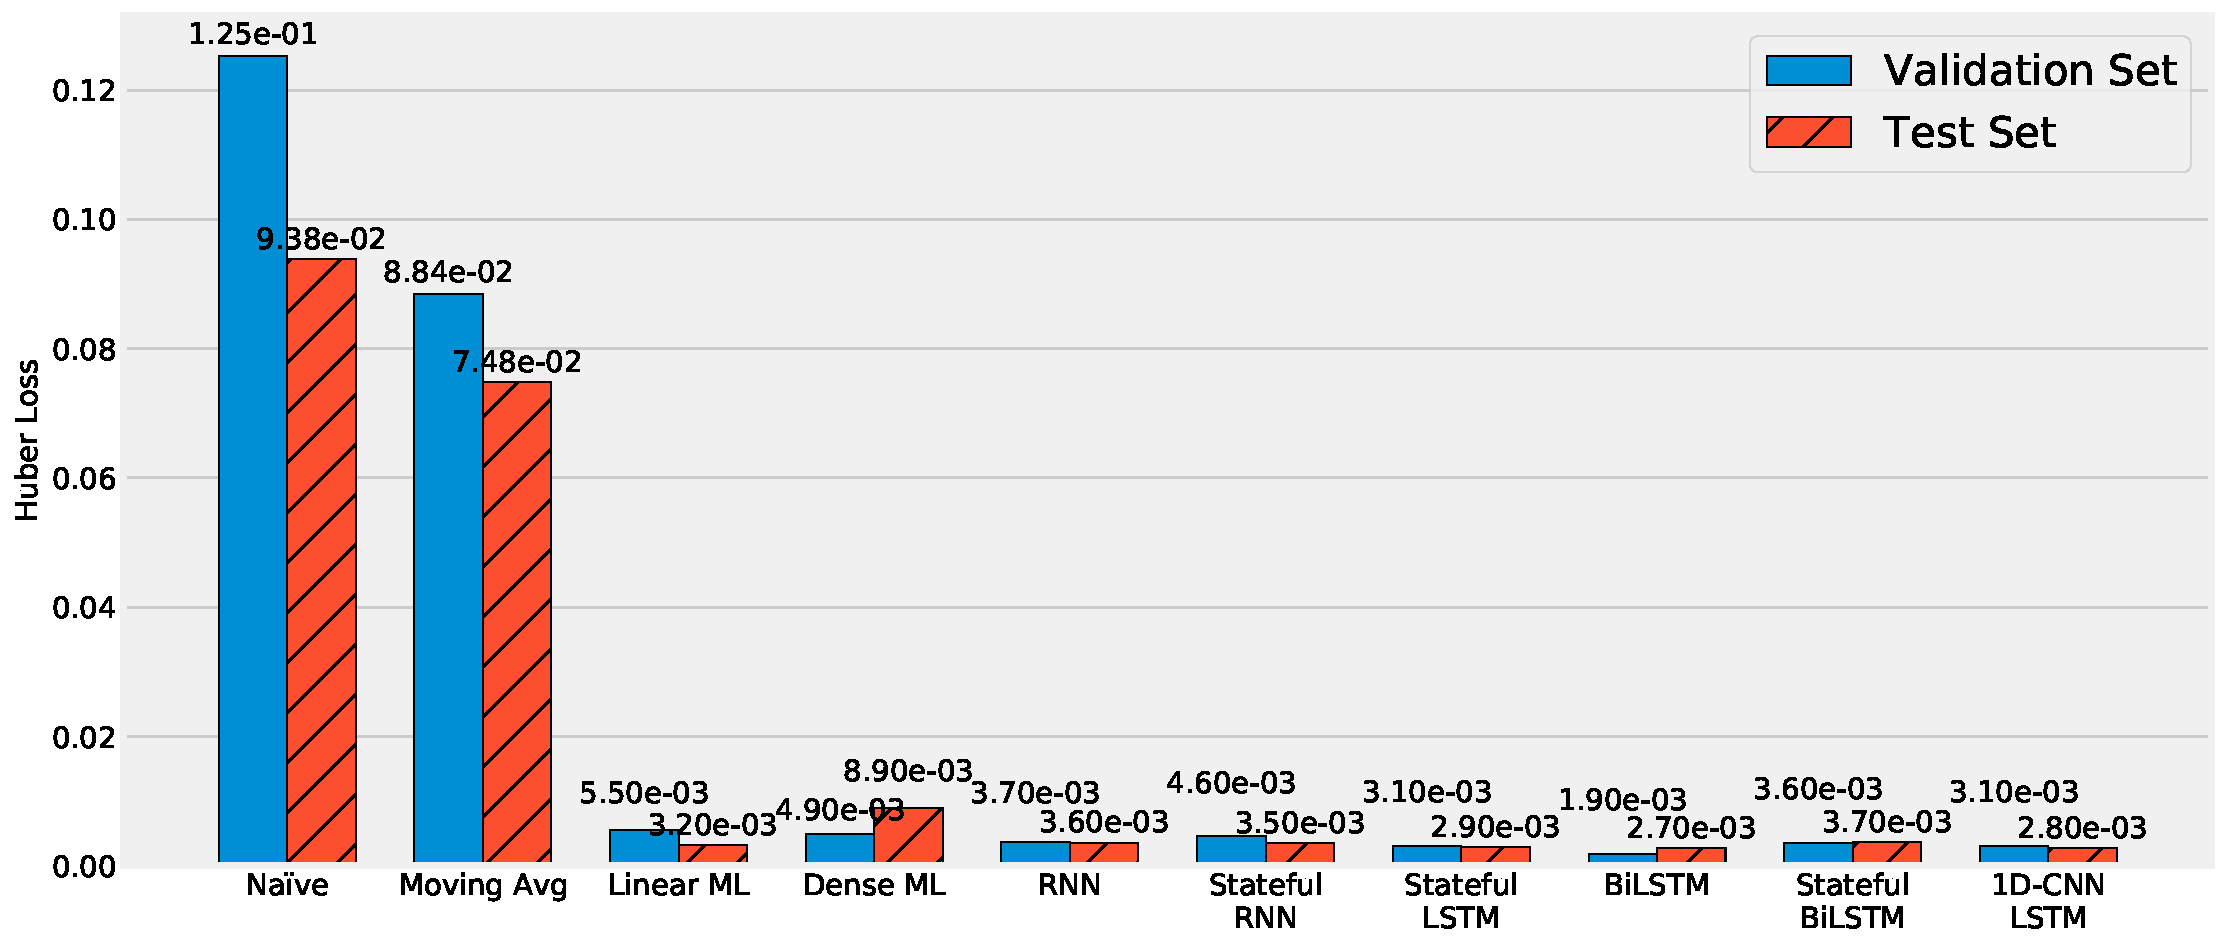
\includegraphics[width=\textwidth]{chapter4/figs/models_benchmark.pdf}}
    \caption{Benchmarking of 10 models, shows the Huber loss for the validation and test sets.}
\label{fig_benchmark}
\end{figure}

After experiments with different loss functions and evaluate their performance on our dataset, we chose the Huber function~\ref{eq_huber} as the loss function and the Mean Absolute Error (MAE) is used as the metric function to monitor the model performance.
We used the Huber function because it is robust and combines the advantages of both Mean Squared Error (MSE) and MAE loss functions. It is less sensitive to outliers than MSE, while still being differentiable and providing gradients, unlike MAE. Since our data is noisy and contains outliers that may negatively impact the model's performance, the Huber loss function is a good choice.

We examined various neural network models to determine the optimal architecture for our task.
Initially, we started with a simple linear model comprising of a single layer with a single neuron. However, this model did not yield satisfactory results.
We then explored a dense ML model consisting of two hidden layers, each with 32 neurons and a \textit{RelU} activation function. Next, we experimented with a simple RNN model with the same number of hidden layers and neurons.
To find the optimal learning rate, we utilized the \textit{LearningRateScheduler} callback function and discovered that a rate of 1.58e$^{-4}$ under the basic settings minimized the loss.
We proceeded to examine stateful versions of RNN, LSTM, and BiLSTM models with three hidden layers, each with 32 neurons and a learning rate of 1.58e$^{-4}$.
In addition, we explored a hybrid model that consisted of a 1-dimensional convolutional layer with 32 filters, a kernel size of 5, and a \textit{RelU} activation function. We combined this with a two-hidden layer LSTM network with 32 neurons each and a learning rate of 1.58e$^{-4}$. We experimented with \textit{Dropout} layers but did not observe any significant improvement in the results.
Finally, we evaluated a BiLSTM model with five hidden layers, 64 neurons each, and a learning rate of 0.001.
Based on the evaluation of all the models on both the validation and test sets (Fig.~\ref{fig_benchmark} and Table~\ref{table_models_config}), we selected the BiLSTM model for further refinement. More details on the final model architecture and hyperparameters are explained in the Appendix~\ref{config_appendix}.
Figure~\ref{fig_benchmark} presents a comparative analysis of the Huber loss within the validation and testing sets across the ten aforementioned models.
We used several evaluation measures to assess our models since each metric provides valuable insights into the accuracy and performance of the forecasts (Appendix~\ref{eval_appendix}), helping to identify areas for improvement and adjust the forecasting models accordingly.

\section{Results and discussion}
\label{sec_ch4_results}
The benchmarking in Figure~\ref{fig_benchmark} showed that, in general, the ML-based methods were not much different. On the other hand, the persistence model and moving average model resulted in the highest errors compared with the ML-based models, and their results were close to some extent. 
As we see, the BiLSTM model performed the best over both the validation and test sets compared with the other models.

We developed and trained 3 BiLSTM models to forecast the integral flux of SEP, one model per energy channels. After the training was completed, we evaluated the performance of the models from the loss curve (Fig.~\ref{fig_lossCurve}) using the Huber loss (the left panel) and the metric MAE (the middle panel). During the training, the learning rate was reduced multiple times via the \textit{LearningRateScheduler} callback function (the right panel).
The left panel quantifies the discrepancy between the model's predictions and the true values over time. It shows how the Huber loss function changes during the training iterations (Epochs) for the training and validation sets for the three energy channels so that each channel has one color.
The middle panel shows how the model's metric MAE changes with training epochs. It is used to evaluate the performance of the trained model by measuring the average absolute difference between the model's predictions and the true values, providing a single numerical value that indicates the model's error at a given epoch.
The right panel shows how the learning rate of the model's optimizer changes with epochs via the \textit{LearningRateScheduler} callback function, which changes the learning rate based on a predefined schedule to improve training efficiency and convergence.
The learning rate refers to the rate at which the model's parameters are updated during the training process.
We noticed that at the epochs where the learning rate has changed, there were bumps in the loss curves across all the energy channels, which is expected. This highlights the boundaries within which the learning rate yields better performance.

\begin{figure}[htp]
    \centerline{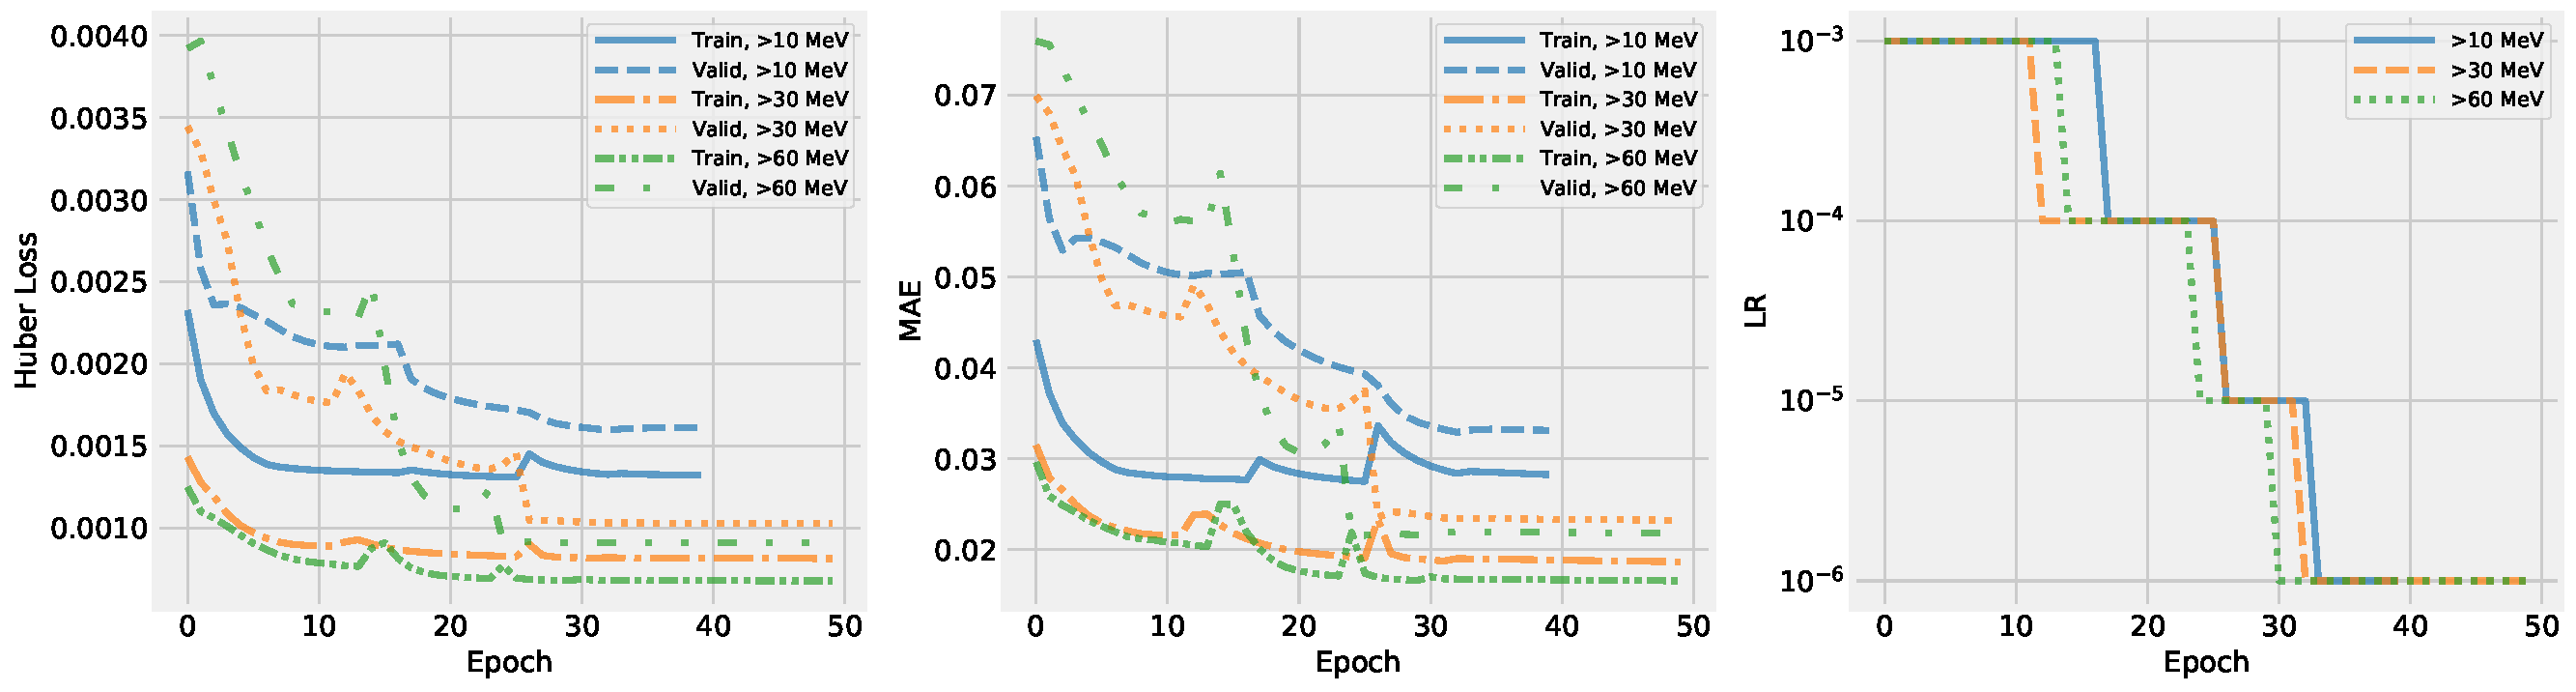
\includegraphics[width=\textwidth]{chapter4/figs/loss_curve_allenergies.pdf}}
    \caption{\textit{Left Panel} - The Huber loss vs. the number of training epochs for the BiLSTM model for the validation and test sets, for the 3 energy channels. \textit{Middle Panel} - The mean absolute error (MAE); the model's metric vs. the number of training epochs. \textit{Right Panel} - Shows how the learning rate of the Adam optimizer changes over the number of epochs.}
\label{fig_lossCurve}
\end{figure}

From experimentation, we found that the batch size and the optimizer learning rate are the most important hyperparameters that have a strong influence on the overall model's performance \citep{greff_2016}.
In addition, adding \textit{dropout} layers as well as varying the number of hidden layers and hidden neurons resulted in only marginal improvements to the final model performance, while substantially increasing training time and requiring greater computational resources.

The term \textit{batch size} refers to the number of data sequences processed in one iteration during the training of a ML model \citep{goodfellow_2016}. Initially, a batch size of 64 was selected, however, we observed that the model produced better results when a batch size of 30 was used instead. This could be related to the Carrington rotation, which lasts for $\sim$27 days. There were $\sim$570 Carrington rotations between December 25$^{th}$ 1976 and July 30$^{th}$ 2019. Therefore, updating the model's weights after every Carrington rotation could be a reasonable choice for improving its performance.
Figure~\ref{fig_model_vs_obs_valset} shows how good the model predictions are (on the y-axis) compared with the observations of the validation set (on the x-axis). The blue, orange, and gold colors refer to 1-day, 2-day, and 3-day ahead predictions, respectively. The top panel is for the $>$10 MeV channel, the middle panel is for the $>$30 MeV channel, and the bottom panel is for the $>$60 MeV channel. The left column is for the entire validation set, while the right column is for the observations points $\geq$10 proton flux units (pfu). That is the threshold value of proton flux as measured by the National Oceanic and Atmospheric Administration (NOAA) GOES spacecraft to indicate severity of space weather events caused by SEP.

\begin{figure}[htp]
    \centering
    \begin{subfigure}
         \centering
         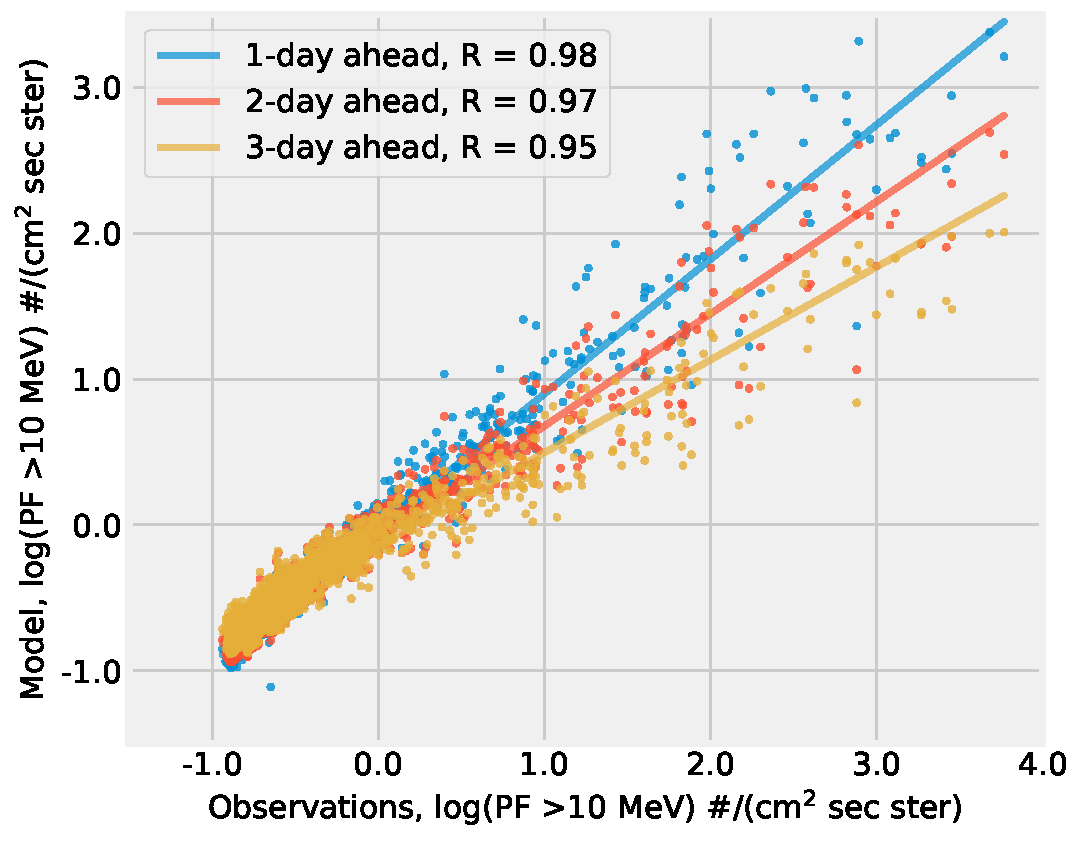
\includegraphics[width=0.4\textwidth]{chapter4/figs/scatterplot_obs_vs_model_valset_3in1_log_PF10.pdf}
    \end{subfigure}
    %\hfill
    \begin{subfigure}
         \centering
         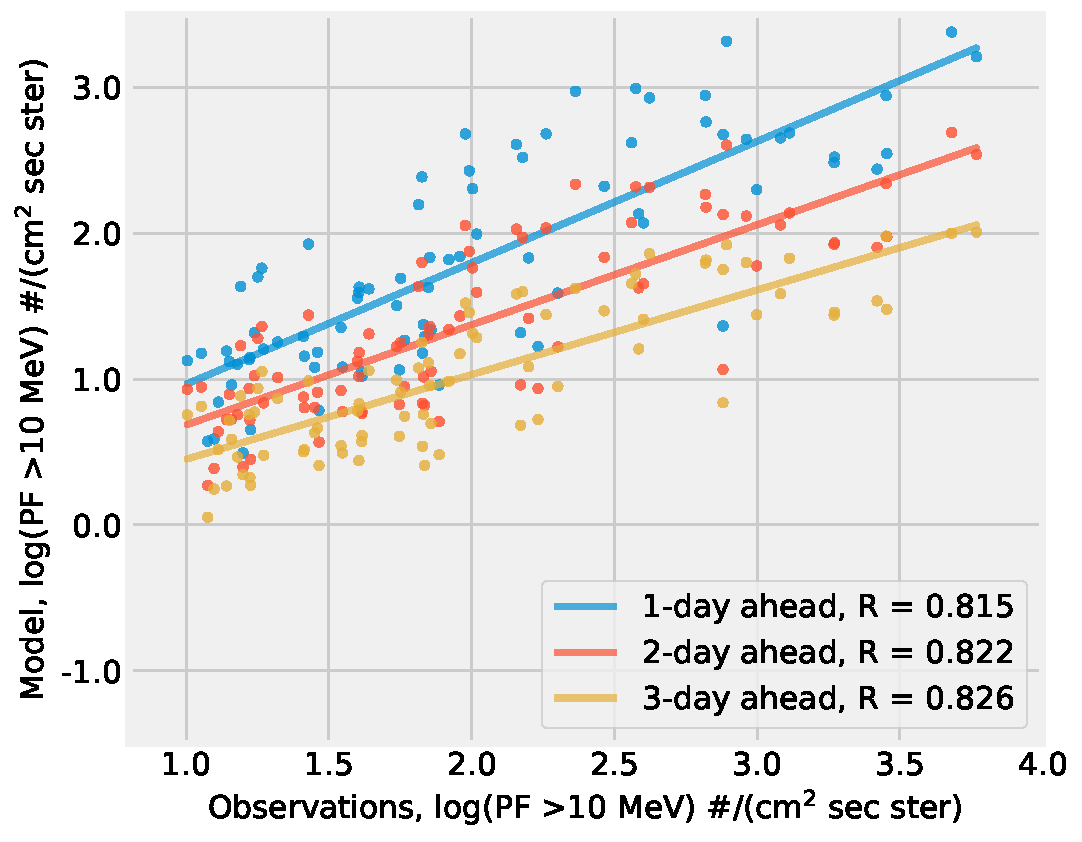
\includegraphics[width=0.4\textwidth]{chapter4/figs/scatterplot_obs_vs_model_valset_3in1_LOG_PF_LT1_log_PF10.pdf}
    \end{subfigure}
    \begin{subfigure}
         \centering
         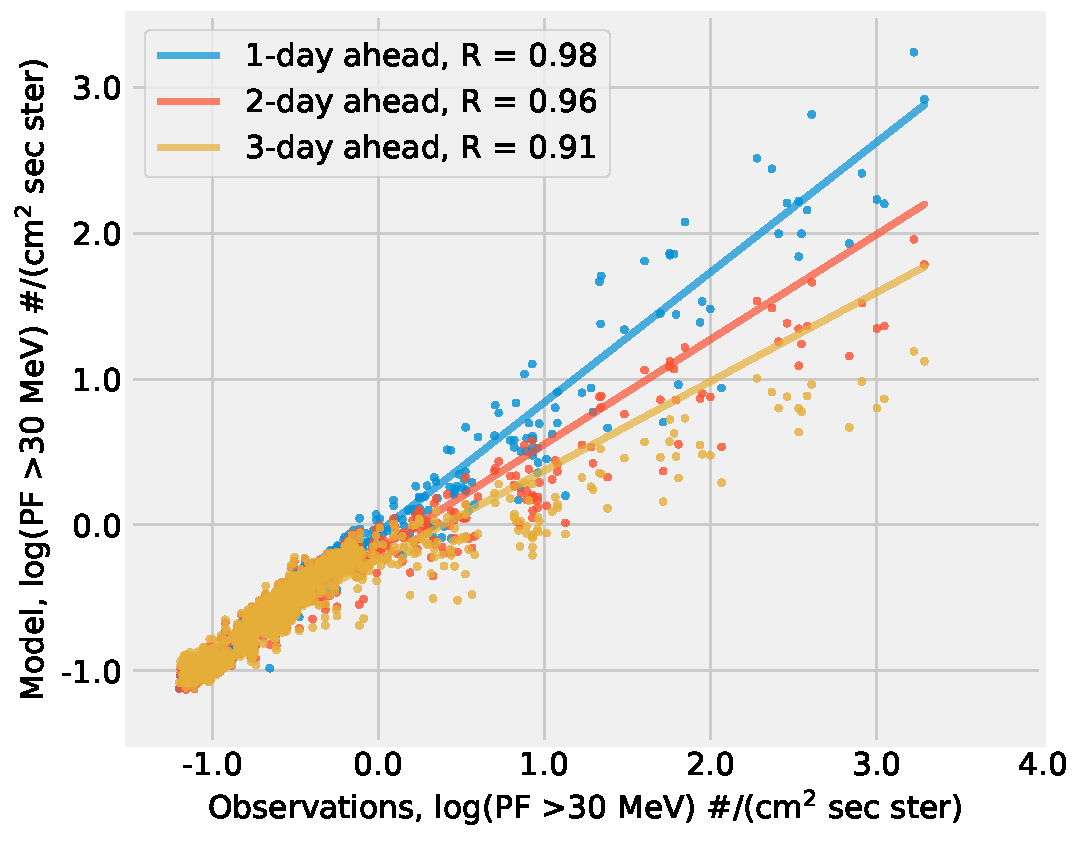
\includegraphics[width=0.4\textwidth]{chapter4/figs/scatterplot_obs_vs_model_valset_3in1_log_PF30.pdf}
    \end{subfigure}
    %\hfill
    \begin{subfigure}
         \centering
         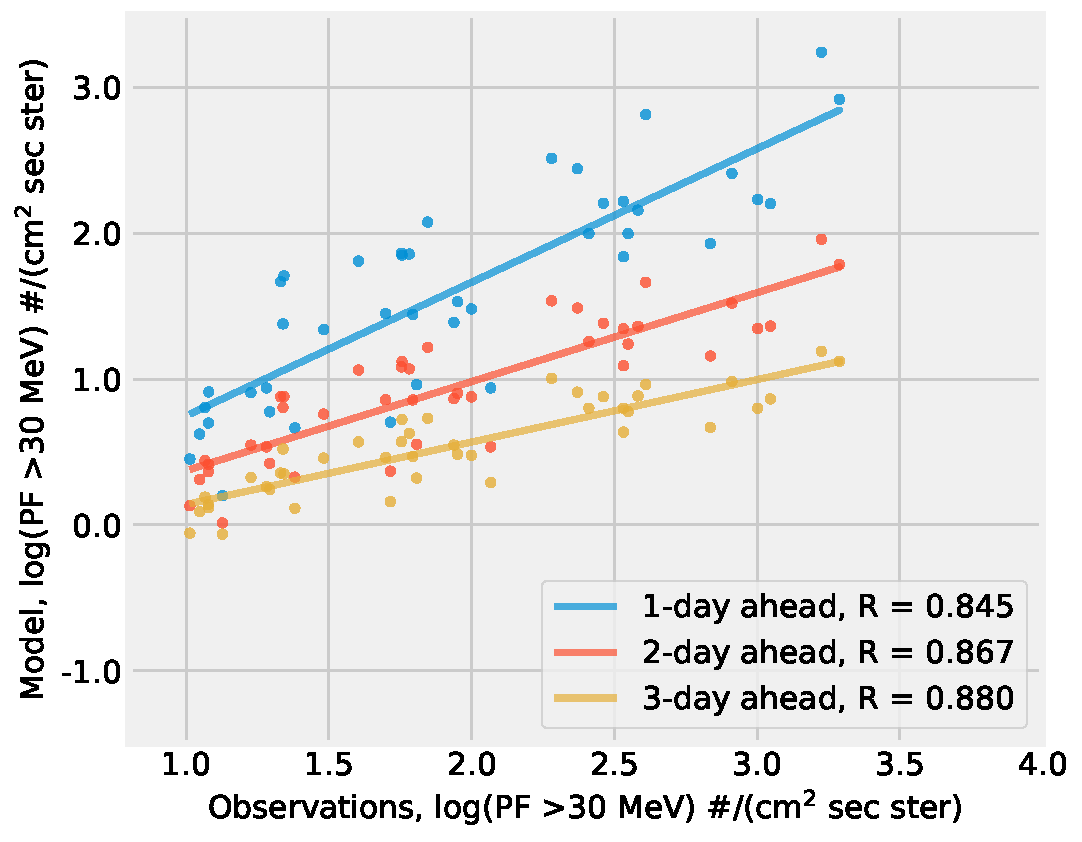
\includegraphics[width=0.4\textwidth]{chapter4/figs/scatterplot_obs_vs_model_valset_3in1_LOG_PF_LT1_log_PF30.pdf}
    \end{subfigure}
    \begin{subfigure}
         \centering
         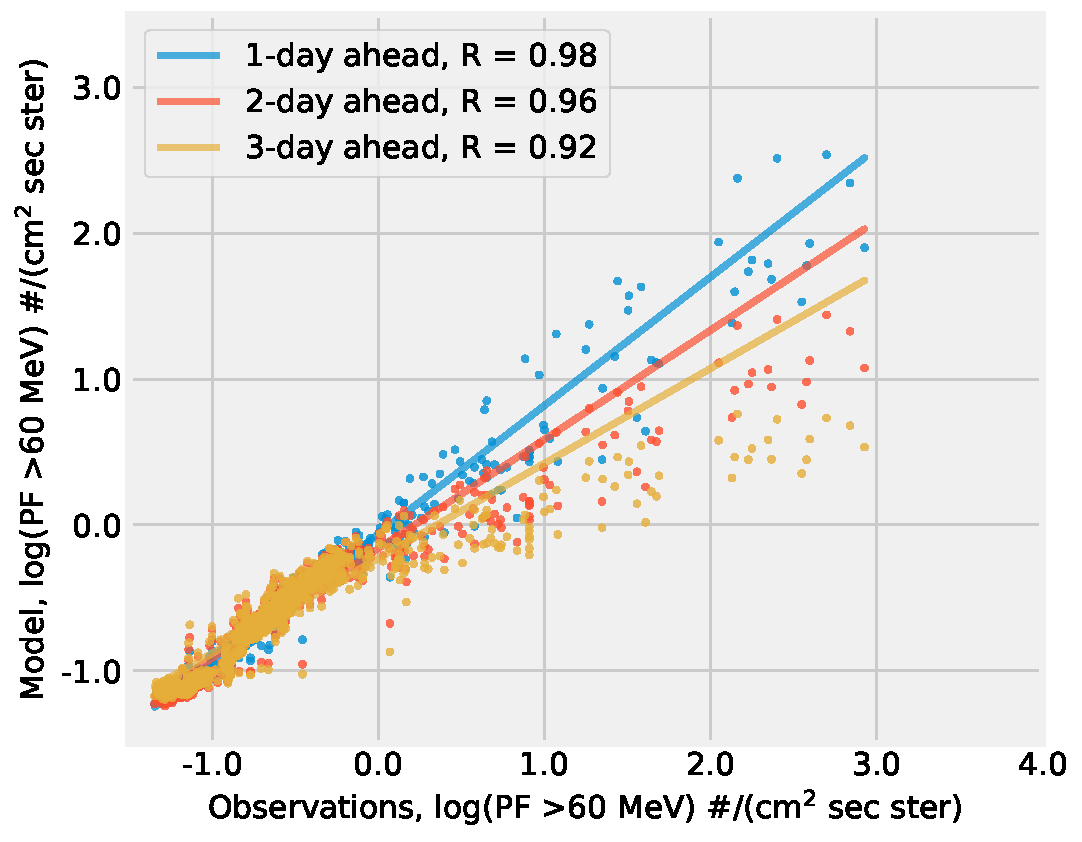
\includegraphics[width=0.4\textwidth]{chapter4/figs/scatterplot_obs_vs_model_valset_3in1_log_PF60.pdf}
    \end{subfigure}
    %\hfill
    \begin{subfigure}
         \centering
         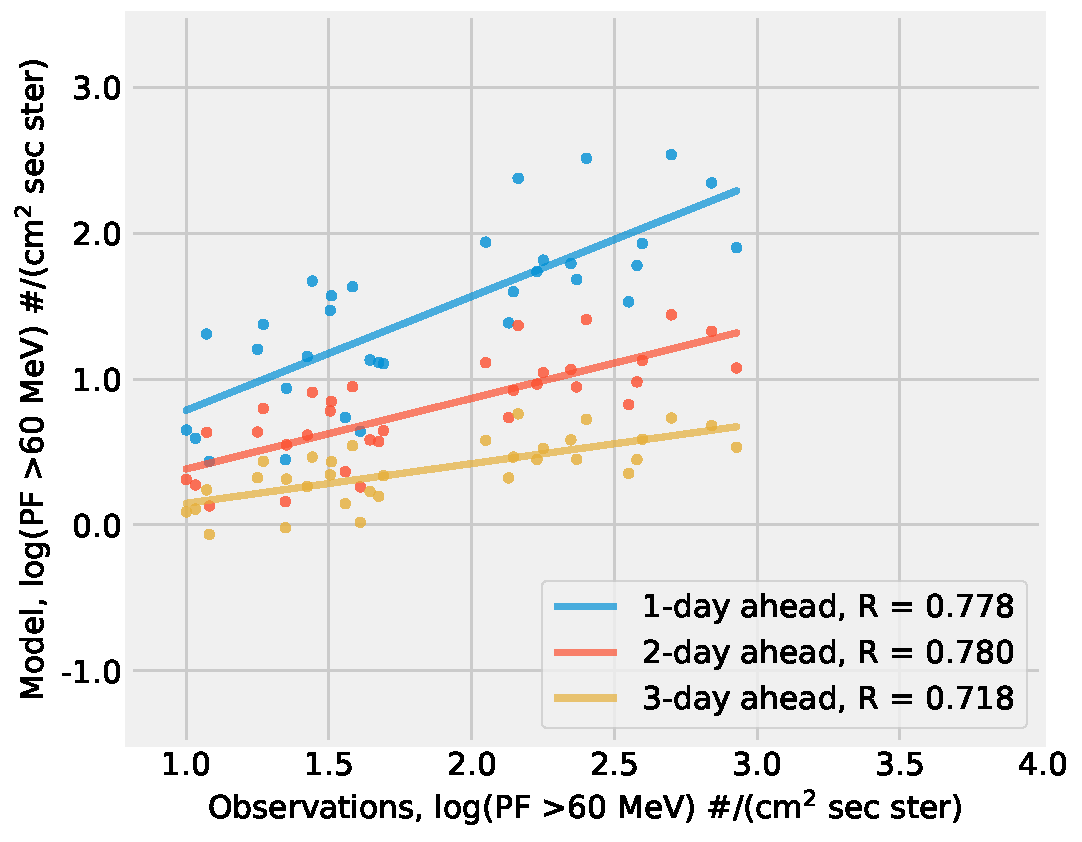
\includegraphics[width=0.4\textwidth]{chapter4/figs/scatterplot_obs_vs_model_valset_3in1_LOG_PF_LT1_log_PF60.pdf}
    \end{subfigure}
\caption{Correlation between the model predictions and observations for 1-day, 2-day, and 3-day ahead for $>$10 MeV (top panel), $>$30 MeV (middle panel), and $>$60 MeV (bottom panel). The panels in the left column represent all the points of the validation set, those in the right column represent all the observations points with daily mean flux $\geq$10 pfu.}
\label{fig_model_vs_obs_valset}
\end{figure}

We found that, overall, the models performed very well. The $R$ correlation was $>$0.9 for all points of the validation set across the forecasting windows for the 3 energy channels. The $R$ correlation was $>$0.7 for the observations points $\geq$10 pfu as well. However, the correlation between the modeled data and the observations exhibited a decline as the forecast horizon increased, in accordance with the anticipated result.
To confirm the validity of the models, we performed the same correlation analysis between the modeled data and the observations of the out-of-sample test set (Fig.~\ref{fig_model_vs_obs_tstset}), which was not given to the model. Again, we found a high correlation across the forecasting windows for the 3 energy channels. 
The points were more dispersed between 1 and 1.5 on the x-axis, which reflected in a bit lower correlation. This might be a limitation in the current version of the model between that range of SEP fluxes since the models underestimated the flux values within that range across all energy channels, possibly due to the relatively smaller training samples with fluxes above 10 pfu compared with the majority of the data.

\begin{figure}[htp]
    \centering
    \begin{subfigure}
         \centering
         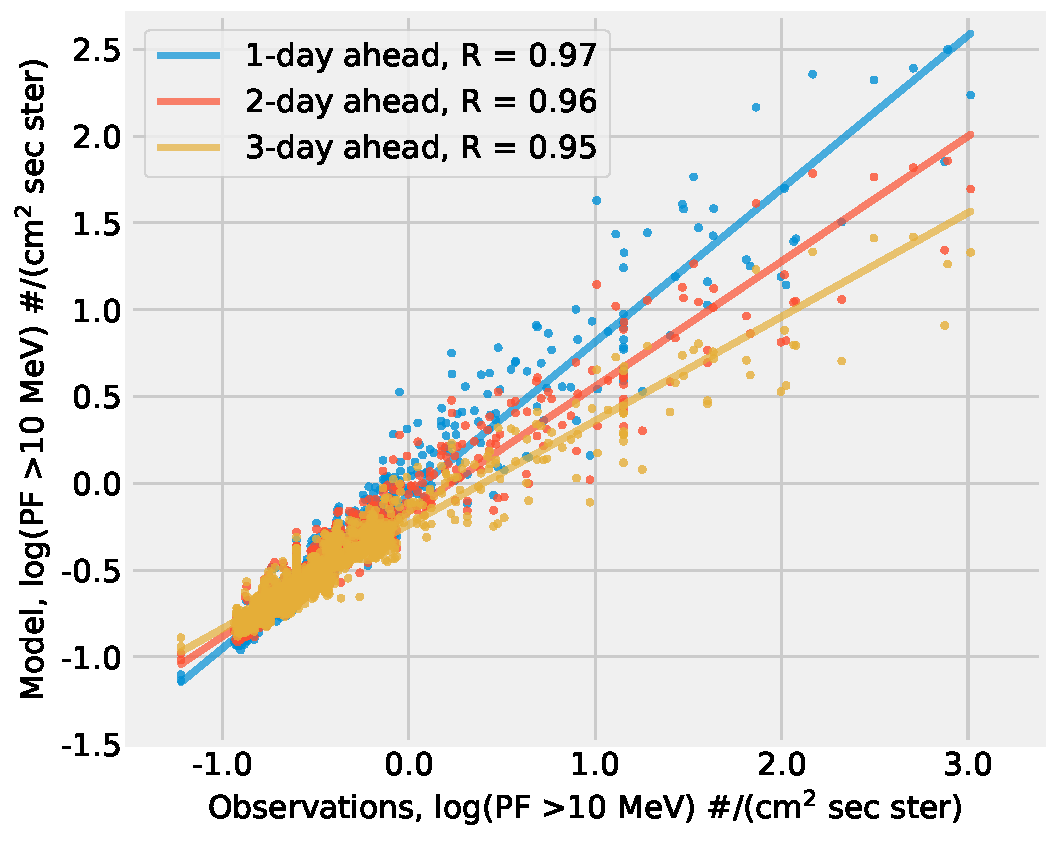
\includegraphics[width=0.4\textwidth]{chapter4/figs/scatterplot_obs_vs_model_tstset_3in1_log_PF10.pdf}
    \end{subfigure}
    %\hfill
    \begin{subfigure}
         \centering
         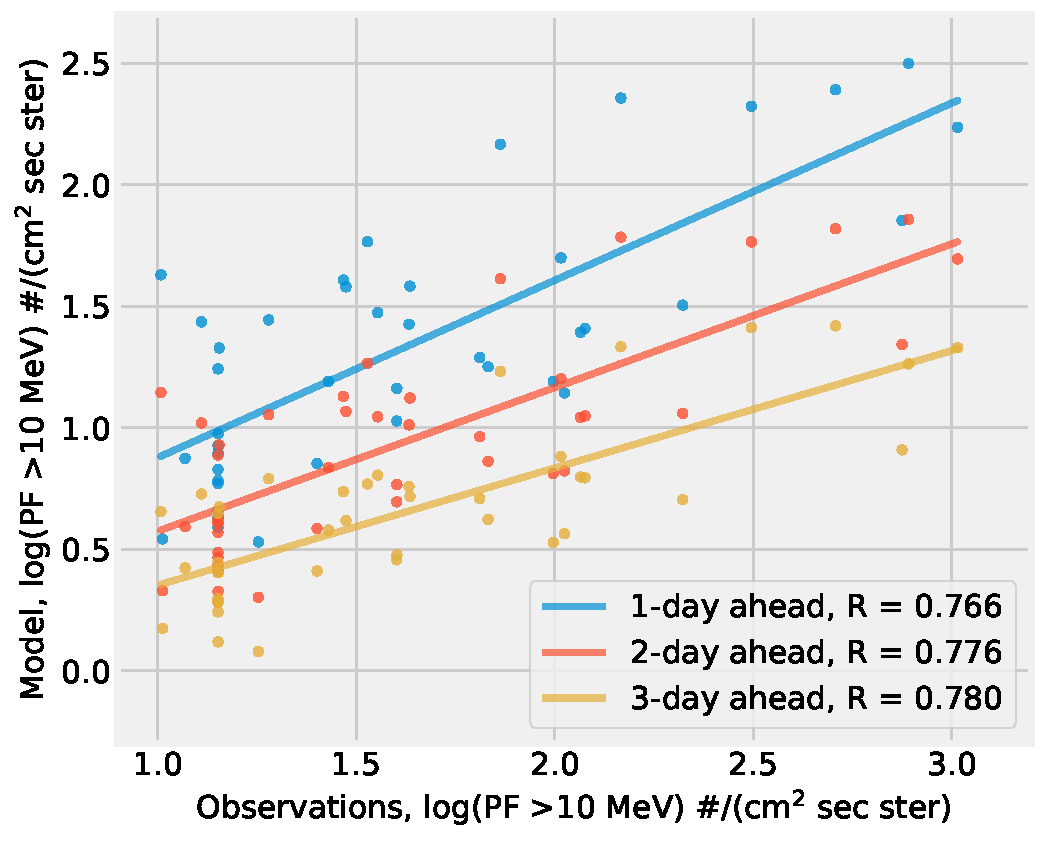
\includegraphics[width=0.4\textwidth]{chapter4/figs/scatterplot_obs_vs_model_tstset_3in1_LOG_PF_LT1_log_PF10.pdf}
    \end{subfigure}
    \begin{subfigure}
         \centering
         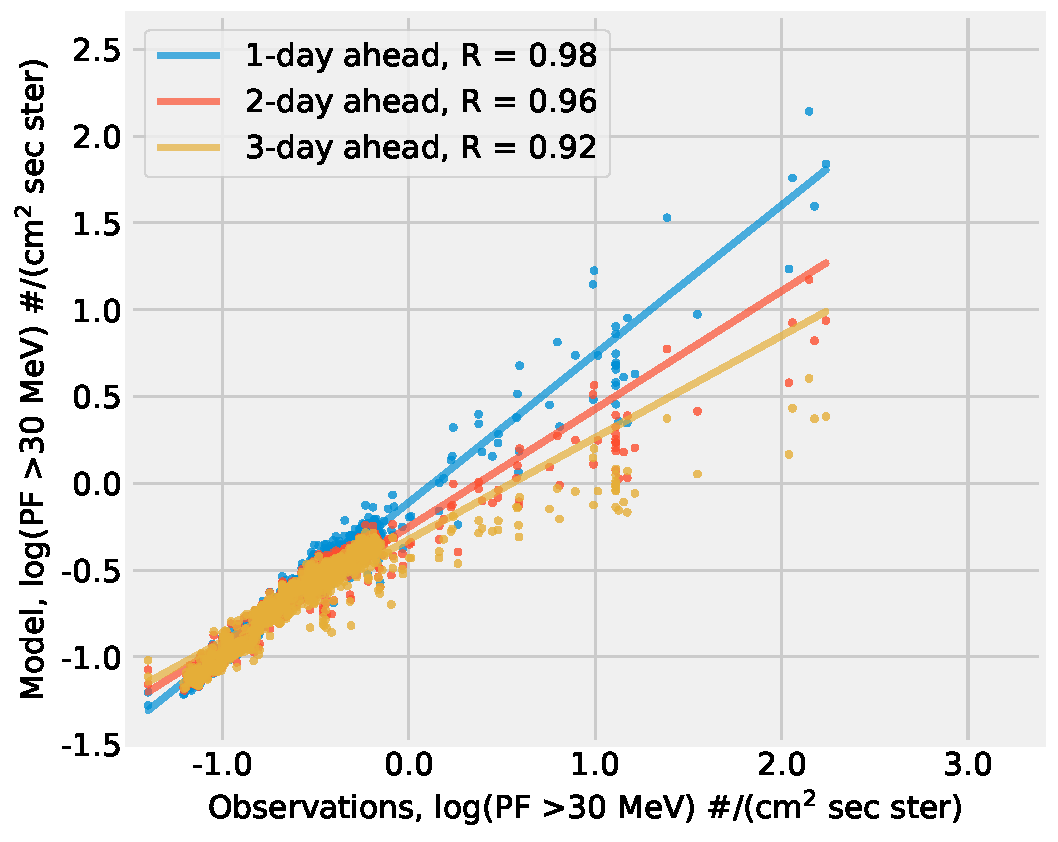
\includegraphics[width=0.4\textwidth]{chapter4/figs/scatterplot_obs_vs_model_tstset_3in1_log_PF30.pdf}
    \end{subfigure}
    %\hfill
    \begin{subfigure}
         \centering
         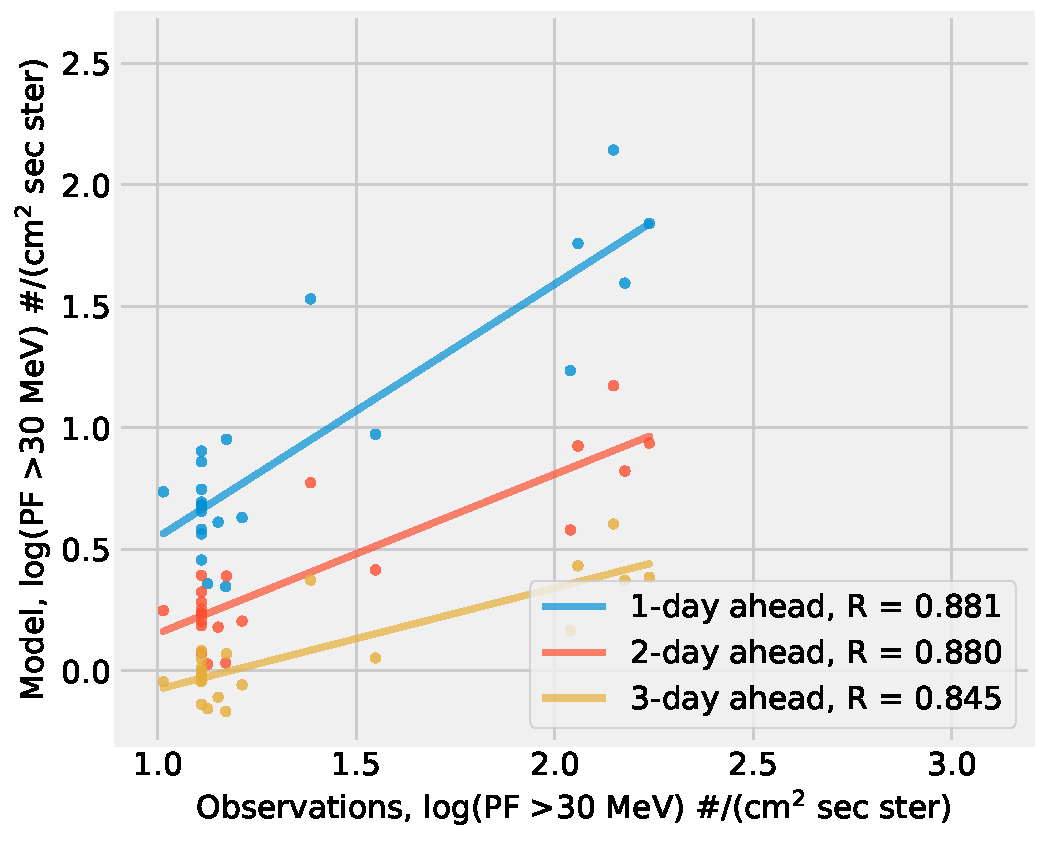
\includegraphics[width=0.4\textwidth]{chapter4/figs/scatterplot_obs_vs_model_tstset_3in1_LOG_PF_LT1_log_PF30.pdf}
    \end{subfigure}
    \begin{subfigure}
         \centering
         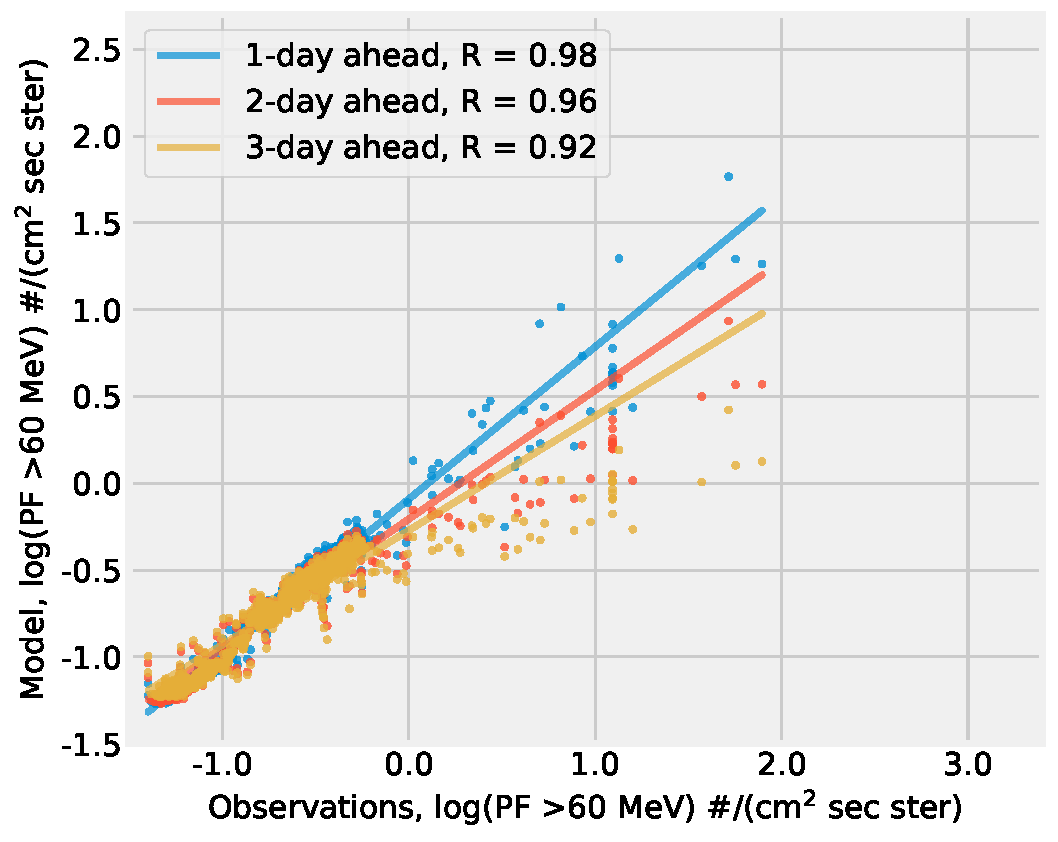
\includegraphics[width=0.4\textwidth]{chapter4/figs/scatterplot_obs_vs_model_tstset_3in1_log_PF60.pdf}
    \end{subfigure}
    %\hfill
    \begin{subfigure}
         \centering
         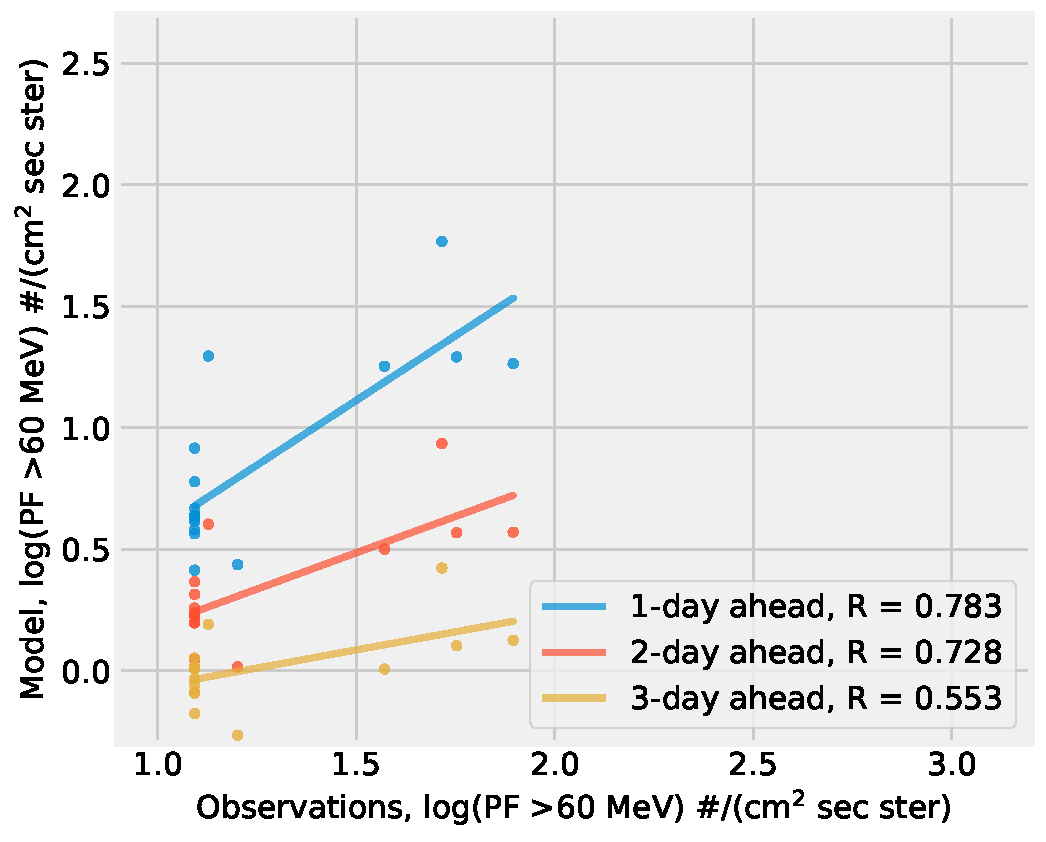
\includegraphics[width=0.4\textwidth]{chapter4/figs/scatterplot_obs_vs_model_tstset_3in1_LOG_PF_LT1_log_PF60.pdf}
    \end{subfigure}
\caption{Same as Figure~\ref{fig_model_vs_obs_valset} but for the test set.}
\label{fig_model_vs_obs_tstset}
\end{figure}

In order to see the temporal variation of the correlation between the modeled data and the observations, we applied a rolling window of 90 steps (3 months × 30 days/month = 1 season) that shows the seasonal variation of the correlation, as shown in Figure~\ref{fig_crosscorr_tstset}.  
Here, we show only the 1-day ahead predictions for the test set, for the 3 energy channels. 
We observe drops in the correlation factor synchronized with the transition between solar cycles (e.g., particularly between $\sim$1995 - 2000, which represents the declining phase of the solar cycle 22 and the rising phase of the solar cycle 23). This could be related to the fact that the low SEP fluxes during quiet times are more random and thus more difficult to forecast \citep{feynman_1990, gabriel_1990, rodriguez_2010, xapsos_2012}.

During periods of low solar activity, the forecasting of low SEP fluxes becomes more challenging due to their increased randomness. This difficulty arises from the reduced occurrence of conventional SEP drivers, such as solar flares and CMEs. Studies have suggested that the most significant solar eruptions tend to happen shortly before or after the solar cycle reaches its maximum \citep{vsvestka_1995}. Additionally, sporadic increases in solar activity have been observed \citep{kane_2011}, which might contribute to the diminished correlations observed in our research.
There is clearly some factor that is influencing the correlation during certain periods where there are no or only weak SEP events. However, it is not obvious which physical phenomena are the cause rather than, for instance, some artifact of the data. Understanding the interplay between these factors and their influence on SEP fluxes during periods of reduced solar activity remains a critical area of research. It would be interesting to find what is reducing the correlations, thus more investigation is needed.

Overall, the modeled data was correlated the most with observations at $>$60 MeV, then the second rank was for the $>$10 MeV channel, and the third rank was for the $>$30 MeV channel. That could be related to the relatively larger extent of drops in correlation at the $>$30 MeV channel.
The decline in correlation at the $>$30 MeV channel is consistent with the findings of \citet{le_2017}.
A summary of the performance results of the models for both the validation set and test set is presented in Table~\ref{table_performance}.

\begin{figure}[h!]
    \centerline{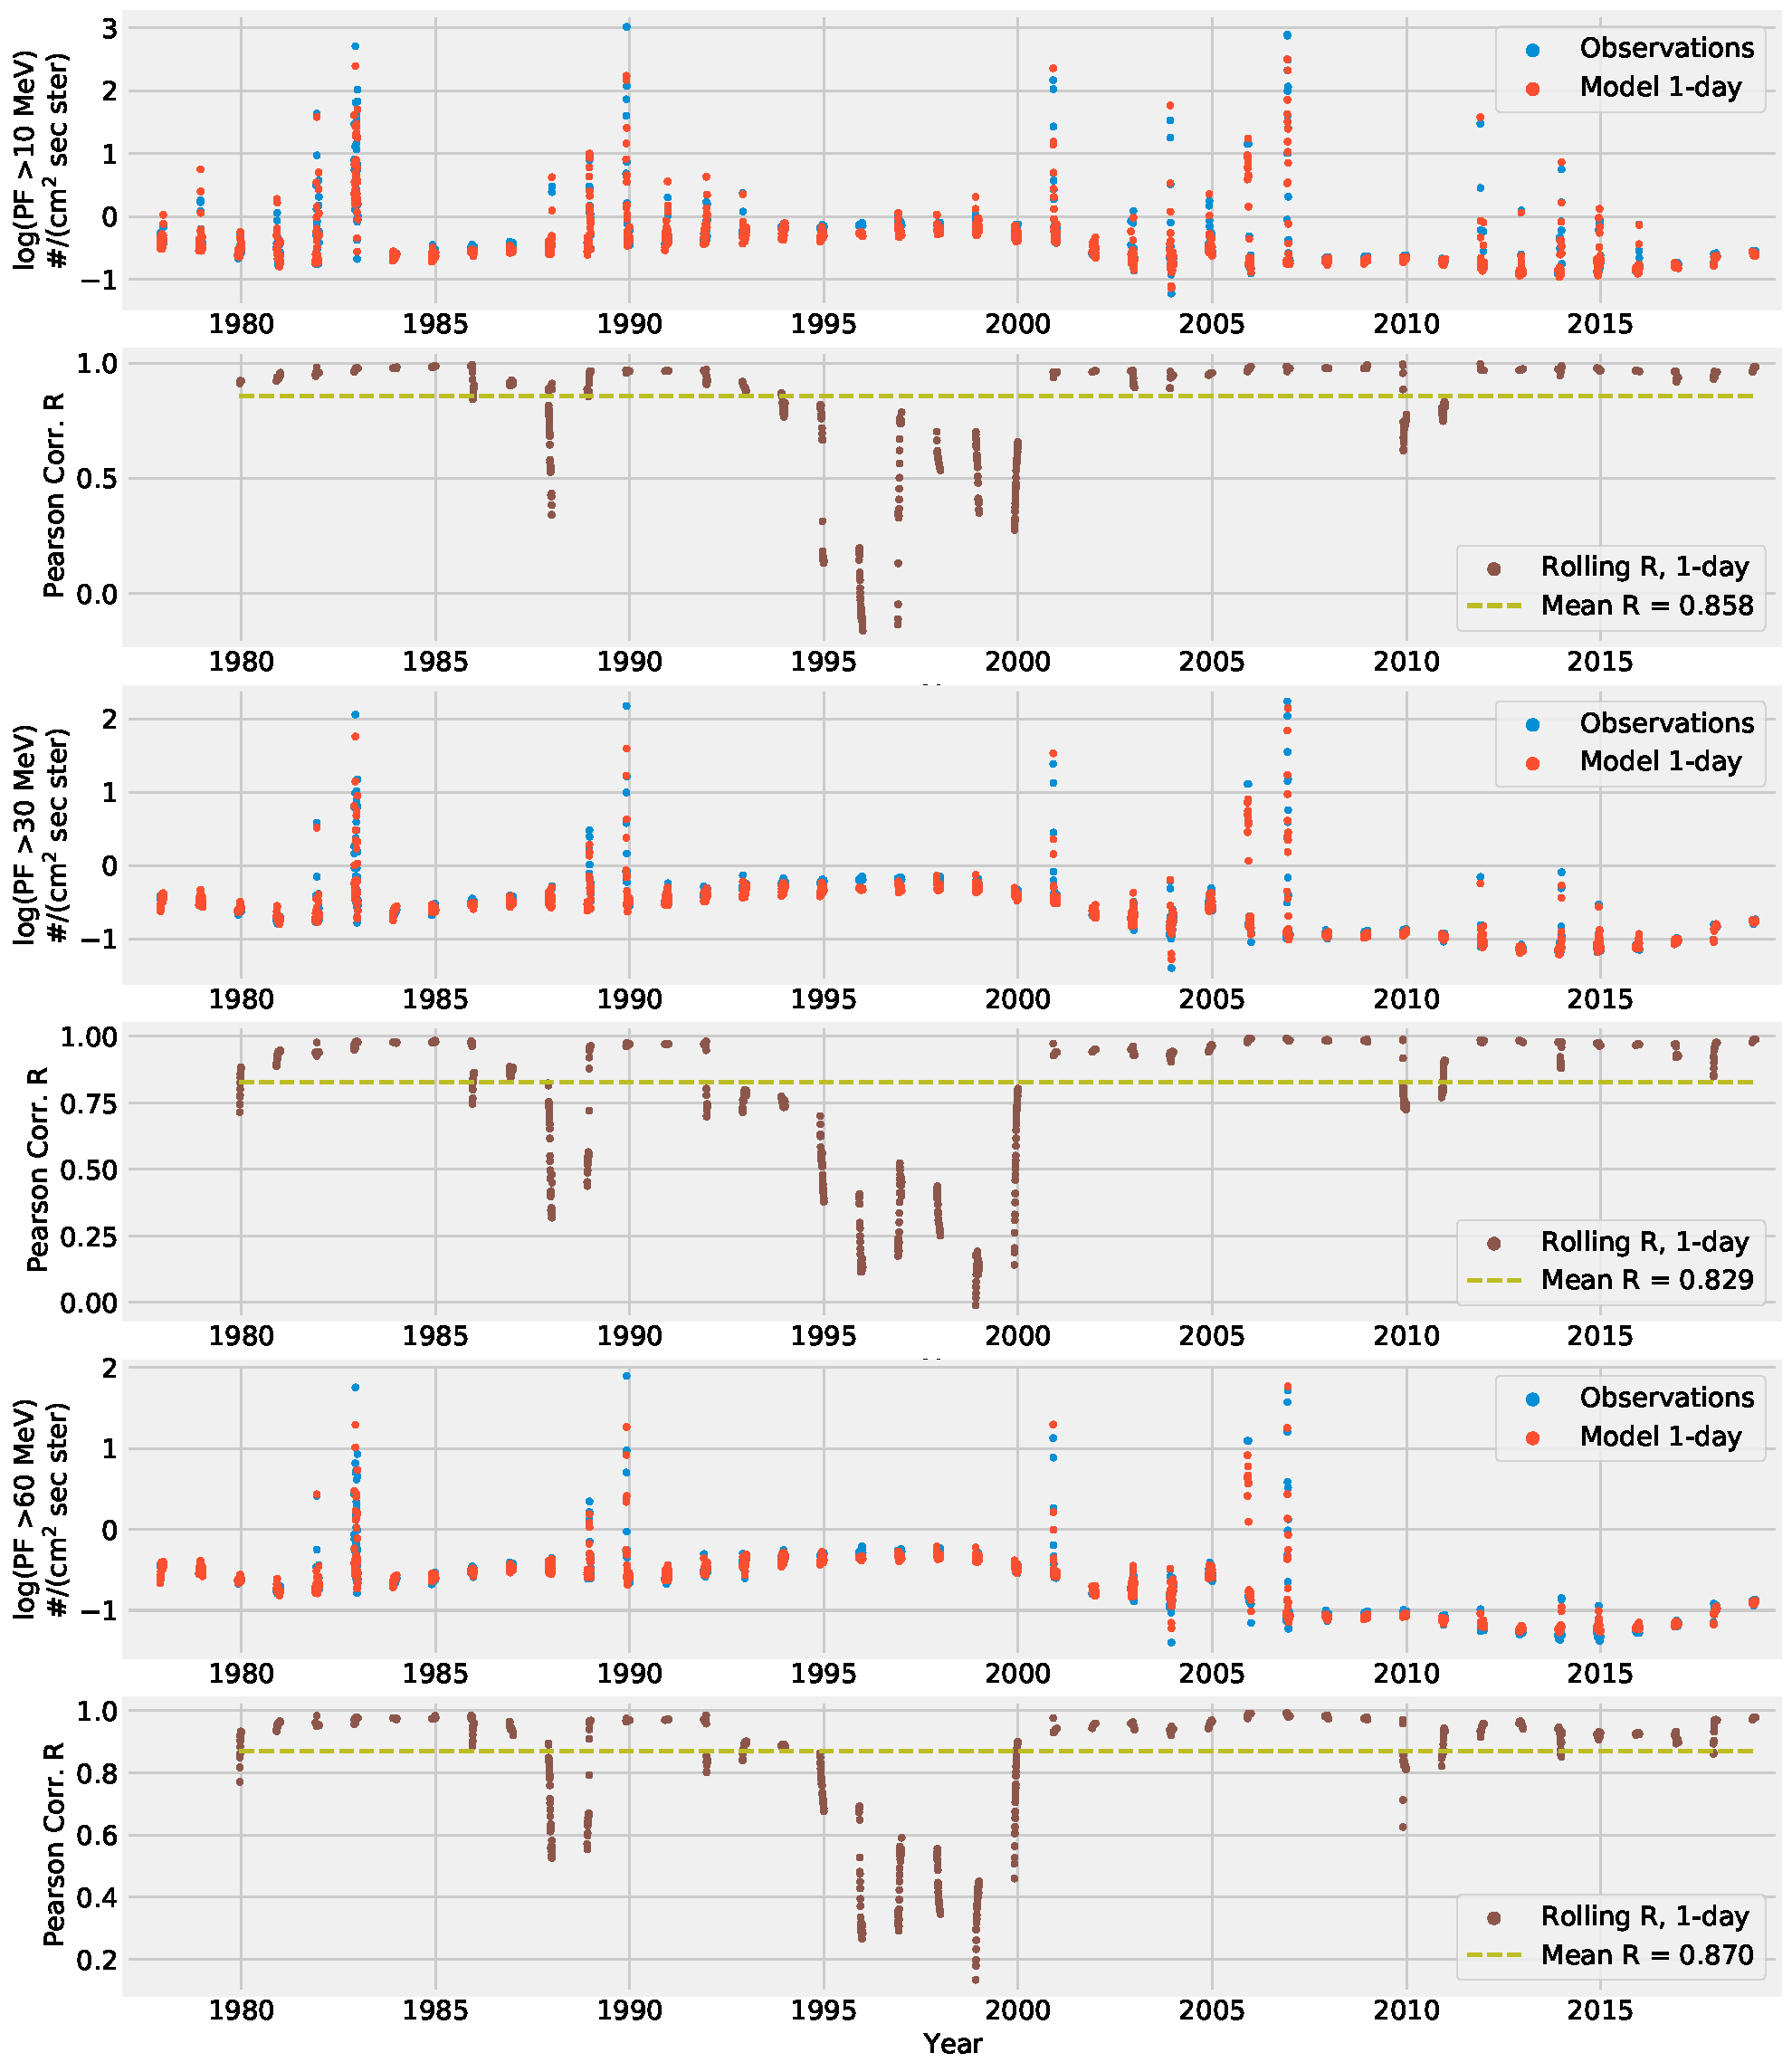
\includegraphics[width=\textwidth]{chapter4/figs/comparison_crosscorr_tstset_1day_3channels.pdf}}
    \caption{Comparison between the model outputs and observations of the test set for the 3 energy channels. In addition to the rolling-mean window correlation for 1-day ahead predictions.}
\label{fig_crosscorr_tstset}
\end{figure}

\begin{figure}[htp]
    \centerline{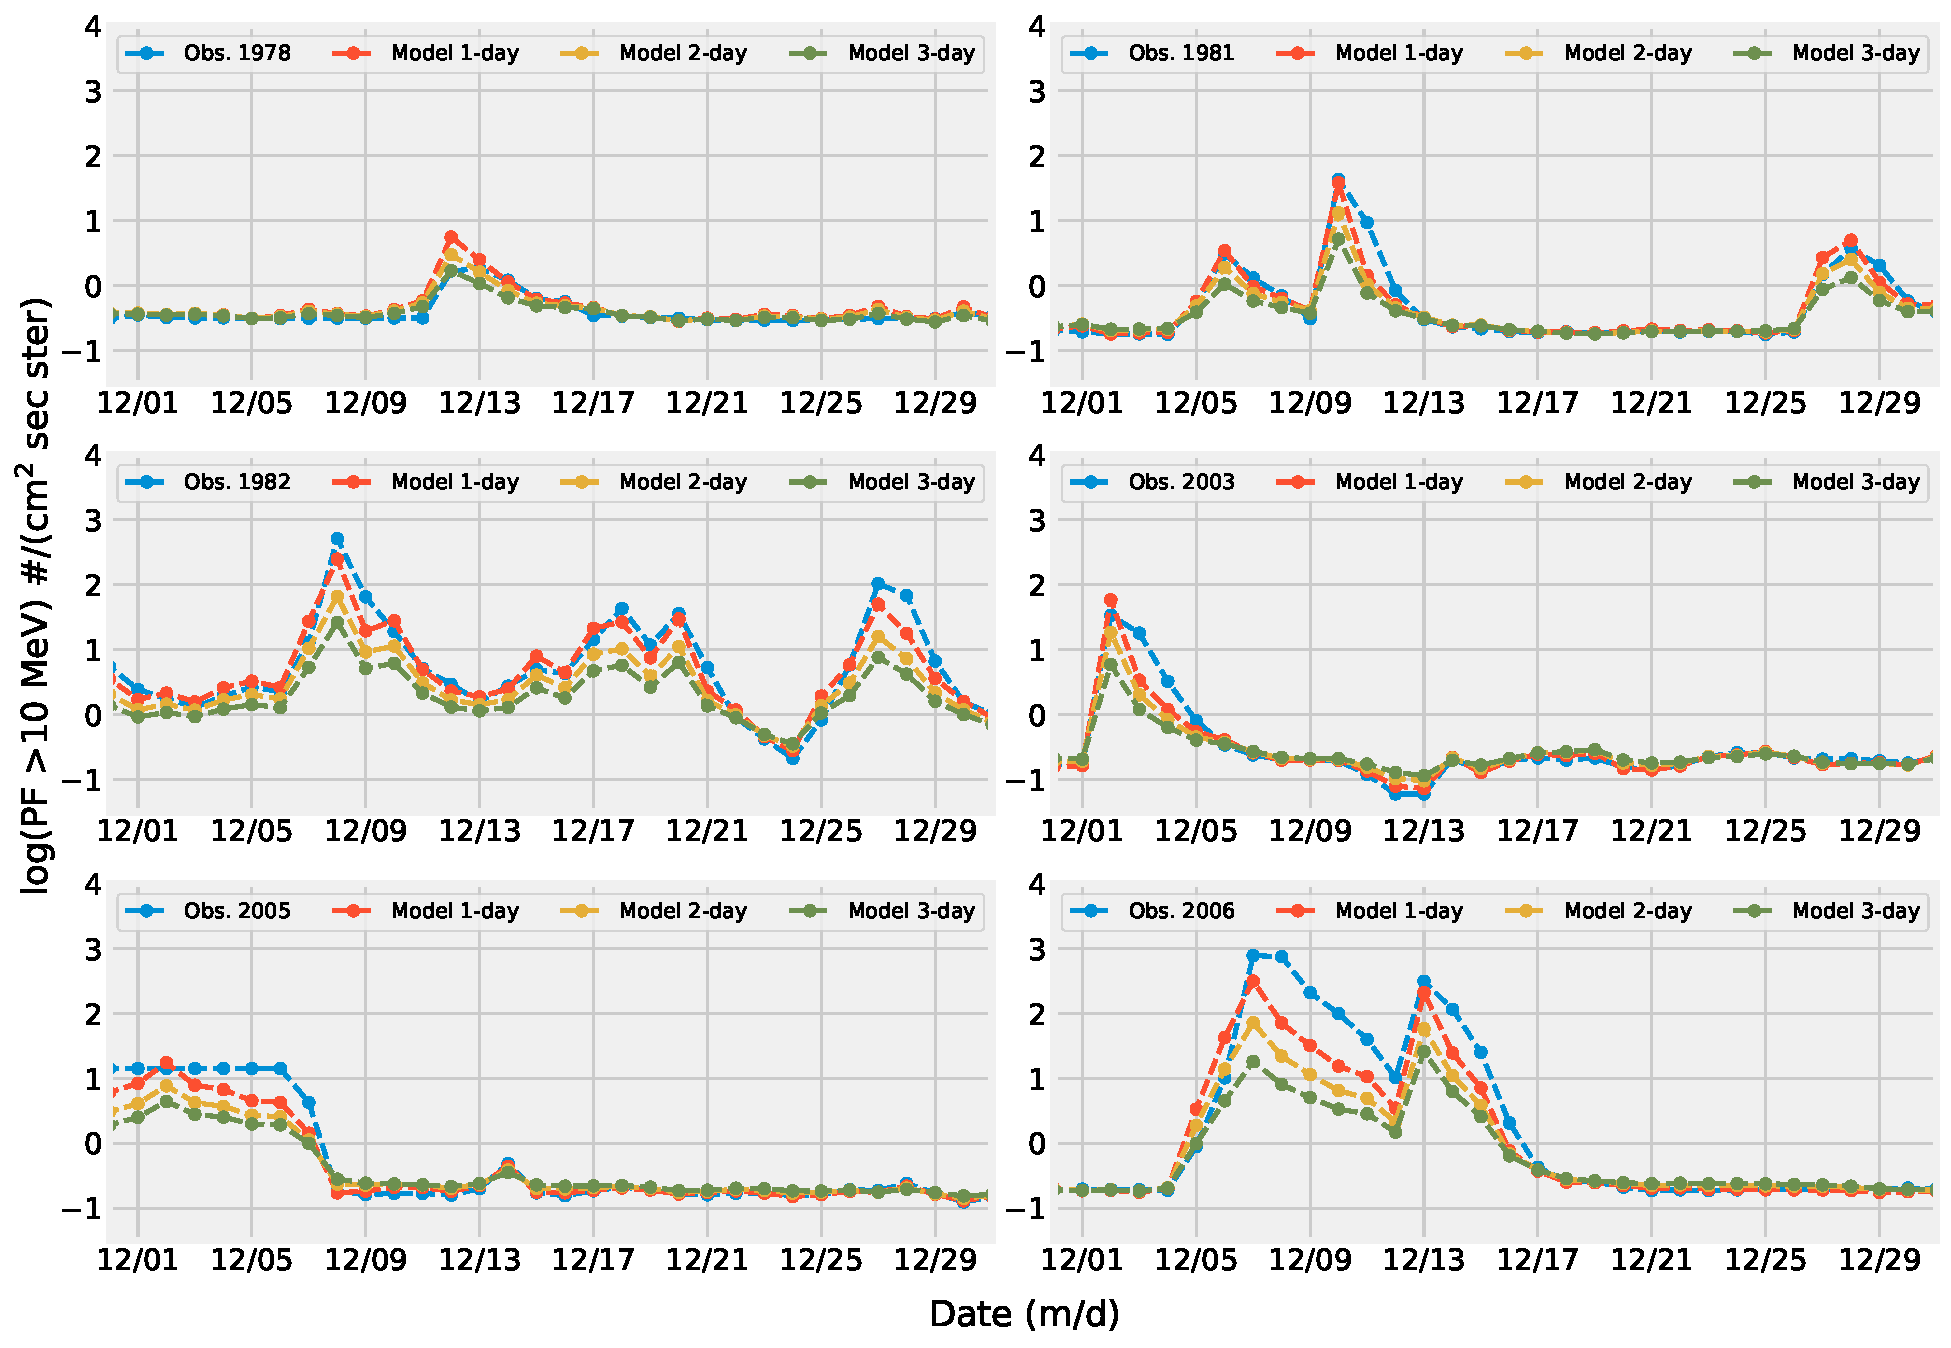
\includegraphics[width=\textwidth]{chapter4/figs/log_pf10/examples_10_tstset.pdf}}
    \caption{The model's forecasts for the out-of-sample testing set for the $>$10 MeV channel are shown at forecast horizons of 1 day, 2 days, and 3 days ahead, using samples of data from December in selected years mentioned in the top-left side of the plots.}
\label{fig_examples_pf10_tstset}
\end{figure}

\begin{figure}[htp]
    \centerline{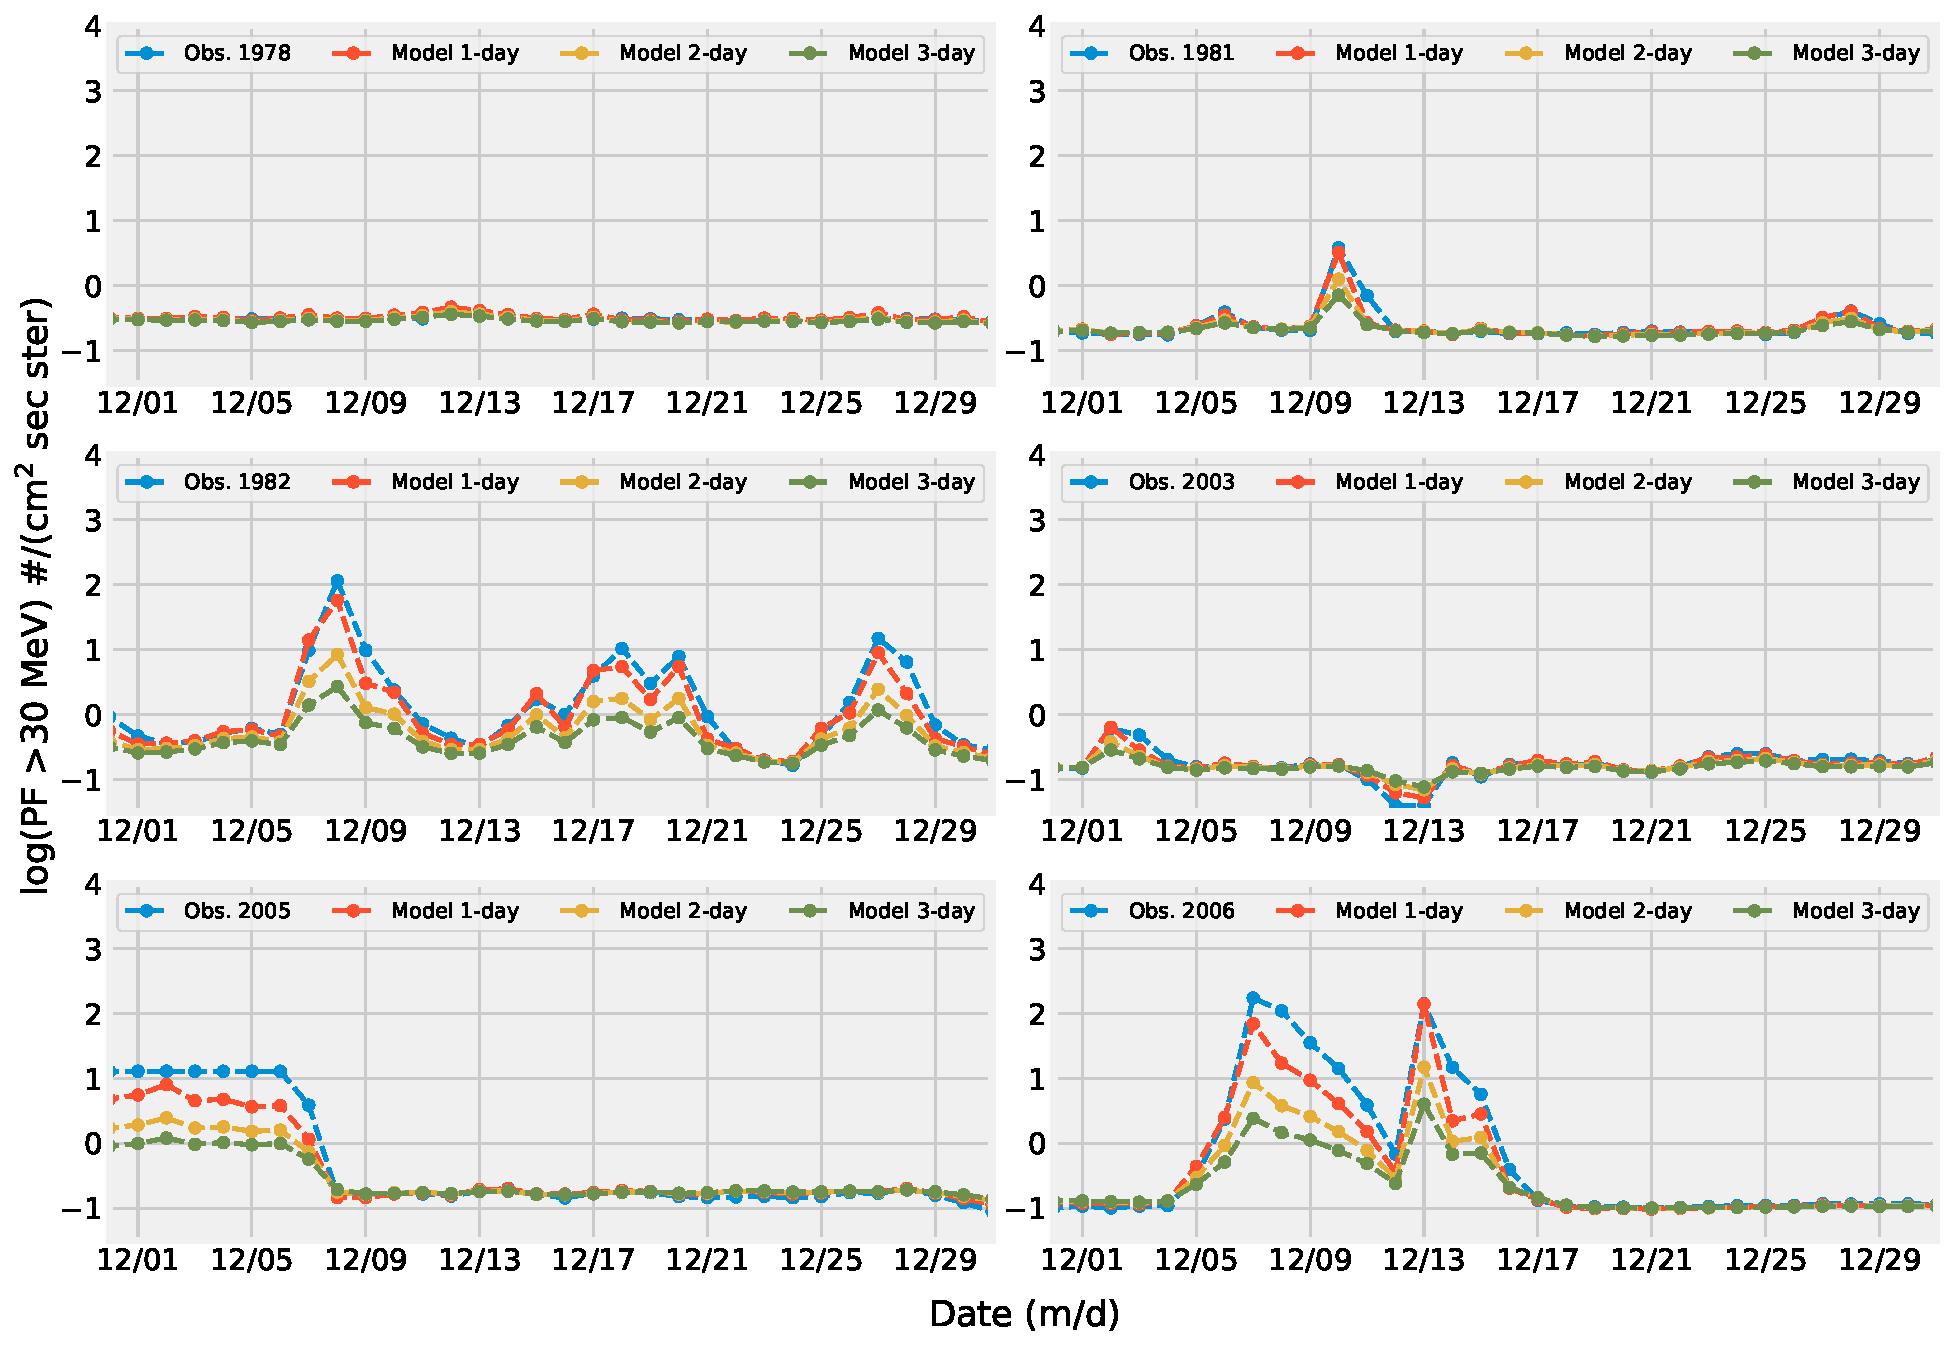
\includegraphics[width=\textwidth]{chapter4/figs/log_pf30/examples_30_tstset.pdf}}
    \caption{The model's forecasts for the out-of-sample testing set for the $>$30 MeV channel are shown at forecast horizons of 1 day, 2 days, and 3 days ahead, using samples of data from December in selected years mentioned in the top-left side of the plots.}
\label{fig_examples_pf30_tstset}
\end{figure}

\begin{figure}[htp]
    \centerline{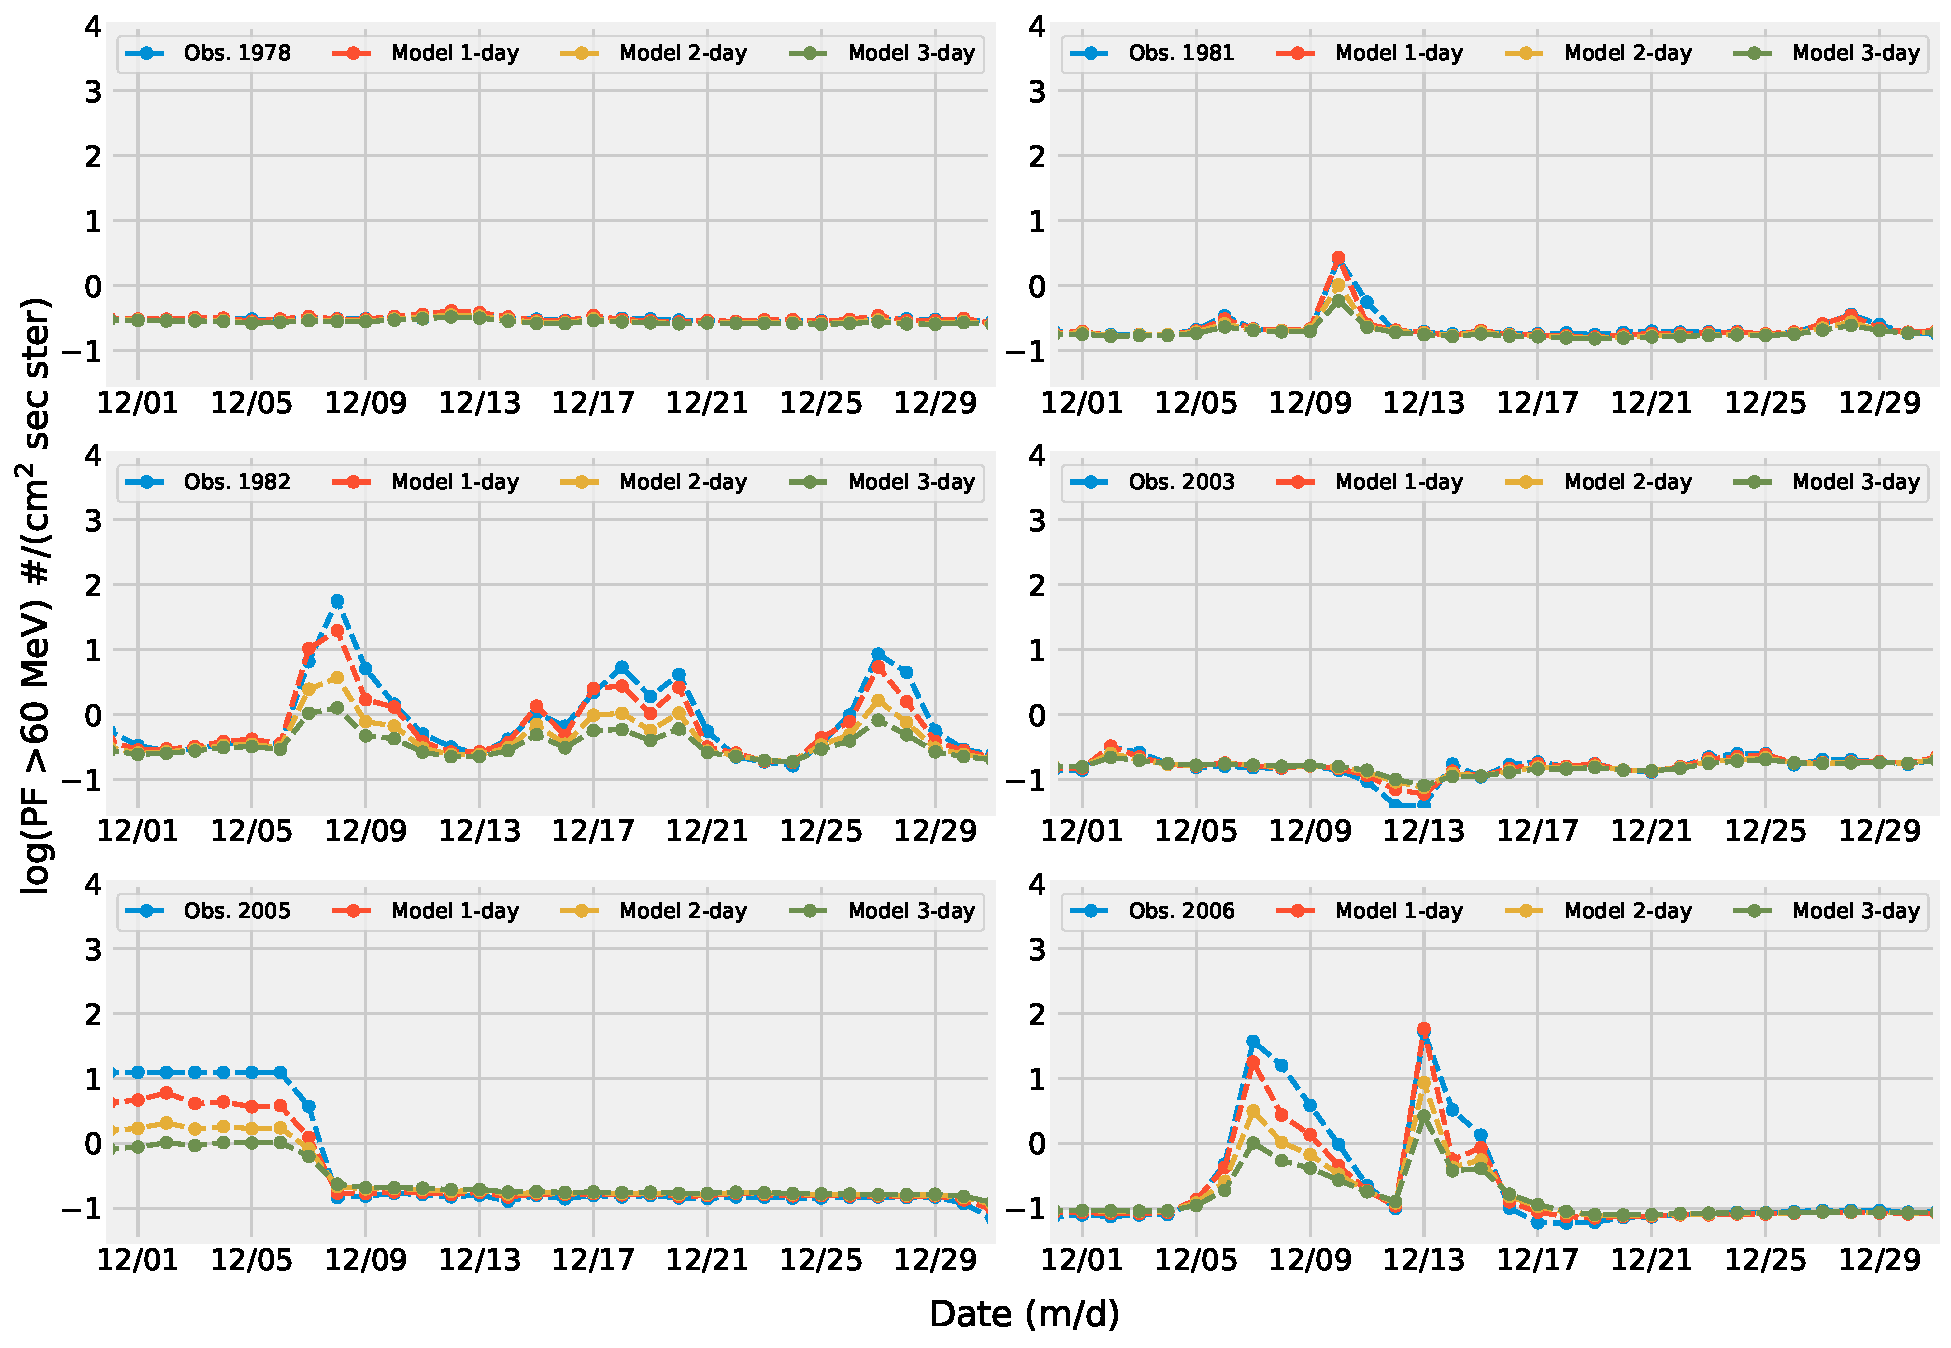
\includegraphics[width=\textwidth]{chapter4/figs/log_pf60/examples_60_tstset.pdf}}
    \caption{The model's forecasts for the out-of-sample testing set for the $>$60 MeV channel are shown at forecast horizons of 1 day, 2 days, and 3 days ahead, using samples of data from December in selected years mentioned in the top-left side of the plots.}
\label{fig_examples_pf60_tstset}
\end{figure}

From the visual inspection of the test set examples (Fig.~\ref{fig_examples_pf10_tstset}, ~\ref{fig_examples_pf30_tstset}, and~\ref{fig_examples_pf60_tstset}), we found that the predicted onset time, the peak time, and end times of SEP events were highly correlated with those of the observations, which implies that the model captured the temporal variations, as well as the trends in SEP flux.

\begin{table}[htp]
\centering
\caption{Summary of the performance results of the models for the validation and test sets.}
\begin{tabular}{lccccccccl}
\hline
\multicolumn{10}{c}{\textbf{Validation Set}}                                                                                                                 \\ \hline
       & \multicolumn{3}{c}{log PF \textgreater{}10 MeV} & \multicolumn{3}{c}{log PF \textgreater{}30 MeV} & \multicolumn{3}{c}{log PF \textgreater{}60 MeV} \\ \hline
Model Loss   & \multicolumn{3}{c}{0.0016}                      & \multicolumn{3}{c}{0.0010}                      & \multicolumn{3}{c}{0.0009}                      \\
Model Metric & \multicolumn{3}{c}{0.0329}                      & \multicolumn{3}{c}{0.0232}                      & \multicolumn{3}{c}{0.0218}                      \\ \hline
       & 1-Day          & 2-Day          & 3-Day         & 1-Day          & 2-Day          & 3-Day         & 1-Day    & 2-Day   & \multicolumn{1}{c}{3-Day}  \\ \hline
MAE    & 0.061          & 0.091          & 0.125         & 0.053          & 0.079          & 0.098         & 0.052    & 0.069   & 0.086                      \\
MSE    & 0.013          & 0.028          & 0.054         & 0.010          & 0.031          & 0.055         & 0.009    & 0.027   & 0.047                      \\
RMSE   & 0.114          & 0.168          & 0.233         & 0.098          & 0.176          & 0.234         & 0.097    & 0.164   & 0.217                      \\
MAPE   & 22.156         & 28.104         & 34.721        & 13.039         & 18.590         & 22.735        & 10.036   & 13.994  & 16.731                     \\ \hline
\multicolumn{10}{c}{\textbf{Test Set}}                                                                                                                       \\ \hline
       & \multicolumn{3}{c}{log PF \textgreater{}10 MeV} & \multicolumn{3}{c}{log PF \textgreater{}30 MeV} & \multicolumn{3}{c}{log PF \textgreater{}60 MeV} \\ \hline
Model Loss   & \multicolumn{3}{c}{0.0014}                      & \multicolumn{3}{c}{0.0011}                      & \multicolumn{3}{c}{0.0010}                      \\
Model Metric & \multicolumn{3}{c}{0.0333}                      & \multicolumn{3}{c}{0.0283}                      & \multicolumn{3}{c}{0.0250}                      \\ \hline
       & 1-Day          & 2-Day          & 3-Day         & 1-Day          & 2-Day          & 3-Day         & 1-Day    & 2-Day   & \multicolumn{1}{c}{3-Day}  \\ \hline
MAE    & 0.072          & 0.099          & 0.125         & 0.053          & 0.088          & 0.107         & 0.045    & 0.066   & 0.081                      \\
MSE    & 0.015          & 0.030          & 0.050         & 0.009          & 0.029          & 0.048         & 0.007    & 0.020   & 0.034                      \\
RMSE   & 0.121          & 0.172          & 0.224         & 0.094          & 0.170          & 0.218         & 0.082    & 0.141   & 0.184                      \\
MAPE   & 30.135         & 37.498         & 48.139        & 20.599         & 34.300         & 40.803        & 12.358   & 20.504  & 25.305                     \\ \hline
\end{tabular}
\label{table_performance}
\end{table}

To get further insight into the model's performance, we conducted an assessment of various skill scores, including True Positive (TP), True Negative (TN), False Positive (FP), and False Negative (FN). Additionally, skill score ratios such as Probability of Detection (POD), Probability of False Detection (POFD), False Alarm Rate (FAR), Critical Success Index (CSI), True Skill Statistic (TSS), and Heidke Skill Score (HSS). Detailed descriptions of these skill scores can be found in Appendix~\ref{skillscores_appendix}.
To extract individual SEP events from the test dataset, we implemented a threshold-based clustering algorithm. This algorithm uses the NOAA/SWPC warning threshold value of 10 pfu for the E $\geq$10 MeV channel. Upon analysis, we identified the number of detected SEP events for each output forecasting window and calculated the skill scores (Table~\ref{table_skillscores}). In the true test set, we identified 12 SEP events.

The evaluation of the model revealed notable trends as the length of the output forecasting window increased. The POD and CSI exhibited a declining pattern, indicating a reduced ability of the model to accurately detect and capture positive events (SEP occurrences) as the forecasting horizon extended further into the future. This suggests that the model's performance in identifying and capturing true positive instances diminishes with longer forecasting windows. Moreover, the POFD demonstrated an increasing trend, indicating an elevated rate of false positive predictions as the forecasting horizon lengthened. The model's propensity to generate false alarms rose with the lengthening forecasting window, leading to incorrect identification of non-events as positive events. Consequently, the TSS and HSS exhibited decreasing values, signifying a deterioration in the model's overall skill in accurately capturing and distinguishing between positive and negative instances. Overall, our skill scores are comparable with those reported by previous studies (Table~\ref{table_skillscores_comparison}). Although the UMASEP model does better than ours (i.e., has a higher POD), our FAR is much lower, thus, making fewer false alarms than the UMASEP model.

\begin{table}[htp]
\centering
\caption{Confusion matrix for the energy channel $\geq$10 MeV predictions in the test set.}
\label{table_skillscores}
\begin{tabular}{lccccccccccc}
\hline
E \textgreater{}10 MeV & No. events & TP & TN   & FP & FN \\ \hline
1-day ahead            & 15         & 21 & 1441 & 2  & 13 \\ \hline
2-day ahead            & 13         & 14 & 1441 & 2  & 20 \\ \hline
3-day ahead            & 5          & 5  & 1443 & 0  & 29 \\ \hline
\end{tabular}
\end{table}

\begin{table}[htp]
\centering
\caption{Comparing the skill scores with previous models. The dashed entries mean the data is unavailable (\citet{whitman_2022} for more details).}
\label{table_skillscores_comparison}
\resizebox{\textwidth}{!}{%
\begin{tabular}{lccccccccc}
\hline
\multicolumn{1}{c}{\textbf{Model}}       &            & \textbf{POD} & \textbf{FAR} & \textbf{TSS} & \textbf{HSS} & \textbf{POFD} & \textbf{CSI} & \multicolumn{1}{l}{\textbf{Accuracy}} & \multicolumn{1}{l}{\textbf{Precision}} \\ \hline
\multirow{3}{*}{Our BiLSTM model}        & 1-Day      & 0.618        & 0.087        & 0.531        & 0.732        & 0.001         & 0.583        & 0.99                                  & 0.913                                  \\ \cline{2-10} 
                                         & 2-Day      & 0.412        & 0.125        & 0.287        & 0.553        & 0.001         & 0.389        & 0.985                                 & 0.875                                  \\ \cline{2-10} 
                                         & 3-Day      & 0.147        & 0            & 0.147        & 0.252        & 0             & 0.147        & 0.980                                 & 1                                      \\ \hline
\multicolumn{2}{l}{UMASEP-10 \citep{Nunez_2011}}           & 0.822        & 0.219        & ---          & ---          & ---           & ---          & ---                                   & ---                                    \\ \hline
\multicolumn{2}{l}{PCA \citep{Papaioannou_2018}}     & 0.587        & 0.245        & ---          & 0.65         & ---           & ---          & ---                                   & ---                                    \\ \hline
\multicolumn{2}{l}{SPARX \citep{Dalla_2017}}         & 0.5          & 0.57         & ---          & ---          & 0.32          & 0.3          & ---                                   & ---                                    \\ \hline
\multicolumn{2}{l}{SPRINTS \citep{engell_2017}}      & 0.56         & 0.34         & ---          & 0.58         & ---           & ---          & ---                                   & ---                                    \\ \hline
\multicolumn{2}{l}{REleASE \citep{malandraki_2018}} & 0.63         & 0.3          & ---          & ---          & ---           & ---          & ---                                   & ---                                    \\ \hline
\end{tabular}
}
\end{table}

\section{Conclusions}
\label{sec_ch4_conclusion}
Forecasting the SEP flux is a crucial task in heliophysics since it affects satellite operations, astronaut safety, and ground-based communication systems. It is a challenging task due to its non-linear, non-stationary, and complex nature. Machine learning techniques, particularly neural networks, have shown promising results in predicting SEP flux.
In this study, we developed and trained BiLSTM neural network models to predict the daily-averaged integral flux of SEP at 1-day, 2-day, and 3-day ahead, for the energy channels $>$10 MeV, $>$30 MeV, and $>$60 MeV.
We used a combination of solar and interplanetary magnetic field indices from the OMNIWeb database for the past 4 solar cycles as input to the model.
We compared the models with baseline models and evaluated them using the Huber loss and the error metrics in Appendix~\ref{eval_appendix}.

The data windowing method we used, based on the MIMO strategy, eliminates the need to feed the output forecast as input back into the model and that allows to do forecasting relatively far into the future while maintaining decent results (e.g., the MSE is ranging between 0.007 and 0.015 for 1-day forecasting in the test set, compared to an MSE of 0.236 for a persistence model. See Table~\ref{table_performance}).
The results show that the model can make reasonably accurate predictions given the difficulty and complexity of the problem.
The MSE was ranged between 0.009 and 0.055 for the validation set, and between 0.007 and 0.05 for the test set.
The correlations between the observations and predictions were $>$0.9 for the validation and test sets (Fig.~\ref{fig_model_vs_obs_valset} and Fig.~\ref{fig_model_vs_obs_tstset}).
Nevertheless, the mean temporal correlation was $\sim$0.8 for the test set (Fig.~\ref{fig_crosscorr_tstset}).
Although our models performed well, we observed a relatively large discrepancy between the predictions and the observations in the $>$30 MeV energy band.

The findings of this study underscore the challenges encountered by the forecasting model in accurately predicting SEP data over longer time periods. As the length of the output forecasting window increased, the model's ability to detect true positives and its overall skill in differentiating positive and negative instances diminished. Additionally, the model displayed an elevated rate of false negative predictions, indicating an increased tendency to generate misses as the forecasting horizon extended. These results highlight the importance of carefully considering the appropriate forecasting window length for SEP data to ensure the model's optimal performance. Our skill scores generally align with those from previous works (Table~\ref{table_skillscores_comparison}). There are variations in the metrics' values across different studies, highlighting the complexities and nuances associated with each study. Nevertheless, it is important to acknowledge that the statistical significance of the results in this study is limited due to data averaging. Future studies should consider incorporating hourly data, as this is likely to result in a greater number of identified events.
The model can provide short-term predictions, which can be used to anticipate the behavior of the near-Earth space environment. These predictions have important implications for space weather forecasting, which is essential for protecting satellites, spacecraft, and astronauts from the adverse effects of solar storms.

Multiple techniques exist for identifying the optimal combination of hidden layers and neurons for a given task such as empirical methods, parametric methods, and the grid search cross-validation method, which we will explore in future work.
The observed reduction in correlation necessitates further investigation to determine its origin, whether stemming from tangible causal factors or potential aberrations within the model or data.
We plan to expand upon this work by performing short-term forecasting using hourly-averaged data. This extension will involve integrating additional relevant features such as the location and area of active regions and coronal holes on the Sun.

BiLSTM networks are particularly useful for tasks involving sequential data such as timeseries forecasting. Given their capacity to handle input sequences in both directions in time and capture long-term dependencies, they are valuable in a broad range of applications. Nonetheless, one should carefully consider their data requirements and computational complexity before adopting them.
Our results emphasize that the use of deep learning models in forecasting tasks in heliophysics are promising and encouraging, as pointed out by \citet{zhang_2022}.

This work is a stepping stone towards real-time forecasting of SEP flux based on the public-available datasets. As an extension, we are currently working on developing a set of models that deliver near-real time prediction of SEP fluxes at multiple energy bands, multiple forecasting windows, with hourly-averaged data resolution, with a more sophisticated model architecture, as well as more features that address the state of solar activity more comprehensively. 
We plan to extend the analysis to include more recent data from solar cycle 25, in order to improve the accuracy of the models.
In conclusion, our study highlights the potential of using BiLSTM neural networks for forecasting SEP integral fluxes. Our models provide a promising approach for predicting the near-Earth space environment too, which is crucial for space weather forecasting and ensuring the safety of our space assets. Our findings contribute to the growing body of literature on the applications of deep learning techniques in heliophysics and space weather forecasting.

	\chapter{Summary}
\label{chapter5}
In this final chapter, I present a comprehensive summary of the key findings from the dissertation's chapters, providing insights into the analysis of EUV waves, solar type III bursts, and SEP modeling and forecasting. The exploration of CBFs and the introduction of the Wavetrack tool have significantly contributed to our nuanced understanding of solar dynamics. As we look towards the future, the extension of the CBF dataset promises deeper insights into their kinematics, while the utilization of multi-wavelength observations from LOFAR, PSP, and Solar Orbiter aims to unravel the origin and evolution of energetic particles in the solar corona. Furthermore, the development of interpretable deep learning models, driven by higher resolution data, holds the key to advancing SEP forecasting capabilities. These future endeavors underscore the commitment to refining models, incorporating advanced data analysis techniques, and leveraging cutting-edge observational tools to unlock new dimensions in our comprehension of space weather phenomena.

Chapter~\ref{chapter2} centered on the analysis of base-difference images obtained from the SDO/AIA instrument to investigate EUV waves. Key kinematic parameters, including shock speed, acceleration, intensity, and thickness, were computed. SOHO/LASCO measurements up to 17\rsun were incorporated to enhance the understanding of shock plasma parameters. Kinematic measurements played a pivotal role in generating 3D geometric models of wavefronts and informing plasma diagnostics using MHD and DEM models. The use of shock kinematic measurements facilitated the fitting of geometric spheroid surface models. Parametrized relationships between plasma parameters were explored to uncover connections and interdependencies. The study also introduced Wavetrack, an automated tool for identifying and monitoring dynamic coronal phenomena. Its application to CBF events revealed proficiency in tracking complete pixel maps, aiding in understanding CBF evolution. Limitations were acknowledged, and future work will address them for enhanced versatility. The methodology holds promise for extensive application in solar dynamic features and observational datasets.

Chapter~\ref{chapter3} delved into the analysis of type III bursts during the second near-Sun encounter period of PSP. Sixteen separate radio bursts were observed using the PSP/FIELDS instrument and LOFAR ground-based telescope. A semi-automated pipeline facilitated data analysis, alignment, and interferometric imaging. Uniform frequency drifts among bursts suggested related origins. Interferometric observations located type III emissions off the southeast limb of the Sun, hinting at a single source of electron beams low in the corona. Magnetic extrapolation favored the active region AR12737 as the source, aligning with previous studies. However, caution was advised regarding potential deviations in magnetic field configurations near active regions. The study also explored discrepancies in observed and modeled density profiles, attributing them to scattering and propagation effects. Future work will integrate TDoA technique and Solar Orbiter observations for a more comprehensive analysis of solar radio bursts.

The pioneering multi-event exploration in Chapter~\ref{chapter4} focused on Sun-to-Earth SEP simulations, investigating 62 eruptive events with EUV CBFs. The SPREAdFAST framework was employed to analyze coronal diffusive shock acceleration and interplanetary propagation. Input spectra for coronal proton acceleration were derived from quiet-time suprathermal spectra, exhibiting influences of solar corona conditions on proton acceleration. Comparison with in situ observations demonstrated overall alignment, validating the efficiency of the SPREAdFAST model. Discrepancies at the highest energies were noted, prompting future work to refine modeling and incorporate three-dimensional transport effects. The study also introduced a BiLSTM neural network model for forecasting SEP integral flux at 1 AU, showcasing promising results for short-term predictions with implications for space weather forecasting.

In conclusion, the dissertation contributions include a nuanced understanding of EUV waves, an automated tool for tracking coronal phenomena, insights into type III bursts and their sources, and advancements in SEP simulations and forecasting using deep learning. Future directions involve addressing limitations, refining models, and incorporating more recent data for a comprehensive understanding of solar dynamics and space weather forecasting.

\section{Future Work}
The quest to understand the Sun's ever-changing nature continues. Future research in heliophysics holds immense potential to expand our knowledge and improve space weather forecasting.

One crucial area lies in expanding the data pool for EUV waves. By studying EUV waves observed throughout various solar cycle phases, we can investigate how the Sun's cyclical activity influences their behavior. Similarly, incorporating a broader range of active regions with diverse magnetic configurations into the analysis of solar radio bursts will be key. This will provide a more comprehensive picture of their characteristics across different solar activity levels.

The next leap forward hinges on leveraging multi-wavelength observations. Instruments like LOFAR, Parker Solar Probe, and Solar Orbiter, each providing data at different wavelengths, will be instrumental. By combining these views, we can gain a deeper understanding of how energetic particles and radio bursts originate and evolve within the solar corona. Additionally, incorporating high-resolution data will allow for a more detailed and accurate representation of the dynamic processes at play.

Furthermore, future studies should account for the impact of scattering and propagation phenomena on both SEPs and radio burst observations. Refining models to account for these effects will significantly enhance their accuracy for forecasting purposes.

Beyond data granularity, expanding the features used in SEP prediction models is crucial.  Including characteristics of active regions, for example, could provide a more nuanced forecasting capability.  Additionally, the implementation of advanced interpretable deep learning architectures holds promise for enhancing model reliability and reducing forecasting errors.

The ultimate goal lies in developing real-time analysis tools for space weather forecasting. These tools will integrate data from newly commissioned instruments and spacecraft, coupled with the incorporation of advanced methodologies. By refining our understanding of solar dynamics and improving the accuracy of predictive models, we can ultimately provide early warnings and more accurate risk assessments for space weather events.

%Future work will expand our understanding of CBFs by extending the list of observed events, aiming for a more comprehensive analysis of their kinematics and early-stage evolution within the complex coronal environment. Leveraging multi-wavelength remote-sensing observations from LOFAR and Solar Orbiter will be instrumental in probing the origin and evolution of energetic particles in the solar corona. The integration of high-resolution data from these sources will provide a more detailed and accurate representation of the dynamic processes involved. Additionally, future research endeavors will focus on developing interpretable deep learning models for SEP forecasting. These models, built with higher resolution data, aim to enhance the precision and reliability of predictions, contributing to the advancement of space weather forecasting capabilities. The incorporation of advanced methodologies and diverse observational datasets is essential for refining our comprehension of solar dynamics and improving the accuracy of predictive models.




%Expanding the sample size of CBF events studied could provide a more comprehensive view and validate the statistical relationships derived in this thesis. Future work should aim to include CBFs from different phases of the solar cycle to factor in the cycle's influence on these phenomena.
%
%For solar radio bursts, including a broader spectrum of active regions with varied magnetic configurations would be beneficial. Observations across different levels of solar activity could deliver additional context to our current understanding. Leveraging multi-wavelength remote-sensing observations from LOFAR, Parker Solar Probe, and Solar Orbiter would be instrumental in probing the origin and evolution of energetic particles in the solar corona. The integration of high-resolution data from these sources will provide a more detailed and accurate representation of the dynamic processes involved.
%Investigations should also examine the effects of scattering and propagation processes on SEP and radio burst observations for more refined modeling approaches.
%
%To tackle the limitations around data granularity for SEP forecasting, future studies should aim to incorporate high-resolution data. Hourly-averaged or even higher resolution datasets may unveil more intricate patterns and abrupt changes in SEP events, improving forecasting accuracy. Extending the features used for SEP prediction models to encompass other diagnostic parameters, such as the characteristics of active regions, could provide a more nuanced forecasting capability.
%The implementation of advanced interpretable deep learning architectures could be pursued to enhance model reliability and reduce the likelihood of forecasting errors.
%
%Development of real-time analysis tools for space weather forecasting that assimilate data from newly commissioned instruments and spacecraft, as well as the incorporation of advanced methodologies, is essential for refining our comprehension of solar dynamics and improving the accuracy of predictive models and will provide early warning capabilities and more accurate risk assessments.

%The research presented in this thesis establishes an important foundation and provides a precursor for future advances that can build upon the present work. Some open questions and promising areas for future investigations include:
%
%- Additional coronal wave statistical studies using expanded event samples and new imaging datasets from Solar Orbiter and ground observatories to improve generalizability of findings.
%
%- Incorporating 3D analytical and numerical coronal wave propagation models for more physics-based forecasting approaches. 
%
%- Modeling mechanisms for type III radio burst onset and time profiles using particle-in-cell and MHD models. 
%
%- Ensemble forecasting models for SEP events combining multiple machine learning algorithms trained on multi-mission data.
%
%- Leveraging new solar observatory missions and assimilative models within operational prediction systems for real-time space weather forecasts.
%
%- Exploring applications of deep learning and physics-informed machine learning to additional outstanding problems in heliophysics and astrophysics.
%
%In summary, the present work opens exciting avenues for more cross-disciplinary studies synthesizing heliophysics domain knowledge with cutting-edge data science and artificial intelligence methods. The new generation of solar, heliospheric and geospace missions will yield transformative observations to continue advancing both science understanding and predictive capabilities.
	
	\huge
\textbf{Publications}
\vspace{1.5cm}

\Large
\textbf{First-Author Papers}
\vspace{0.1cm}

\normalsize
\begin{enumerate}
	\item \textbf{Nedal, M.}, Kozarev, K., Miteva, R., Stepanyuk, O., Dechev, M., "Characterization of the Early Dynamics of Solar Coronal Bright Fronts", Bulgarian Astronomical Journal, ..., 2024. \textit{under review}.
	
	\item \textbf{Nedal, M.}, Kozarev, K., Zhang, P., and Zucca, P., "Coronal diagnostics of solar type III radio bursts using LOFAR and PSP observations", Astronomy and Astrophysics vol. 680, 2023. doi: 10.1051/0004-6361/202347041.
	
	\item \textbf{Nedal, M.}, Kozarev, K., Arsenov, N., and Zhang, P., "Forecasting solar energetic proton integral fluxes with bi-directional long short-term memory neural networks", Journal of Space Weather and Space Climate, vol. 13, 2023. doi: 10.1051/swsc/2023026.
\end{enumerate}

\vspace*{0.15cm}

\Large
\textbf{Co-Author Papers}
\vspace{0.1cm}

\normalsize
\begin{enumerate}
	\item Kozarev, K., \textbf{Nedal, M.}, Miteva, R., Dechev, M., and Zucca, P., "A Multi-Event Study of Early-Stage SEP Acceleration by CME-Driven Shocks—Sun to 1 AU", Frontiers in Astronomy and Space Sciences, vol. 9, 2022. doi: 10.3389/fspas.2022.801429.
	
	\item Stepanyuk, O., Kozarev, K., and \textbf{Nedal, M.}, "Multi-scale image preprocessing and feature tracking for remote CME characterization", Journal of Space Weather and Space Climate, vol. 12, 2022. doi: 10.1051/swsc/2022020.
	
	\item Miteva, R., \textbf{Nedal, M.}, Samwel, S. W., and Temmer, M., "Parameter Study of Geomagnetic Storms and Associated Phenomena: CME Speed De-Projection vs. In Situ Data", Universe, vol. 9, no. 4, 2023. doi: 10.3390/universe9040179.
	
	\item Whitman, K., ..., \textbf{Nedal, M.}, “Review of Solar Energetic Particle Prediction Models", Advances in Space Research, vol. 72, no. 12, pp. 5161–5242, 2023. doi: 10.1016/j.asr.2022.08.006.
	
	\item Abuelezz, O., Mahrous, A., Cilliers, P., Fleury, R., Youssef, M., \textbf{Nedal, M.}, Yassen, A., "Neural network prediction of the topside electron content over the Euro-African sector derived from Swarm-A measurements", Advances in Space Research, vol. 67, no. 4, pp. 1191–1209, 2021. doi: 10.1016/j.asr.2020.11.009.
\end{enumerate}
	\huge
\textbf{Requirements}
\vspace{1.5cm}

\large
PhD requirements according to the Bulgarian Academy of Sciences.

\normalsize

\begin{table}[!htp]
\centering
\LARGE
\resizebox{\textwidth}{!}{%
	\begin{tabular}{lcc}
		\hline
		\textbf{Execution of educational program}                                                                                                                   & \multicolumn{1}{l}{\textbf{Required minimum}} & \multicolumn{1}{l}{\textbf{PhD student points}} \\ \hline
		I. Exam taken on basic specialized topic (1$\times$40 pts required)                                                                                                & 40                                            & 40                                              \\ \hline
		II. Additional specialized courses (2$\times$20 required)                                                                                                          & 40                                            & 60                                              \\ \hline
		III. Exam taken on foreign language proficiency (1$\times$25 pts unless waived)                                                                                    & 25                                            & 25                                              \\ \hline
		IV. Exam taken on computer skills (1$\times$25 pts)                                                                                                                & 25                                            & 25                                              \\ \hline
		\textbf{Required minimum points/total points I.-IV.}                                                                                                      & \textbf{130}                                  & \textbf{150}                                    \\ \hline
		\textbf{Execution of educational program}                                                                                                                   & \textbf{Required minimum}                     & \textbf{PhD student points}                     \\ \hline
		V. Presentation at a scientific forum abroad (32 pts)\\or a scientific forum in Bulgaria (24 pts)                                                            & 40                                            & 408                                             \\ \hline
		\textbf{Required minimum points/total points V.}                                                                                                          & \textbf{40}                                   & \textbf{408}                                    \\ \hline
		\textbf{Publication of scientific work on the dissertation topic}                                                                                           & \textbf{Required minimum}                     & \textbf{PhD student points}                     \\ \hline
		VI. Publication in an international scientific journal,\\ international proceedings journal, or a Bulgarian scientific journal\\with international recognition & 30                                            & 110                                             \\ \hline
		\textbf{Required minimum points / total points VI.}                                                                                                         & \textbf{30}                                   & \textbf{110}                                    \\ \hline
		\textbf{Required minimum total points}                                                                                                                      & \textbf{200}                                  & \textbf{668 (334\%)}                             \\ \hline
	\end{tabular}%
}
\end{table}
	
	\bibliographystyle{aa}
	\bibliography{refs}
	
\end{document}